\chapter{Thực nghiệm và thảo luận}
\label{ch:thuc-nghiem}

Chương này trình bày toàn bộ kết quả thực nghiệm và các phân tích nhằm trả lời 5 câu hỏi nghiên cứu (RQ1--RQ5) đã đặt ra. Các thực nghiệm được tổ chức theo hai hướng nghiên cứu chính:
(1) \textit{Hướng thứ nhất -- Khảo sát phân loại đa mức PHQ-9:} Đánh giá đóng góp của các nhóm đặc trưng ($F_1 \to F_4$), tinh chỉnh siêu tham số và đối chuẩn thuật toán, khảo sát biến thiên hiệu năng theo độ chi tiết nhãn ($T_2 \to T_5$), phân tích tương quan sinh lý và hình chiếu PCA, cùng thử nghiệm mở rộng dữ liệu đa chu kỳ NHANES ($N = 14.581$).
(2) \textit{Hướng thứ hai -- Khảo sát phân loại phân cấp và thứ bậc trên $T_3$:} Đánh giá có hệ thống 8 cấu hình mô hình thực nghiệm ($E_0 \to E_7$) trên không gian 3 nhóm ($C_0, C_1, C_2^+$); phân tích sự đánh đổi sai số theo ma trận chi phí Bayes; kiểm định ngoại suy theo dòng thời gian trên chu kỳ độc lập NHANES 2015--2016; và thảo luận tổng hợp 4 mô hình tiêu biểu đại diện cho các mục tiêu thực tế khác nhau.

\section{Thiết lập thực nghiệm và môi trường tính toán}
\label{sec:moi-truong-thuc-nghiem}

Môi trường thực nghiệm được thiết lập thống nhất:
\begin{itemize}
    \item \textbf{Phần cứng:} Máy trạm Apple Silicon (ARM64, M-series), bộ nhớ 16 GB RAM, ổ cứng SSD.
    \item \textbf{Môi trường phần mềm:} macOS Darwin Kernel 24.6.0; Python 3.13 chạy trong môi trường ảo hóa độc lập (\texttt{.venv}).
    \item \textbf{Thư viện tính toán:} \texttt{scikit-learn} 1.9.1 (các thuật toán học máy, tiền xử lý và kiểm định chéo); \texttt{xgboost} 3.4.1; \texttt{scipy} 1.18.1 (tối ưu hóa phi tuyến L-BFGS-B cho mô hình OLR); \texttt{numpy} 2.5.3 và \texttt{pandas} 3.0.6; \texttt{matplotlib} 3.11.2 (trực quan hóa dữ liệu và xuất biểu đồ 300 DPI).
    \item \textbf{Kiểm soát ngẫu nhiên:} Hạt giống \texttt{random\_state = 42} được cố định trên tất cả các phép chia fold, khởi tạo mô hình và lấy mẫu bootstrap nhằm bảo đảm tính tái lập kết quả.
\end{itemize}

\section{Đánh giá đóng góp của các nhóm đặc trưng (Feature Ablation)}
\label{sec:feature-ablation}

\subsection{Thiết lập thực nghiệm}
Thực nghiệm Feature Ablation nhằm trả lời câu hỏi nghiên cứu \textbf{RQ1}: Khảo sát mức độ đóng góp của bốn nhóm đặc trưng lũy tiến ($F_1 \to F_4$) đối với bài toán 5 mức độ $T_5$ ($C_0 \to C_4$). Thực nghiệm được thực hiện thông qua Stratified 5-Fold Cross-Validation trên tập phát triển Legacy ($N = 4.045$). Bốn thuật toán học máy cơ sở được đánh giá song song gồm: Logistic Regression (LR), Decision Tree (DT), Random Forest (RF) và XGBoost.

\subsection{Kết quả thực nghiệm}
Kết quả out-of-fold chi tiết được tổng hợp trong Bảng \ref{tab:ablation-results}. Hình \ref{fig:ablation-comparison} thể hiện xu hướng biến thiên của Macro-F1 trên các không gian đặc trưng.

\begin{table}{Kết quả thực nghiệm Feature Ablation trên tập Legacy Development ($N = 4.045$, 5 lớp $T_5$)}
\centering
\footnotesize
\setlength{\tabcolsep}{3pt}
\label{tab:ablation-results}
\begin{tabularx}{\textwidth}{l c l >{\centering\arraybackslash}X >{\centering\arraybackslash}X >{\centering\arraybackslash}X}
\toprule
\textbf{Nhóm} & \textbf{$d$} & \textbf{Mô hình ML} & \textbf{Macro-F1 (Mean $\pm$ SD)} & \textbf{Balanced Acc (Mean $\pm$ SD)} & \textbf{Weighted-F1 (Mean $\pm$ SD)} \\
\midrule
\multirow{4}{*}{\textbf{$F_1$}} & \multirow{4}{*}{10} 
  & Logistic Regression & 0.1900 $\pm$ 0.0164 & 0.2420 $\pm$ 0.0299 & 0.4926 $\pm$ 0.0209 \\
& & Decision Tree        & 0.2081 $\pm$ 0.0121 & 0.2090 $\pm$ 0.0133 & 0.5926 $\pm$ 0.0081 \\
& & Random Forest       & 0.2052 $\pm$ 0.0072 & 0.2090 $\pm$ 0.0065 & 0.6314 $\pm$ 0.0107 \\
& & XGBoost             & 0.2173 $\pm$ 0.0147 & 0.2295 $\pm$ 0.0220 & 0.5577 $\pm$ 0.0072 \\
\midrule
\multirow{4}{*}{\textbf{$F_2$}} & \multirow{4}{*}{19} 
  & Logistic Regression & 0.2338 $\pm$ 0.0041 & 0.2942 $\pm$ 0.0299 & 0.5648 $\pm$ 0.0092 \\
& & Decision Tree        & 0.2319 $\pm$ 0.0154 & 0.2357 $\pm$ 0.0185 & 0.6144 $\pm$ 0.0093 \\
& & Random Forest       & 0.2350 $\pm$ 0.0180 & 0.2353 $\pm$ 0.0155 & 0.6557 $\pm$ 0.0097 \\
& & XGBoost             & 0.2447 $\pm$ 0.0143 & 0.2594 $\pm$ 0.0187 & 0.6002 $\pm$ 0.0123 \\
\midrule
\multirow{4}{*}{\textbf{$F_3$}} & \multirow{4}{*}{29} 
  & Logistic Regression & 0.2390 $\pm$ 0.0084 & 0.3194 $\pm$ 0.0284 & 0.5637 $\pm$ 0.0071 \\
& & Decision Tree        & 0.2388 $\pm$ 0.0127 & 0.2408 $\pm$ 0.0148 & 0.6195 $\pm$ 0.0100 \\
& & Random Forest       & 0.2299 $\pm$ 0.0045 & 0.2314 $\pm$ 0.0047 & 0.6671 $\pm$ 0.0085 \\
& & XGBoost             & 0.2588 $\pm$ 0.0402 & 0.2713 $\pm$ 0.0490 & 0.6224 $\pm$ 0.0154 \\
\midrule
\multirow{4}{*}{\textbf{$F_4$}} & \multirow{4}{*}{34} 
  & Logistic Regression & 0.2399 $\pm$ 0.0148 & \textbf{0.3216 $\pm$ 0.0508} & 0.5591 $\pm$ 0.0112 \\
& & Decision Tree        & 0.2412 $\pm$ 0.0175 & 0.2450 $\pm$ 0.0206 & 0.6181 $\pm$ 0.0098 \\
& & Random Forest       & 0.2232 $\pm$ 0.0099 & 0.2253 $\pm$ 0.0075 & \textbf{0.6625 $\pm$ 0.0091} \\
& & XGBoost             & \textbf{0.2707 $\pm$ 0.0428} & 0.2837 $\pm$ 0.0485 & 0.6344 $\pm$ 0.0148 \\
\bottomrule
\end{tabularx}
\end{table}


\begin{figure}[htbp]{So sánh hiệu năng Macro-F1 của 4 thuật toán trên các nhóm đặc trưng lũy tiến $F_1 \to F_4$}
\centering
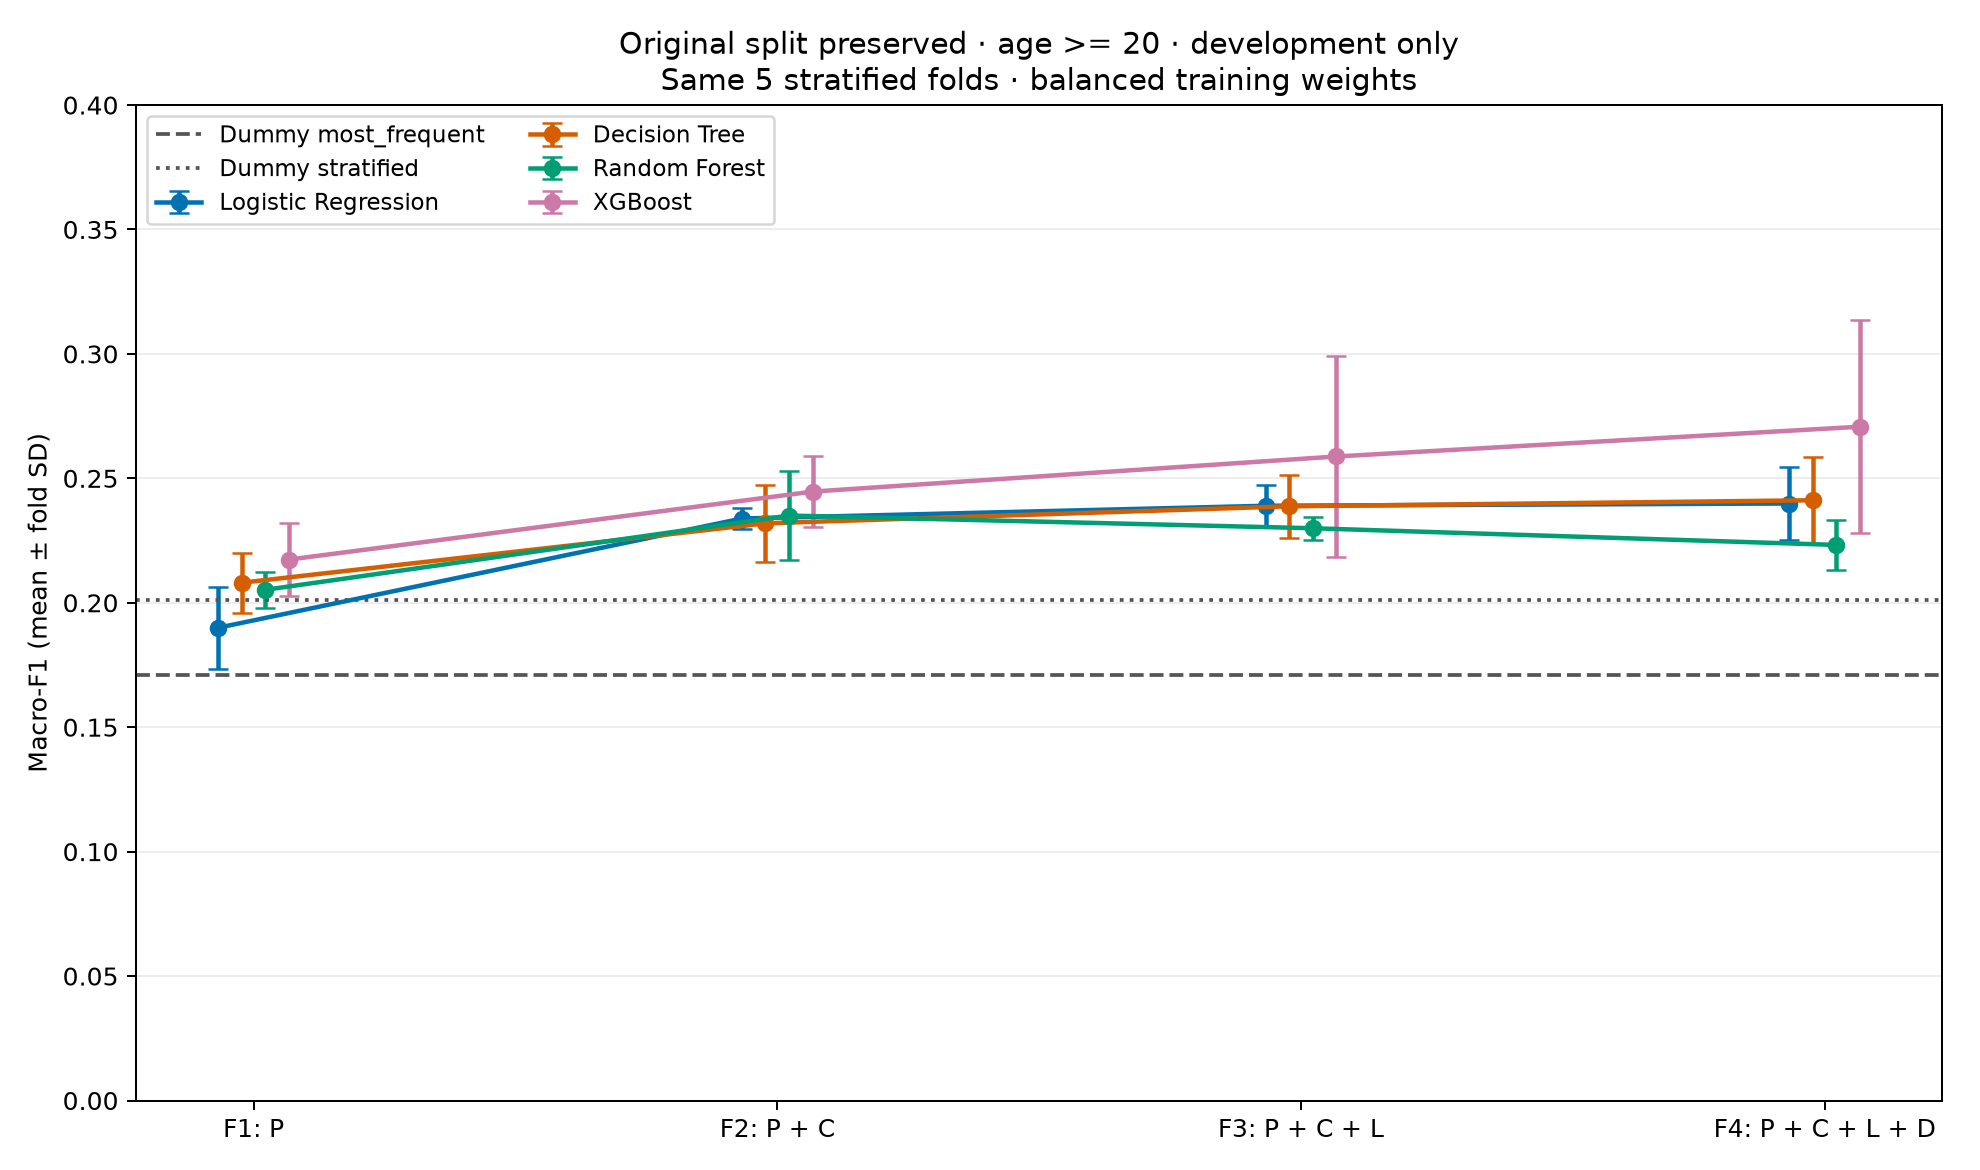
\includegraphics[width=0.9\textwidth]{figures/feature_group_comparison_final_protocol.png}
\label{fig:ablation-comparison}
\end{figure}
\FloatBarrier

\subsection{Phân tích kết quả}
Từ kết quả Bảng \ref{tab:ablation-results}, một số phát hiện được ghi nhận:
\begin{enumerate}
    \item \textbf{Đóng góp của nhóm Tiền sử bệnh lý ($F_1 \to F_2$):} Nhóm $F_1$ (10 biến gồm thể chất, huyết áp và 5 xét nghiệm máu) chỉ mang lại Macro-F1 khiêm tốn (0.1900 với LR và 0.2173 với XGBoost). Khi bổ sung 9 biến tiền sử bệnh mạn tính ở nhóm $F_2$, hiệu năng tăng rõ rệt trên tất cả các mô hình: LR tăng từ 0.1900 lên 0.2338 (+23.1\%), RF tăng từ 0.2052 lên 0.2350 (+14.5\%), và XGBoost tăng từ 0.2173 lên 0.2447 (+12.6\%). Điều này cho thấy tiền sử bệnh mạn tính cung cấp thông tin hữu ích cho việc phân tầng nguy cơ.
    \item \textbf{Đóng góp của nhóm Lối sống và Nhân khẩu học ($F_3, F_4$):} Nhóm thói quen sinh hoạt (giấc ngủ, vận động thể lực, hút thuốc, rượu bia) và nhân khẩu học (tuổi, giới tính, học vấn, tỷ lệ thu nhập) tiếp tục nâng hiệu năng của XGBoost lên mức Macro-F1 cao nhất là \textbf{0.2707 $\pm$ 0.0428} (Balanced Accuracy = 0.2837 $\pm$ 0.0485).
    \item \textbf{Sự khác biệt giữa Weighted-F1 và Macro-F1:} Weighted-F1 luôn đạt mức cao (0.49 -- 0.67) do bị chi phối bởi lớp đa số $C_0$ (chiếm ~75\%). Ngược lại, Macro-F1 dao động quanh mức 0.19 -- 0.27, phản ánh đúng mức độ khó khăn khi nhận diện các lớp có triệu chứng.
\end{enumerate}

\section{Tinh chỉnh siêu tham số và khảo sát mô hình kết hợp}
\label{sec:tuning-va-ensemble}

\subsection{Tinh chỉnh Nested Cross-Validation và Đối chuẩn thuật toán}
Để lựa chọn cấu hình mô hình cơ sở một cách khách quan và hạn chế thiên lệch lạc quan, nghiên cứu áp dụng quy trình kiểm định chéo lồng nhau (Nested CV): Outer 5 folds đánh giá khả năng khái quát hóa, Inner 3 folds thực hiện \texttt{RandomizedSearchCV} với 12 cấu hình siêu tham số trên độ đo Macro-F1.

Kết quả đối chuẩn giữa các thuật toán học máy cơ sở qua Outer Nested CV được tổng hợp trong Bảng \ref{tab:nested-cv-comparison}.

\begin{table}{Kết quả đánh giá đối chuẩn các thuật toán học máy cơ sở qua Nested Cross-Validation (5 lớp $T_5$)}
\centering
\footnotesize
\setlength{\tabcolsep}{3.5pt}
\label{tab:nested-cv-comparison}
\begin{tabularx}{\textwidth}{p{3.2cm} c >{\centering\arraybackslash}X >{\centering\arraybackslash}X >{\centering\arraybackslash}X c}
\toprule
\textbf{Thuật toán ML} & \textbf{Đặc trưng} & \textbf{Macro-F1 (Mean $\pm$ SD)} & \textbf{Balanced Acc (Mean $\pm$ SD)} & \textbf{Weighted-F1 (Mean $\pm$ SD)} & \textbf{$\Delta$ so với Baseline} \\
\midrule
Logistic Regression & $F_4$ (34) & 0.2407 $\pm$ 0.0173 & \textbf{0.3253 $\pm$ 0.0532} & 0.5599 $\pm$ 0.0128 & $+0.0009$ \\
Decision Tree (Gini) & $F_4$ (34) & 0.2412 $\pm$ 0.0175 & 0.2450 $\pm$ 0.0206 & 0.6181 $\pm$ 0.0098 & $0.0000$ \\
XGBoost (Tuned) & $F_3$ (29) & 0.2516 $\pm$ 0.0267 & 0.2658 $\pm$ 0.0355 & 0.6130 $\pm$ 0.0152 & $-0.0071$ \\
XGBoost (Tuned) & $F_4$ (34) & 0.2621 $\pm$ 0.0353 & 0.2743 $\pm$ 0.0373 & 0.6196 $\pm$ 0.0195 & $-0.0087$ \\
\textbf{Random Forest (Frozen)} & $F_4$ (34) & \textbf{0.2755 $\pm$ 0.0270} & 0.2983 $\pm$ 0.0325 & \textbf{0.6437 $\pm$ 0.0087} & \textbf{+0.0523} \\
\bottomrule
\end{tabularx}
\end{table}



\textbf{Phân tích kết quả và lý do lựa chọn Random Forest làm mô hình cơ sở chính:}
Từ Bảng \ref{tab:nested-cv-comparison}, Random Forest đạt chỉ số Macro-F1 trung bình cao nhất trong nhóm các mô hình phẳng được khảo sát là \textbf{0.2755 $\pm$ 0.0270} và Weighted-F1 đạt \textbf{0.6437 $\pm$ 0.0087}, cải thiện \textbf{+0.0523} so với cấu hình mặc định chưa tinh chỉnh ($0.2232$).

Lý do lựa chọn Random Forest được xác định dựa trên kết quả thực nghiệm:
\begin{enumerate}
    \item \textit{Đánh giá khách quan trên các chỉ số:} Logistic Regression đạt Balanced Accuracy cao hơn ($0.3253 \pm 0.0532$) nhờ mặt phẳng phân tách tuyến tính trơn mượt phân bổ dự đoán sang các lớp nhỏ, nhưng Macro-F1 lại thấp hơn ($0.2407$). XGBoost đạt Macro-F1 là $0.2621 \pm 0.0353$ nhưng có độ lệch chuẩn lớn hơn giữa các fold so với Random Forest.
    \item \textit{Tính ổn định phương sai:} Random Forest thể hiện khả năng giảm phương sai tốt nhờ kết hợp Bootstrap Sampling và ngẫu nhiên hóa đặc trưng, giúp hạn chế ảnh hưởng của nhiễu đo lường trên dữ liệu y tế dạng bảng NHANES. Mô hình đạt được sự cân bằng tương đối tốt giữa việc nhận diện các lớp nhỏ và độ chính xác tổng thể.
\end{enumerate}

Do đó, cấu hình Random Forest tối ưu (\texttt{n\_estimators=150}, \texttt{max\_depth=8}, \texttt{max\_features=0.5}, \texttt{min\_samples\_split=10}, \texttt{min\_samples\_leaf=8}, \texttt{class\_weight='balanced\_subsample'}) được cố định thành \textbf{Frozen Random Forest Spec} (chi tiết tại Phụ lục \ref{app:hyperparameters}) làm mô hình cơ sở chính cho các phân tích tiếp theo.

\subsection{Khảo sát mô hình học kết hợp (Ensemble Study)}
Nghiên cứu kiểm tra xem liệu các phương pháp kết hợp mô hình (Soft Voting và Stacking) có mang lại cải thiện đáng kể so với Random Forest đơn lẻ hay không (Hình \ref{fig:ensemble-comparison}):
\begin{itemize}
    \item \texttt{Frozen Random Forest (Đơn lẻ)}: Macro-F1 = \textbf{0.2741 $\pm$ 0.0252}, Balanced Accuracy = \textbf{0.3015 $\pm$ 0.0294}.
    \item \texttt{Soft Voting (RF + XGBoost)}: Macro-F1 = 0.2748 $\pm$ 0.0248 (tăng nhẹ +0.0007).
    \item \texttt{Stacking Classifier (Meta-LR)}: Macro-F1 = 0.2585 $\pm$ 0.0226 (giảm -0.0156).
\end{itemize}

\begin{figure}[htbp]{So sánh hiệu năng giữa mô hình đơn nhất Frozen Random Forest và các mô hình kết hợp Ensemble}
\centering
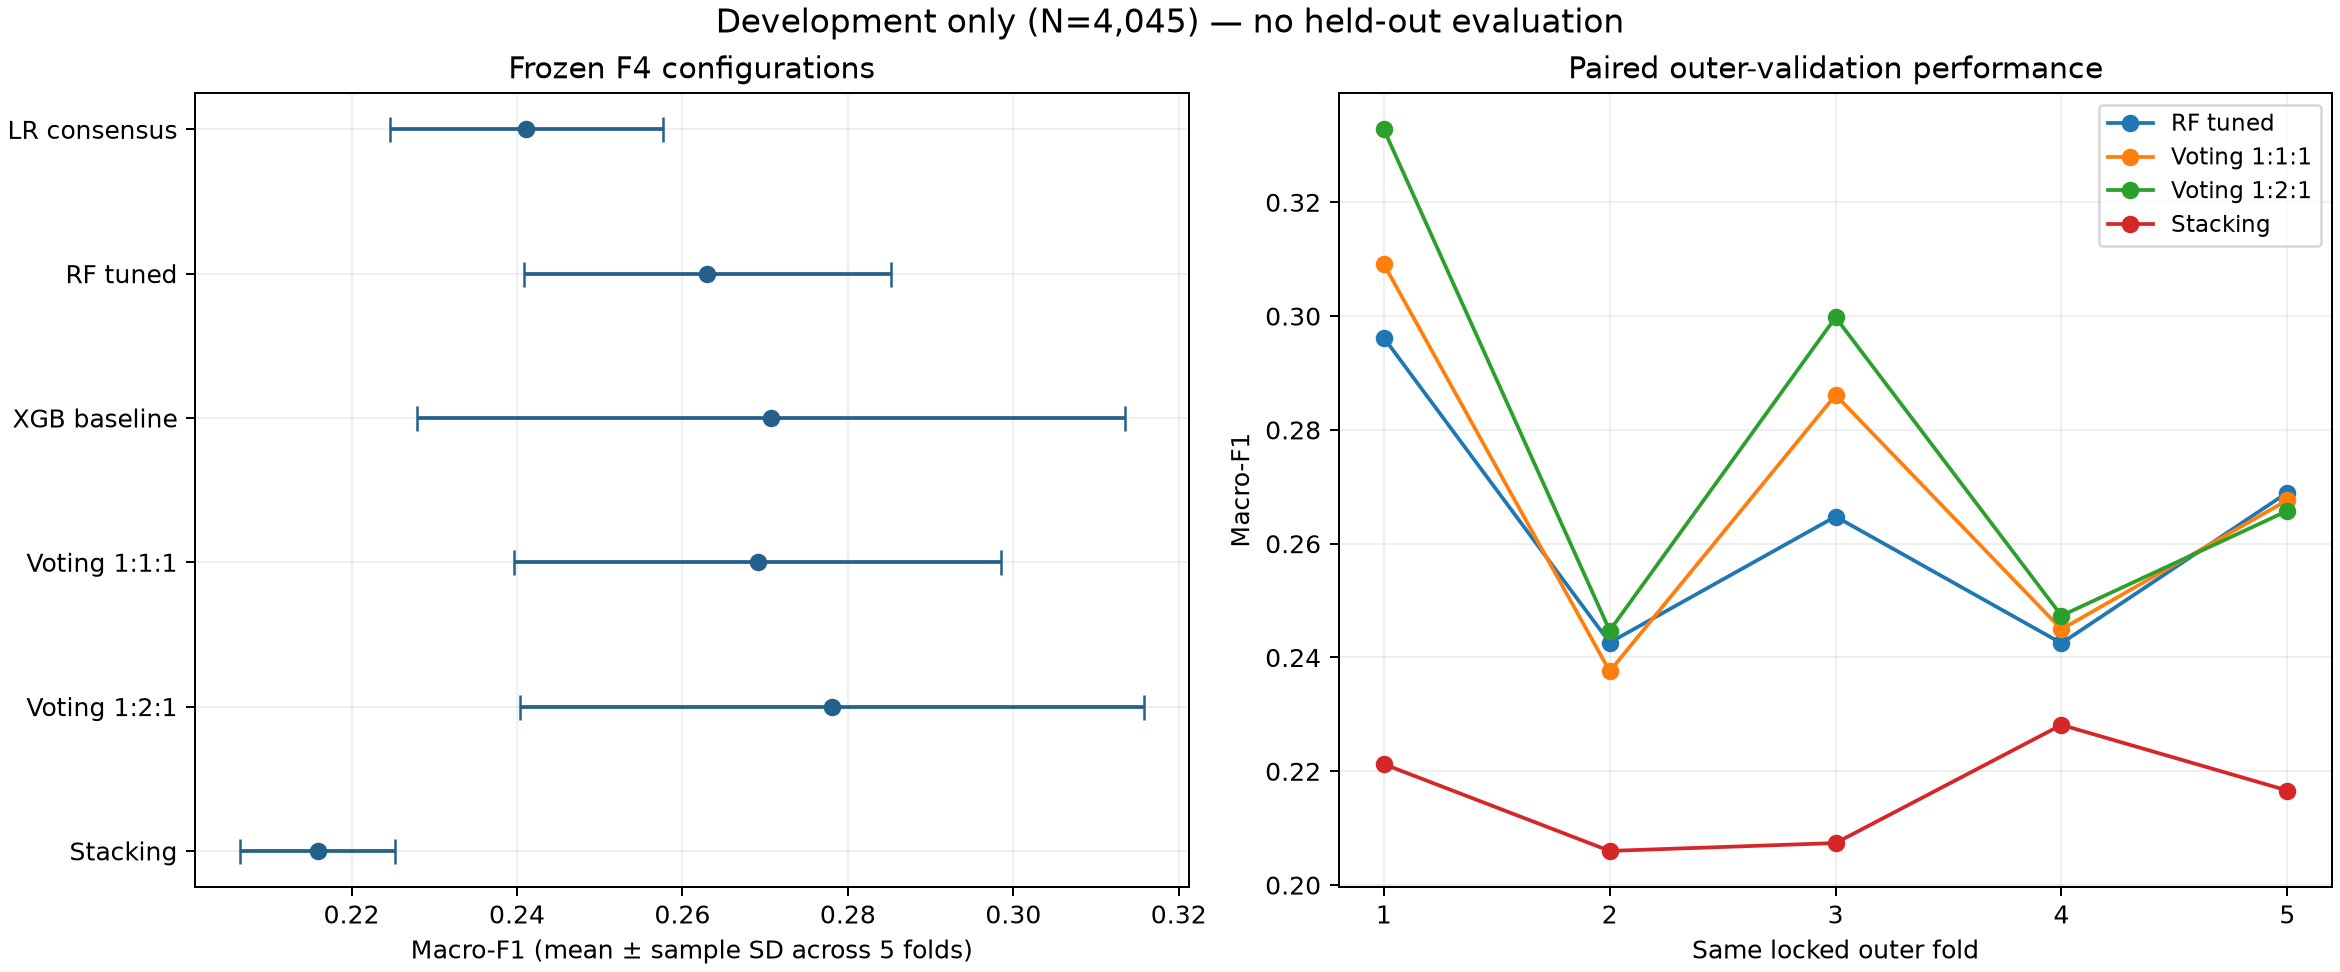
\includegraphics[width=0.85\textwidth]{figures/ensemble_comparison.png}
\label{fig:ensemble-comparison}
\end{figure}
\FloatBarrier

Theo tiêu chí thực nghiệm, một mô hình phức tạp hơn chỉ được ưu tiên nếu cải thiện Macro-F1 tối thiểu +0.01 một cách ổn định qua các folds. Cả Soft Voting và Stacking đều không đáp ứng tiêu chí này. Do đó, nghiên cứu giữ nguyên Frozen Random Forest làm mô hình cơ sở.

\section{Khảo sát độ chi tiết nhãn mục tiêu ($T_2 \to T_5$)}
\label{sec:target-granularity}

\subsection{Khảo sát biến thiên hiệu năng theo độ chi tiết nhãn}
Để trả lời câu hỏi nghiên cứu \textbf{RQ2}, nghiên cứu khảo sát sự thay đổi hiệu năng khi chuyển từ bài toán nhị phân ($T_2$) sang các mức độ chi tiết hơn ($T_3, T_4, T_5$) trên cùng mô hình Frozen Random Forest và không gian đặc trưng $F_4$ ($N = 4.045$).

Kết quả out-of-fold được trình bày trong Bảng \ref{tab:granularity-results}. Sự biến thiên được minh họa trong Hình \ref{fig:granularity-curves} và Hình \ref{fig:granularity-dist}.

\begin{table}{Hiệu năng mô hình Random Forest theo độ chi tiết nhãn mục tiêu ($T_2 \to T_5$) trên Legacy Development ($N = 4.045$)}
\centering
\footnotesize
\setlength{\tabcolsep}{3pt}
\label{tab:granularity-results}
\begin{tabularx}{\textwidth}{l c >{\centering\arraybackslash}X >{\centering\arraybackslash}X >{\centering\arraybackslash}X >{\centering\arraybackslash}X}
\toprule
\textbf{Nhiệm vụ} & \textbf{Số lớp} & \textbf{Độ chính xác (Acc)} & \textbf{Macro-F1 (Mean $\pm$ SD)} & \textbf{Balanced Acc} & \textbf{Weighted-F1} \\
\midrule
$T_2$ (Không vs Có) & 2 & 74.24\% $\pm$ 1.26\% & \textbf{0.6639 $\pm$ 0.0113} & \textbf{0.6659 $\pm$ 0.0122} & 0.7436 $\pm$ 0.0100 \\
$T_3$ ($C_0, C_1, C_2^+$) & 3 & 64.10\% $\pm$ 2.79\% & 0.4354 $\pm$ 0.0075 & 0.4667 $\pm$ 0.0101 & 0.6538 $\pm$ 0.0156 \\
$T_4$ ($C_0, C_1, C_2, C_{3+4}$) & 4 & 61.06\% $\pm$ 2.58\% & 0.3380 $\pm$ 0.0177 & 0.3661 $\pm$ 0.0202 & 0.6351 $\pm$ 0.0169 \\
$T_5$ (5 mức chuẩn PHQ-9) & 5 & 61.38\% $\pm$ 2.03\% & 0.2630 $\pm$ 0.0222 & 0.2805 $\pm$ 0.0199 & 0.6339 $\pm$ 0.0116 \\
\bottomrule
\end{tabularx}
\end{table}


\begin{figure}[htbp]{Biến thiên hiệu năng Macro-F1 và Balanced Accuracy từ bài toán nhị phân $T_2$ đến đa lớp $T_5$}
\centering
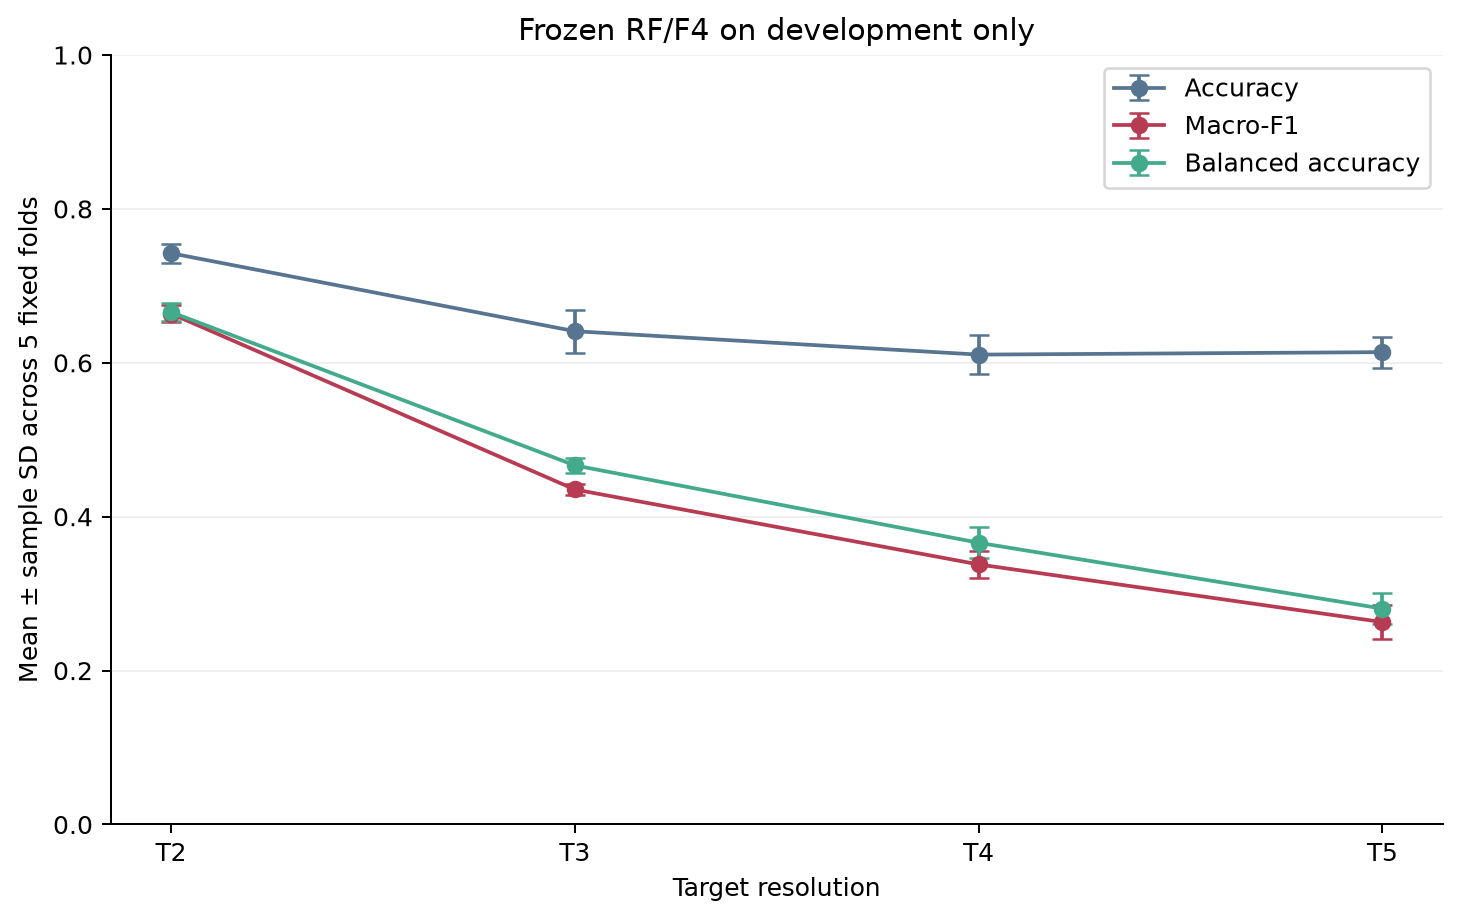
\includegraphics[width=0.85\textwidth]{figures/granularity_performance.png}
\label{fig:granularity-curves}
\end{figure}
\FloatBarrier

\begin{figure}[htbp]{Biến động cấu trúc phân bố các lớp khi tăng độ phân giải nhãn mục tiêu từ $T_2$ đến $T_5$}
\centering
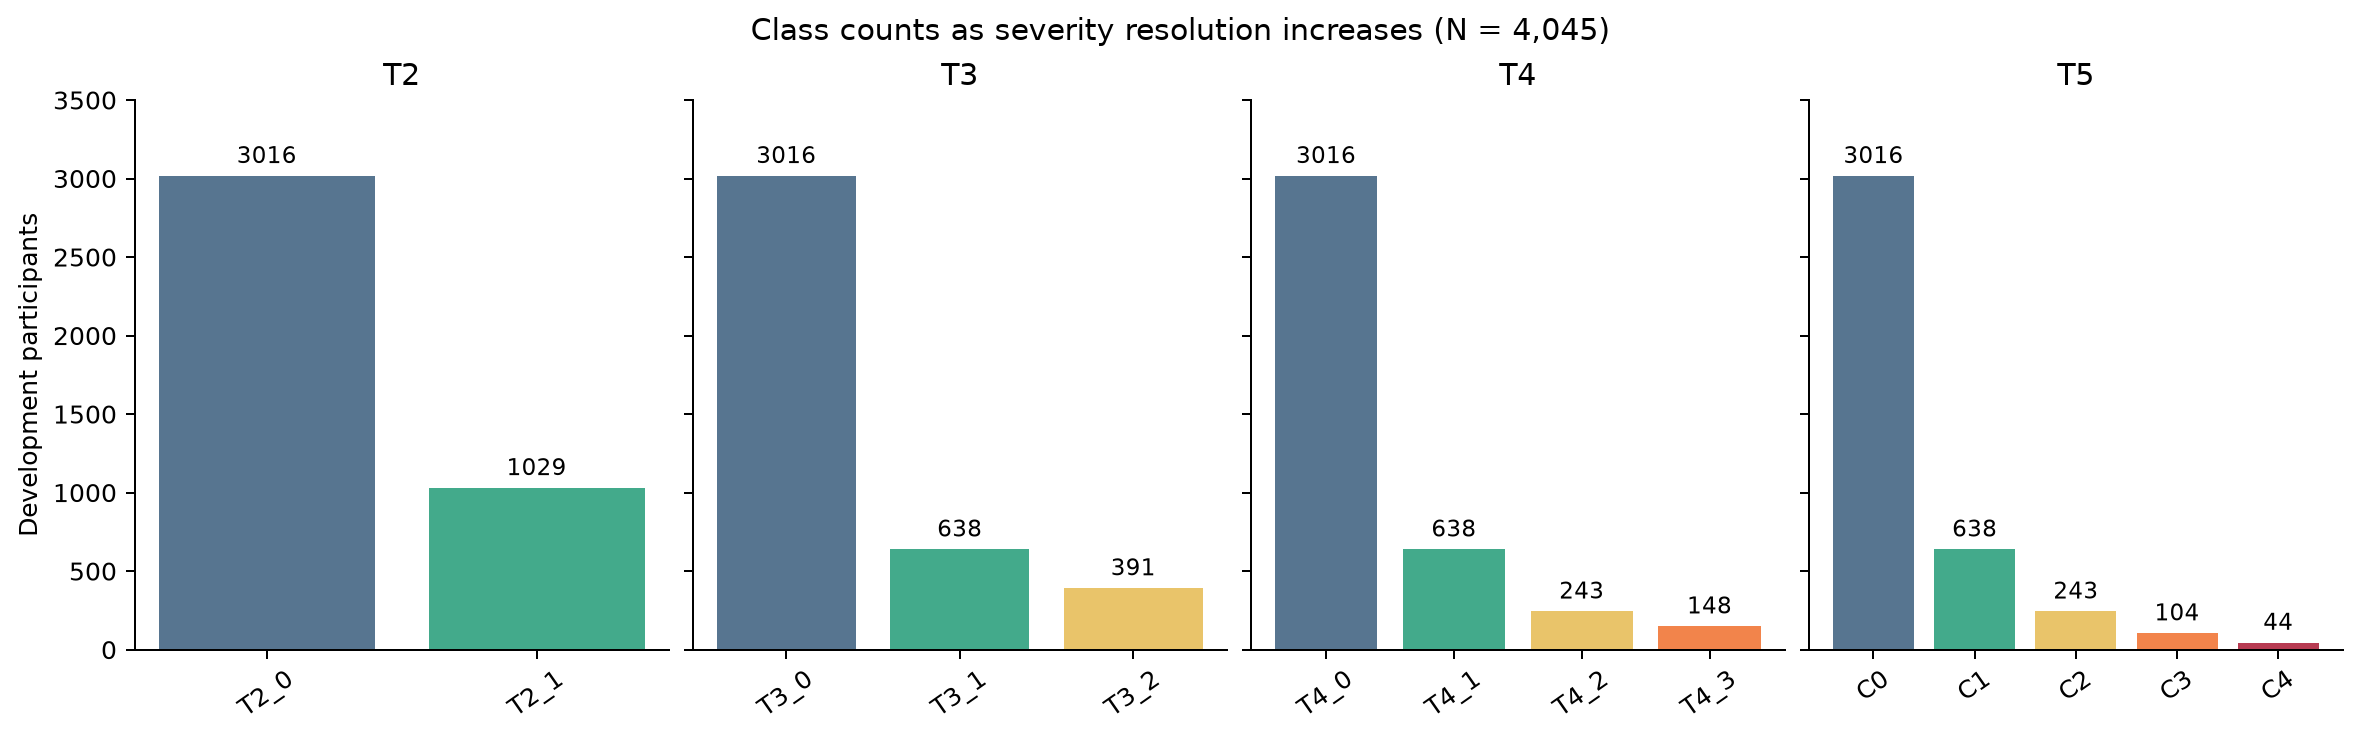
\includegraphics[width=0.85\textwidth]{figures/granularity_class_distribution.png}
\label{fig:granularity-dist}
\end{figure}
\FloatBarrier

\subsection{Phân tích biến thiên ranh giới và Ma trận nhầm lẫn $T_5$}
Từ Bảng \ref{tab:granularity-results}, mức độ thay đổi hiệu năng đáng chú ý nhất diễn ra tại bước chuyển từ $T_2$ sang $T_3$: Macro-F1 thay đổi từ \textbf{0.6639 sang 0.4354} (-34.4\%), và Balanced Accuracy từ \textbf{0.6659 sang 0.4667} (-29.9\%). Khi tiếp tục tăng độ chi tiết lên $T_4$ và $T_5$, Macro-F1 đạt lần lượt 0.3380 và 0.2630. Cần lưu ý rằng $T_2$ và $T_3$ có không gian nhãn mục tiêu khác nhau (2 lớp so với 3 lớp); do đó sự biến thiên này phản ánh độ phức tạp gia tăng khi mô hình phải phân định ranh giới giữa các nhóm triệu chứng liền kề.

Để phân tích chi tiết kết quả dự đoán của mô hình Random Forest trên 5 lớp phẳng $T_5$, ma trận nhầm lẫn $5 \times 5$ được trích xuất từ dữ liệu thực nghiệm out-of-fold ($N = 4.045$, nguồn từ \texttt{results/tables/granularity\_confusion\_matrices.csv}) và được thể hiện trong Hình \ref{fig:t5-confusion-matrix}:
\begin{itemize}
    \item \textbf{Lớp tối thiểu $C_0$ (3.016 mẫu):} 2.295 mẫu dự đoán đúng (Recall = 76.09\%), 385 mẫu nhầm sang $C_1$, 272 mẫu sang $C_2$, 55 mẫu sang $C_3$, 9 mẫu sang $C_4$.
    \item \textbf{Lớp nhẹ $C_1$ (638 mẫu):} Chỉ 101 mẫu dự đoán đúng (\textbf{Recall = 15.83\%}), trong khi có tới \textbf{344 mẫu (53.92\%) bị xếp sang $C_0$}. 149 mẫu nhầm sang $C_2$, 38 mẫu sang $C_3$, 6 mẫu sang $C_4$.
    \item \textbf{Lớp vừa $C_2$ (243 mẫu):} 67 mẫu đúng (Recall = 27.57\%), 73 mẫu nhầm sang $C_0$, 65 mẫu sang $C_1$, 30 mẫu sang $C_3$, 8 mẫu sang $C_4$.
    \item \textbf{Lớp nặng vừa $C_3$ (104 mẫu):} 19 mẫu đúng (Recall = 18.27\%), 24 mẫu nhầm sang $C_0$, 19 mẫu sang $C_1$, 40 mẫu sang $C_2$, 2 mẫu sang $C_4$.
    \item \textbf{Lớp nặng $C_4$ (44 mẫu):} \textbf{Chỉ 1 mẫu được dự đoán đúng (Recall = 2.27\%)}; 11 mẫu (25.0\%) bị xếp sang $C_0$, 9 mẫu sang $C_1$, 15 mẫu sang $C_2$, và 8 mẫu sang $C_3$.
\end{itemize}

\begin{figure}[htbp]{Ma trận nhầm lẫn của Random Forest trên bài toán 5 mức độ $T_5$ (Out-of-Fold, $N = 4.045$)}
\centering
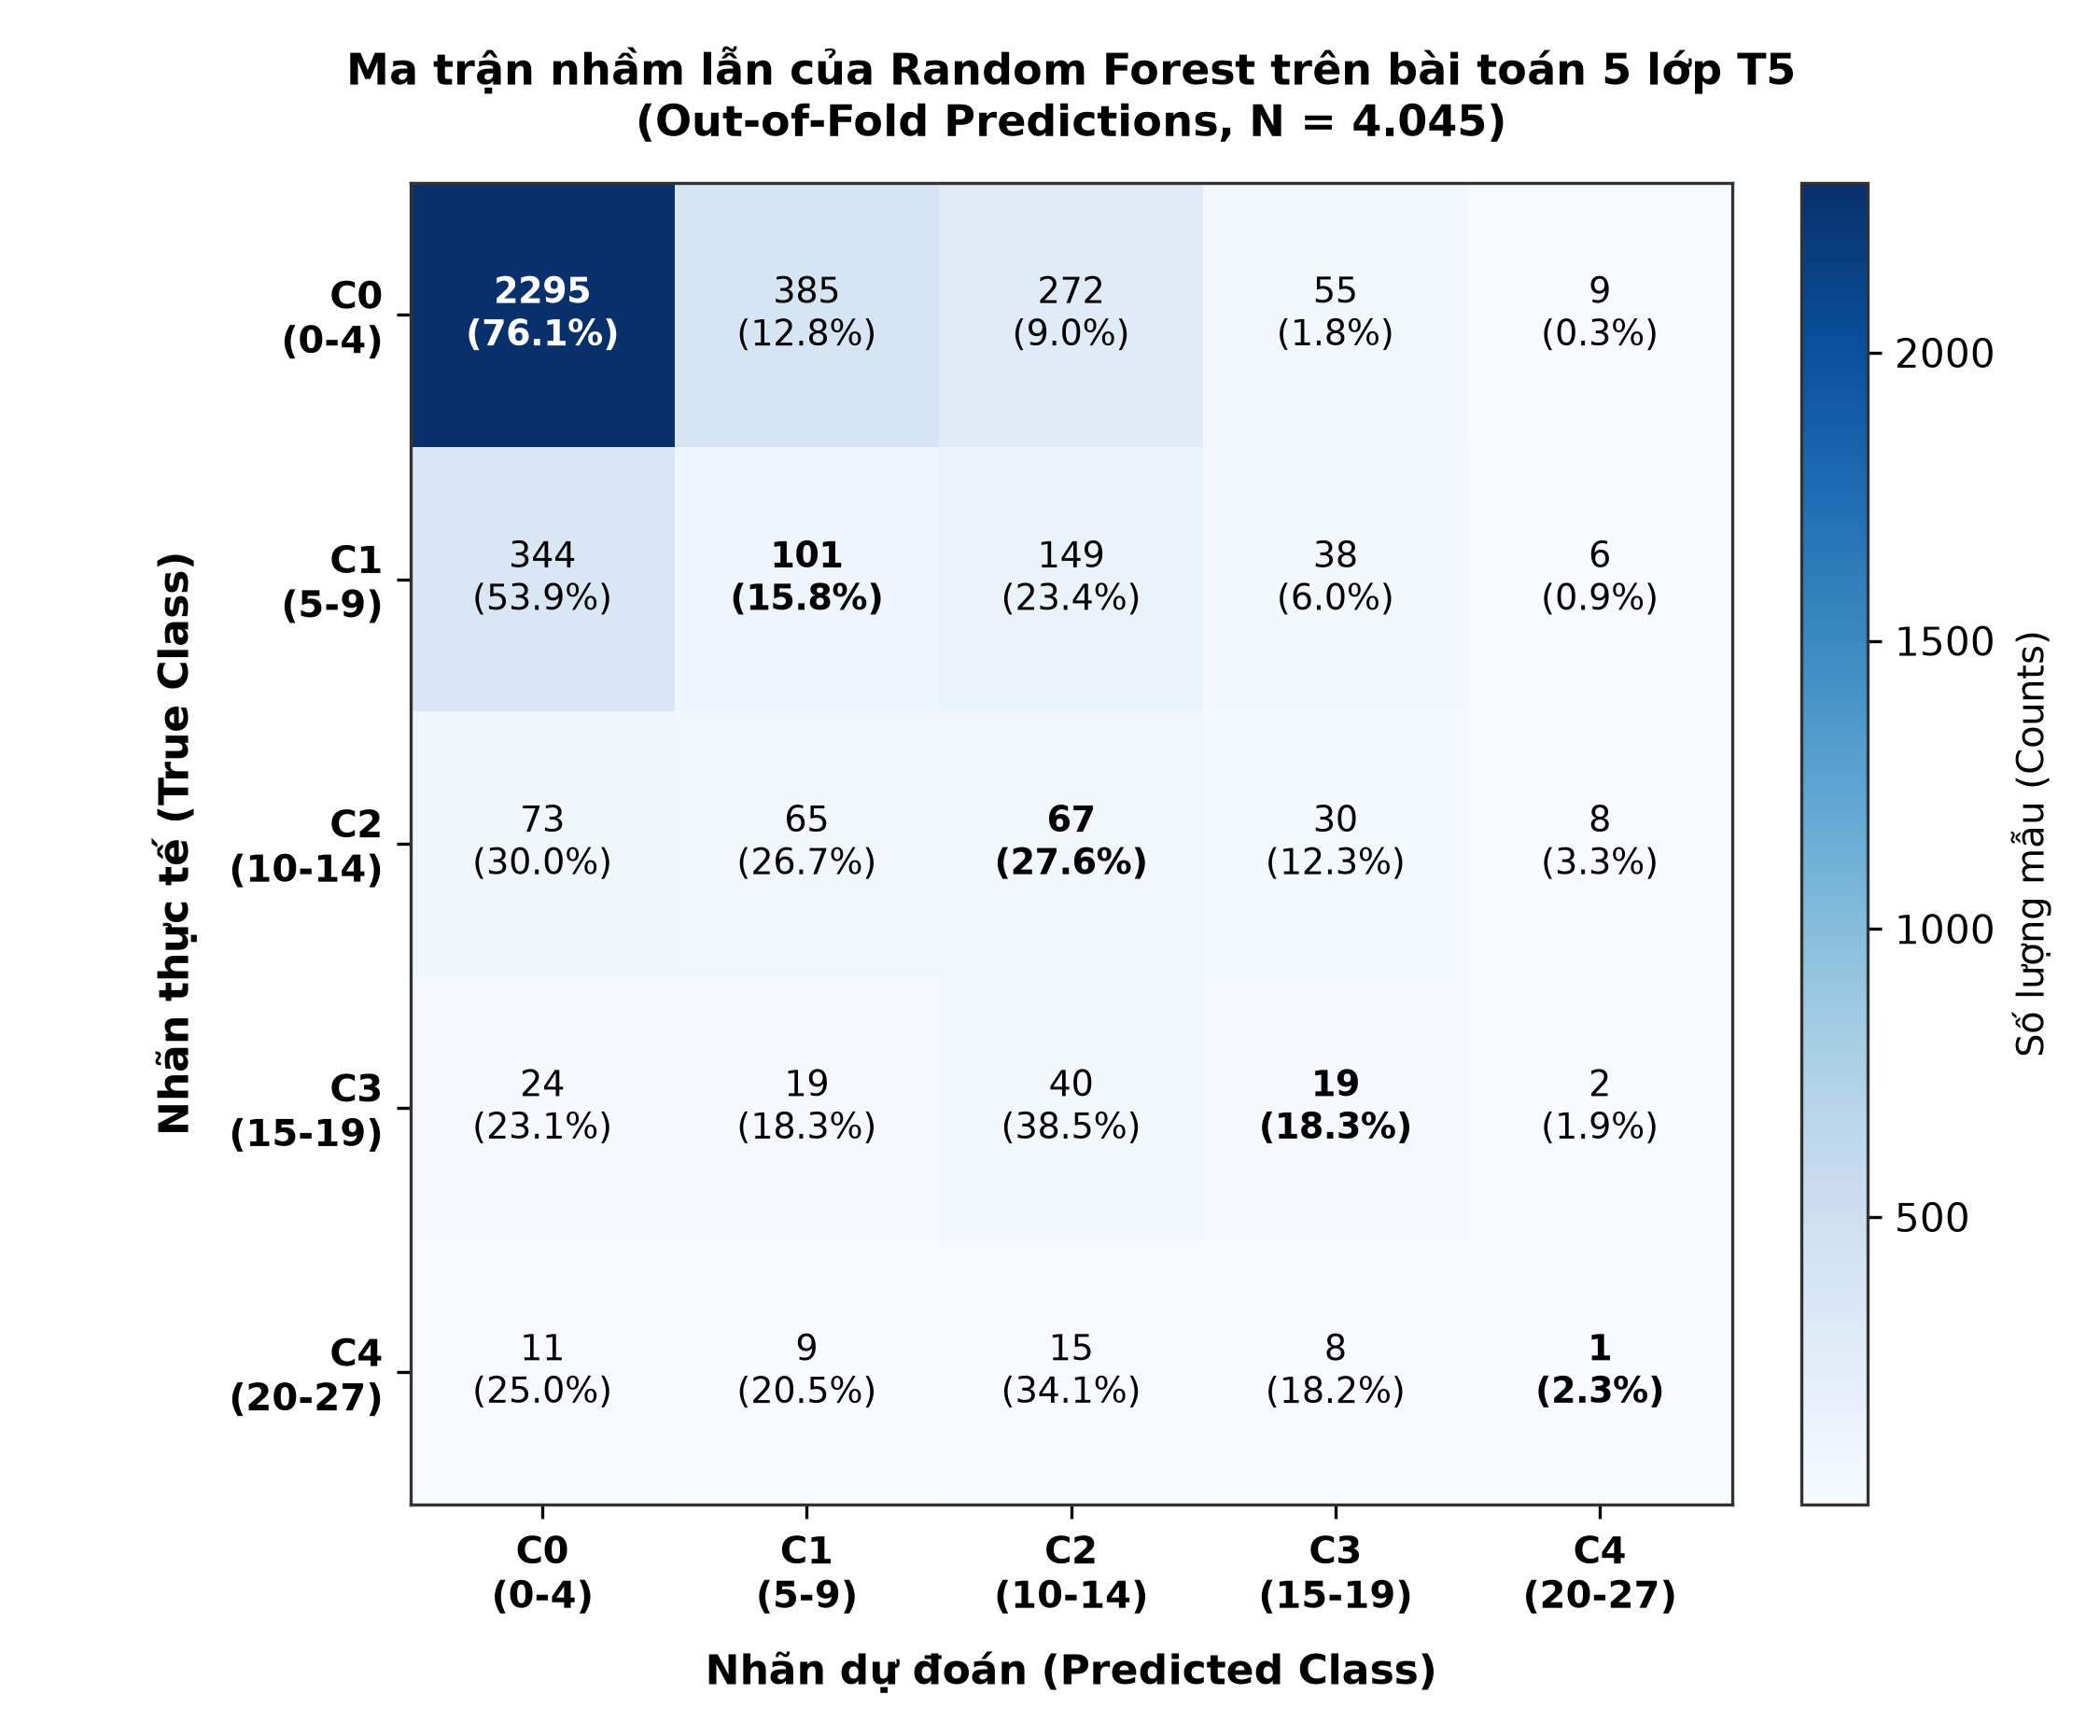
\includegraphics[width=0.75\textwidth]{figures/granularity_t5_confusion_matrix.png}
\label{fig:t5-confusion-matrix}
\end{figure}
\FloatBarrier

Ma trận nhầm lẫn $5 \times 5$ cho thấy: mô hình phân loại phẳng trên dữ liệu sinh lý ngoại vi có tỷ lệ nhận diện thấp ở lớp $C_4$ do cỡ mẫu rất nhỏ (44 mẫu trong tổng 4.045 quan sát), đồng thời có sự nhầm lẫn đáng kể giữa lớp $C_0$ và $C_1$. Các quan sát này đặt ra yêu cầu phải phân tích sâu hơn về đặc tính phân phối của các biến số đầu vào, đồng thời cung cấp cơ sở thực nghiệm quan trọng để nghiên cứu khảo sát thêm các hướng tiếp cận phân loại phân cấp và thứ bậc trên không gian 3 nhóm $T_3$.

\section{Phân tích đặc tính dữ liệu: Mức độ tương quan và chồng lấn phân phối đặc trưng}
\label{sec:phan-tich-chong-lan}

Để tìm hiểu các nguyên nhân dẫn đến đặc tính phân loại quan sát được ở Mục \ref{sec:target-granularity}, nghiên cứu tiến hành phân tích phân phối và mối liên hệ giữa các biến số với điểm số PHQ-9.

\subsection{Tương quan giữa các chỉ số cận lâm sàng và điểm PHQ-9}
Mức độ liên hệ giữa các biến đầu vào và tổng điểm PHQ-9 được thể hiện trong Hình \ref{fig:correlation-matrix}:
\begin{itemize}
    \item \textbf{Biến liên tục (Panel a):} Hệ số tương quan hạng Spearman ($\rho$) trích xuất từ dữ liệu thực nghiệm cho thấy nồng độ Albumin huyết thanh ($\rho = -0.164$), tỷ lệ thu nhập trên chuẩn nghèo PIR ($\rho = -0.159$) và thời lượng giấc ngủ ($\rho = -0.139$) có tương quan âm nhẹ với điểm PHQ-9; trong khi chỉ số khối cơ thể BMI ($\rho = +0.114$), chu vi vòng eo ($\rho = +0.095$), nhịp tim khi nghỉ ($\rho = +0.085$) và thời gian ngồi tĩnh tại ($\rho = +0.043$) có tương quan dương nhẹ.
    \item \textbf{Biến phân loại (Panel b):} Hệ số liên hệ Cramer's V ghi nhận tự đánh giá sức khỏe chung (HUQ010) có mức độ liên hệ cao nhất ($V = 0.195$), tiếp theo là giới tính ($V = 0.144$), hoạt động thể lực giải trí (PAQ665, $V = 0.125$), tiền sử tăng huyết áp (BPQ020, $V = 0.109$) và tiền sử đái tháo đường (DIQ010, $V = 0.100$).
\end{itemize}
Tất cả các hệ số tương quan và liên hệ đều ở mức khiêm tốn ($|\rho| \le 0.17$, $V \le 0.20$), chứng minh rằng không có bất kỳ biến sinh lý hay lâm sàng đơn lẻ nào mang tính quyết định để phân tách rạch ròi các mức độ triệu chứng.

\begin{figure}[htbp]{Mức độ tương quan và liên hệ giữa các đặc trưng đầu vào với điểm số PHQ-9: (a) Hệ số tương quan hạng Spearman $\rho$ của các biến liên tục; (b) Hệ số liên hệ Cramer's V của các biến phân loại}
\centering
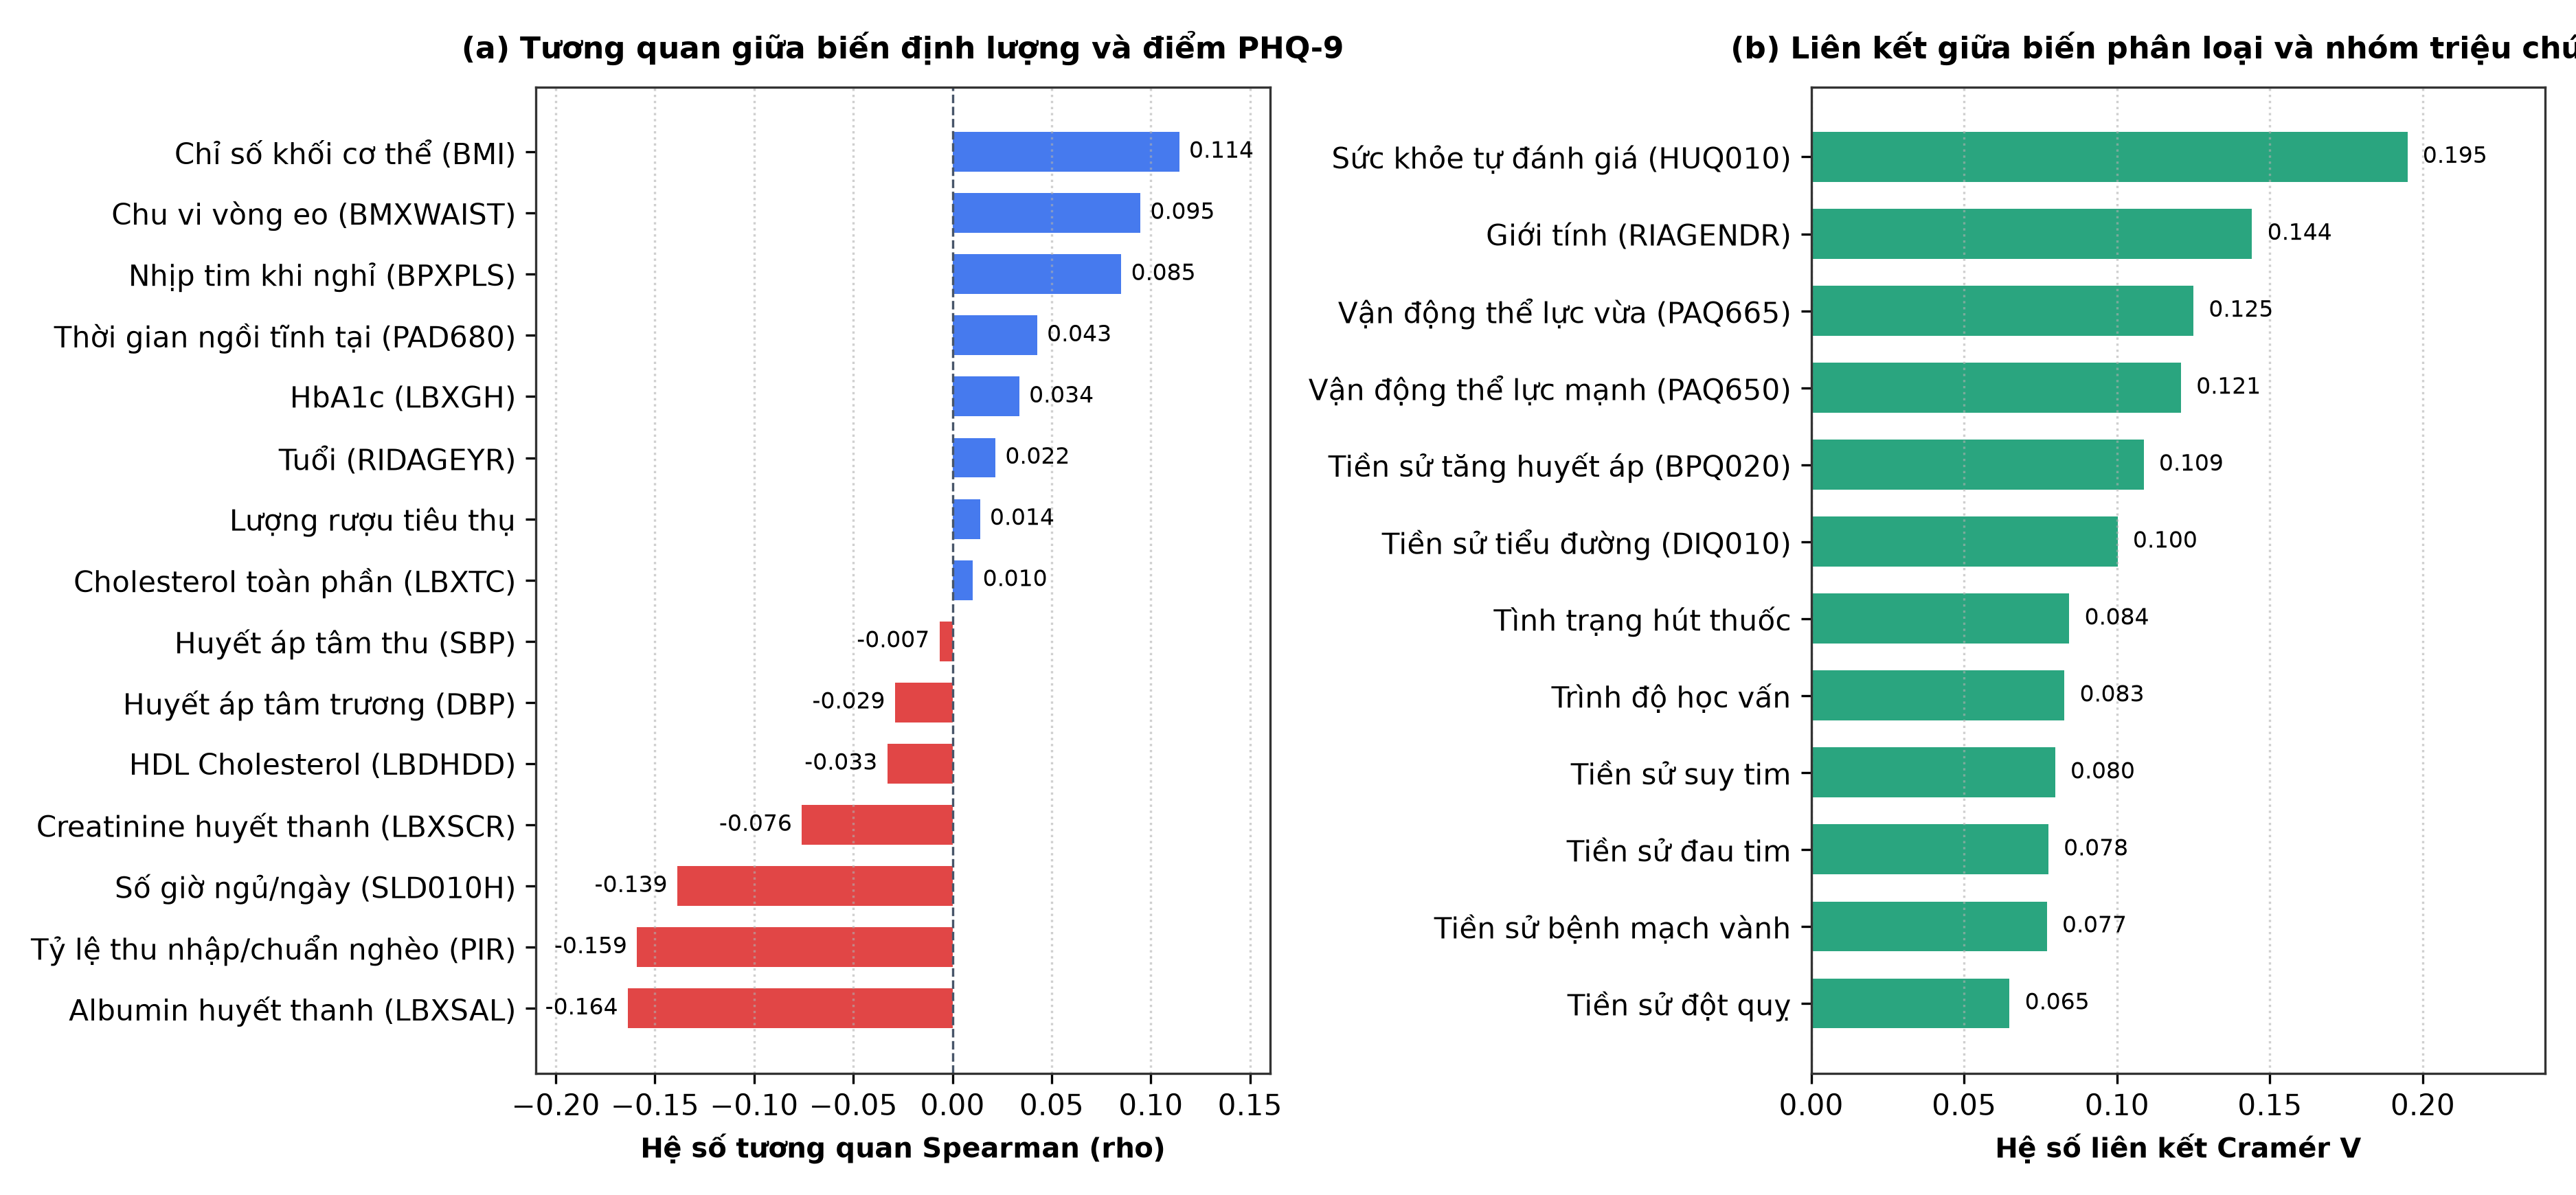
\includegraphics[width=0.92\textwidth]{figures/correlation_matrix.png}
\label{fig:correlation-matrix}
\end{figure}
\FloatBarrier

\subsection{Phân tích biểu đồ hộp và hình chiếu PCA}
Hình \ref{fig:overlap-boxplots} thể hiện phân bố giá trị của 6 chỉ số đặc trưng liên tục tiêu biểu (BMI, PIR, Giờ ngủ, Albumin, Nhịp tim, Thời gian ngồi tĩnh tại) qua các mức độ PHQ-9. Khoảng tứ phân vị (IQR) và trung vị của nhóm triệu chứng tối thiểu ($C_0$) và nhóm triệu chứng nhẹ ($C_1$) gần như trùng khớp nhau trên hầu hết các biến số (chẳng hạn trung vị BMI ở $C_0$ là 28.1 $\text{kg/m}^2$ so với 29.5 $\text{kg/m}^2$ ở $C_1$; Albumin ở $C_0$ là 43.0 g/L so với 42.0 g/L ở $C_1$; thời lượng ngủ trung vị cùng là 7.0 giờ). Sự phân tách chỉ bắt đầu thể hiện nhẹ ở nhóm triệu chứng nặng ($C_4$), tuy nhiên độ phân tán nội nhóm vẫn rất lớn.

\begin{figure}[htbp]{Biểu đồ hộp thể hiện sự tương đồng và chồng lấn phân phối của 6 biến sinh lý chính qua các mức độ PHQ-9}
\centering
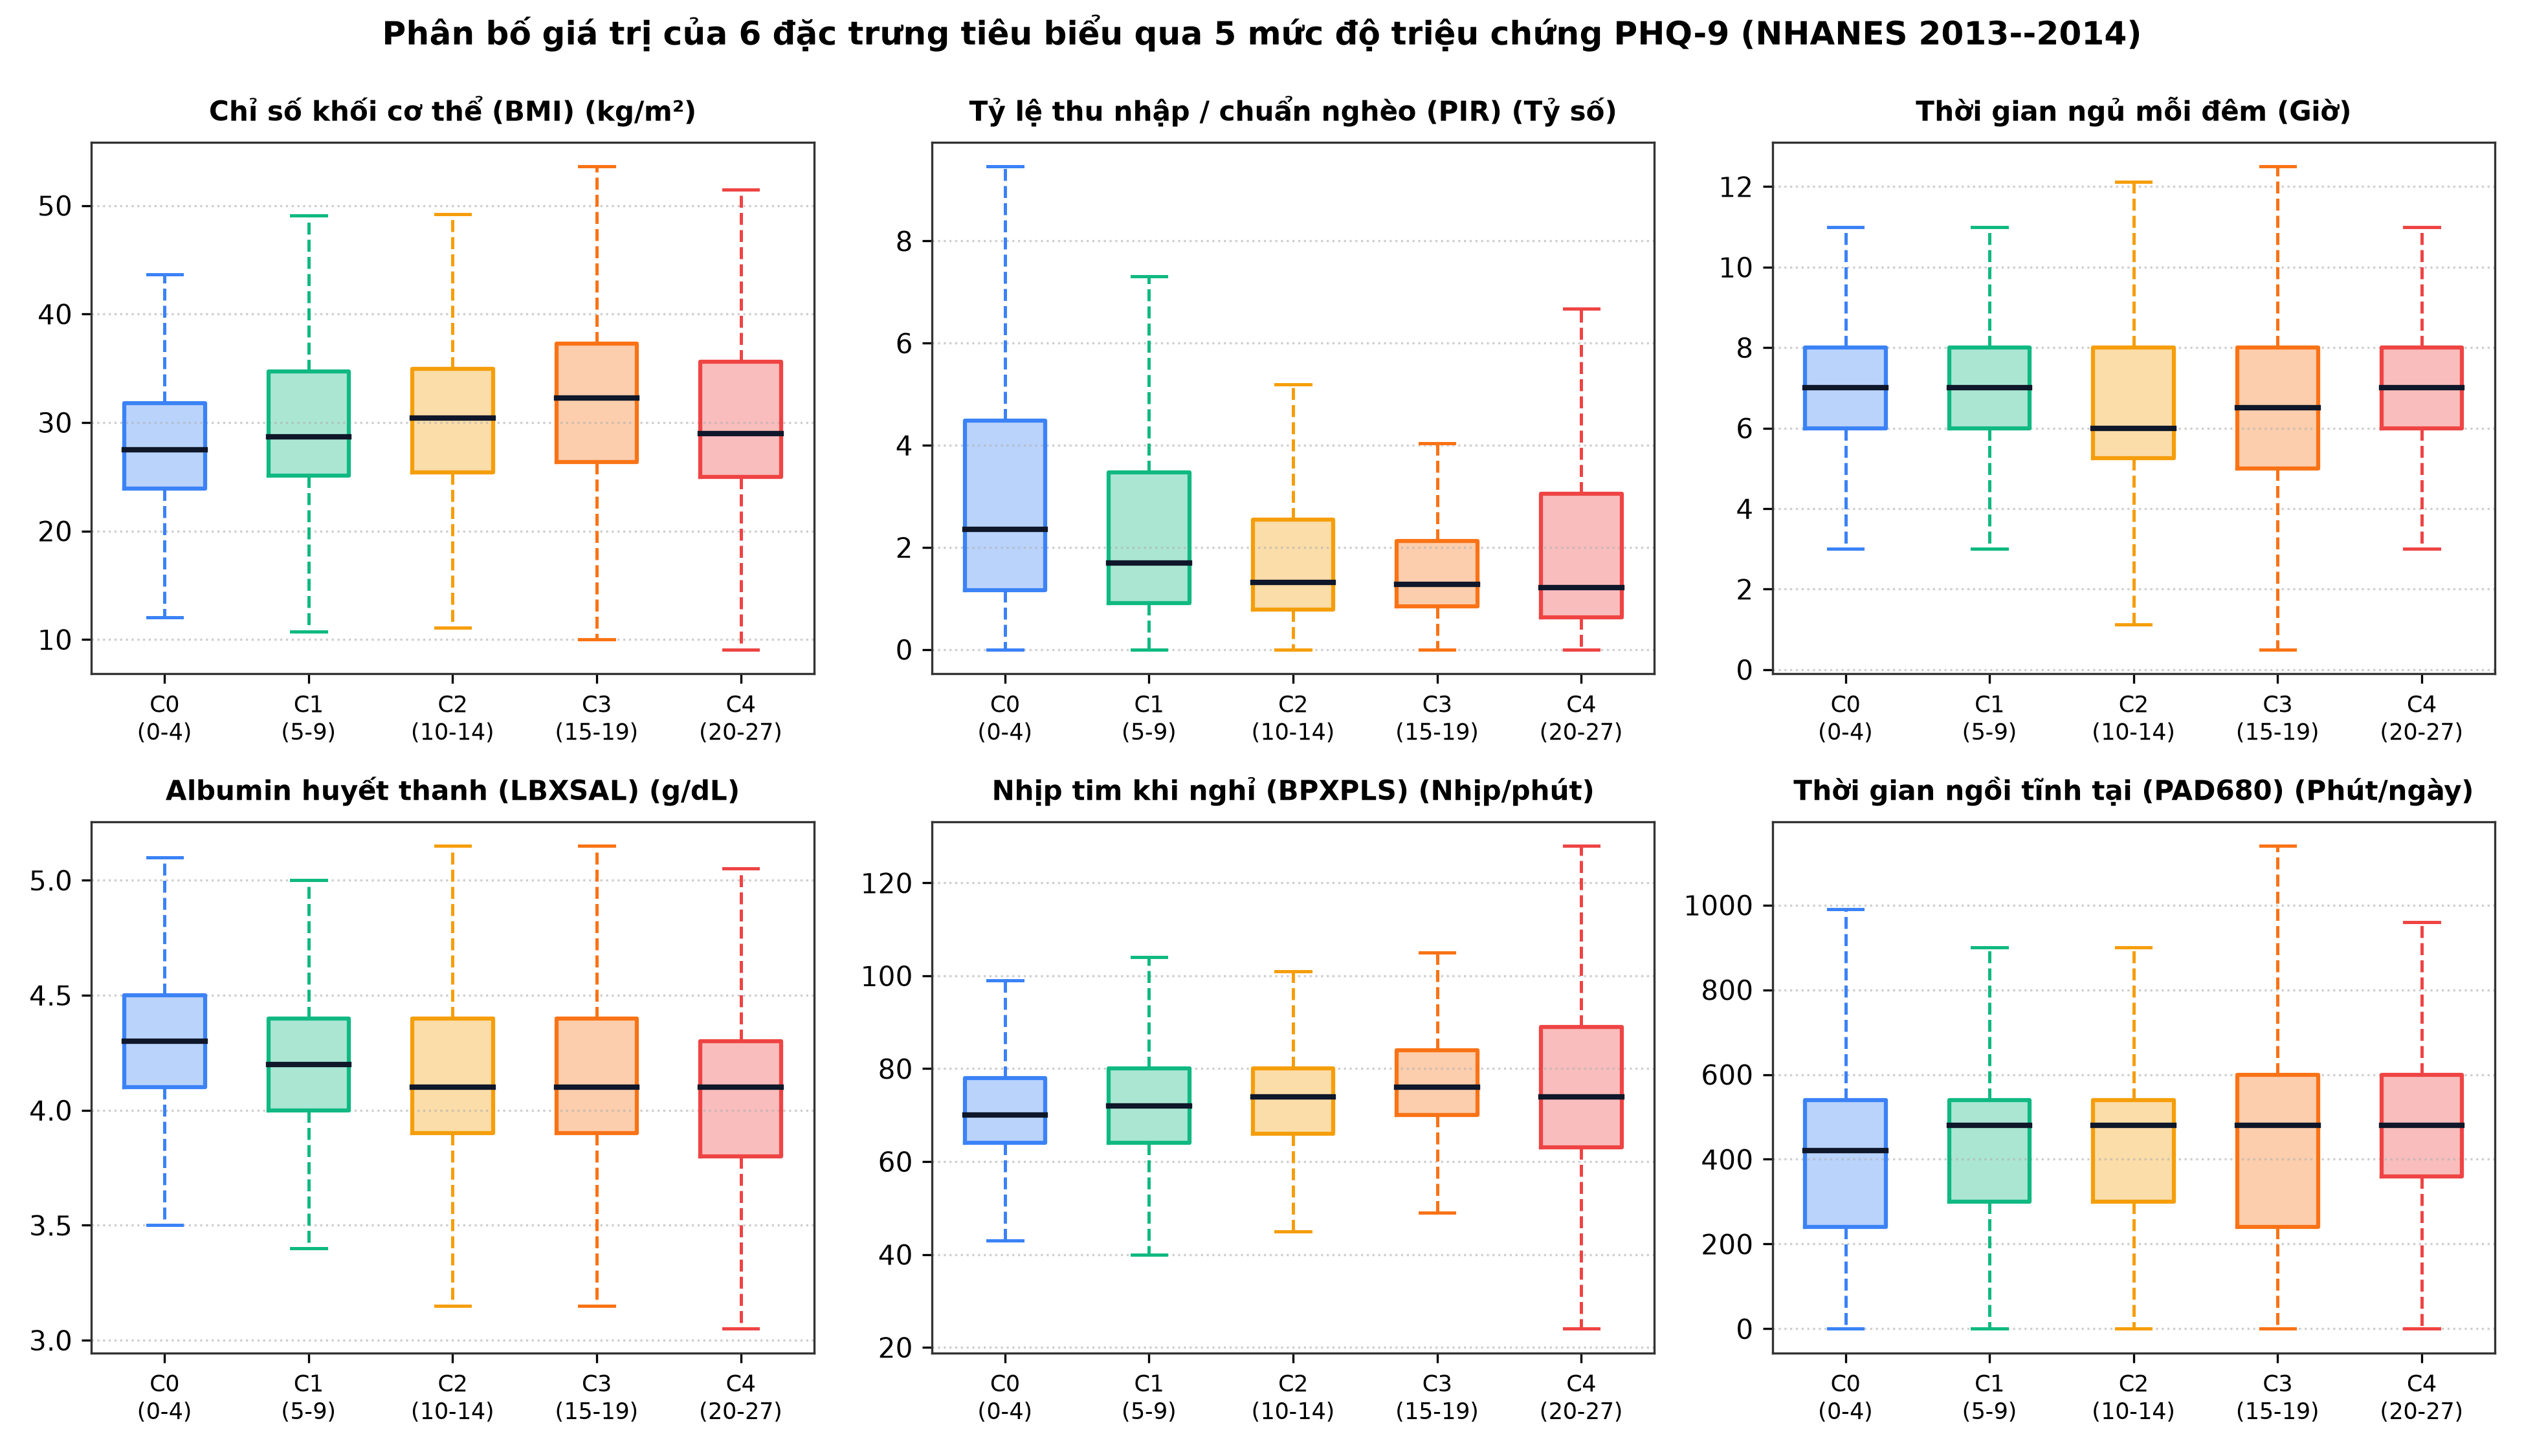
\includegraphics[width=0.92\textwidth]{figures/overlap_numerical_boxplots.png}
\label{fig:overlap-boxplots}
\end{figure}
\FloatBarrier

Khi chiếu không gian đặc trưng xuống mặt phẳng hai thành phần chính đầu tiên (PCA 2D, Hình \ref{fig:pca-overlap}), hai thành phần PC1 (12.3\%) và PC2 (8.8\%) giải thích tổng cộng 21.1\% phương sai dữ liệu. Cả trên không gian 5 mức độ $T_5$ (Panel a) lẫn không gian 3 nhóm $T_3$ (Panel b), đám mây điểm của nhóm $C_1$ lọt hoàn toàn vào bên trong đường bao mật độ của nhóm $C_0$. Nhóm nặng $C_4$ cũng không hình thành cụm tách biệt mà nằm phân tán rải rác.

Cần lưu ý rằng PCA là một phép chiếu tuyến tính hai chiều, không đại diện cho toàn bộ các tương tác phi tuyến phức tạp trong không gian đa chiều gốc. Dù vậy, hình chiếu PCA 2D trực quan hóa rõ nét hiện tượng chồng lấn phân phối sinh lý, giúp giải thích vì sao các mô hình học máy thường xuyên nhầm lẫn giữa các nhóm triệu chứng liền kề.

\begin{figure}[htbp]{Hình chiếu PCA 2D của không gian đặc trưng thể hiện sự chồng lấn phân phối: (a) Trên 5 mức độ $T_5$; (b) Trên 3 nhóm $T_3$}
\centering
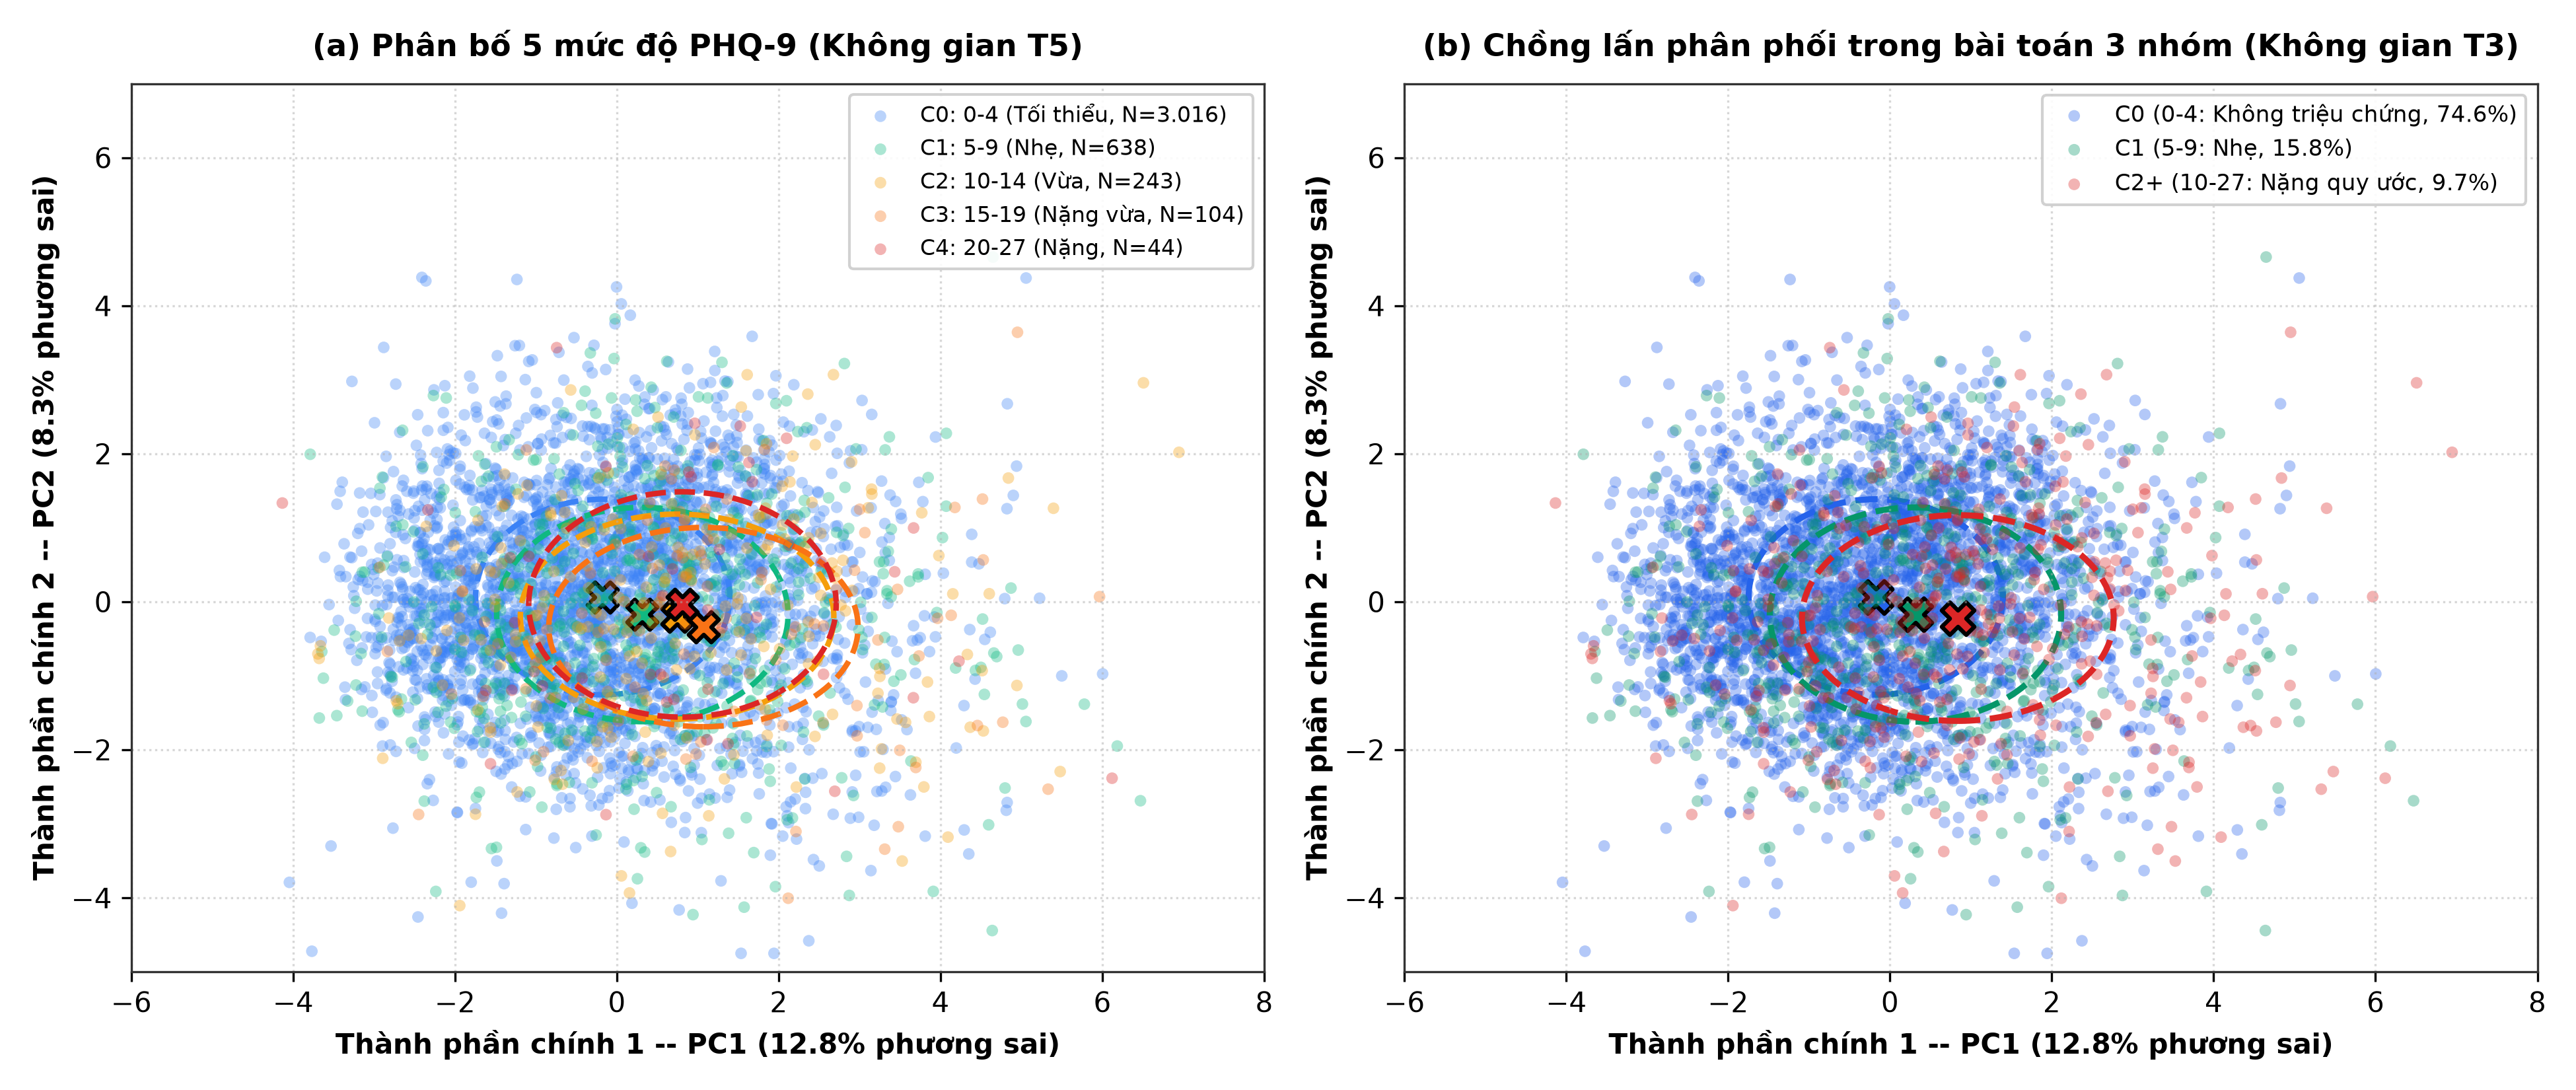
\includegraphics[width=0.92\textwidth]{figures/overlap_pca_C0_C4.png}
\label{fig:pca-overlap}
\end{figure}
\FloatBarrier

\section{Thử nghiệm mở rộng dữ liệu đa chu kỳ NHANES}
\label{sec:multicycle-results}

Để trả lời câu hỏi nghiên cứu \textbf{RQ3}, nghiên cứu tiến hành kiểm định trên tập dữ liệu gộp đa chu kỳ Pooled NHANES 2011--2016 ($N = 14.581$, tăng gấp 3.6 lần cỡ mẫu) với không gian 31 đặc trưng hài hòa ($F_{4\_\text{common31}}$).

Kết quả so sánh giữa chu kỳ đơn lẻ (Branch A, $N = 5.054$), tập dữ liệu gộp 3 chu kỳ (Branch B, $N = 14.581$) và kiểm định ngoại suy theo thời gian (Branch D, $N = 4.888$) qua các mức độ chi tiết nhãn ($T_2 \to T_5$) được thể hiện trong Hình \ref{fig:multicycle-cohort-comparison}.

\begin{figure}[htbp]{So sánh Macro-F1 và Balanced Accuracy theo độ chi tiết nhãn giữa chu kỳ đơn lẻ (Branch A), tập dữ liệu gộp (Branch B) và kiểm định thời gian (Branch D)}
\centering
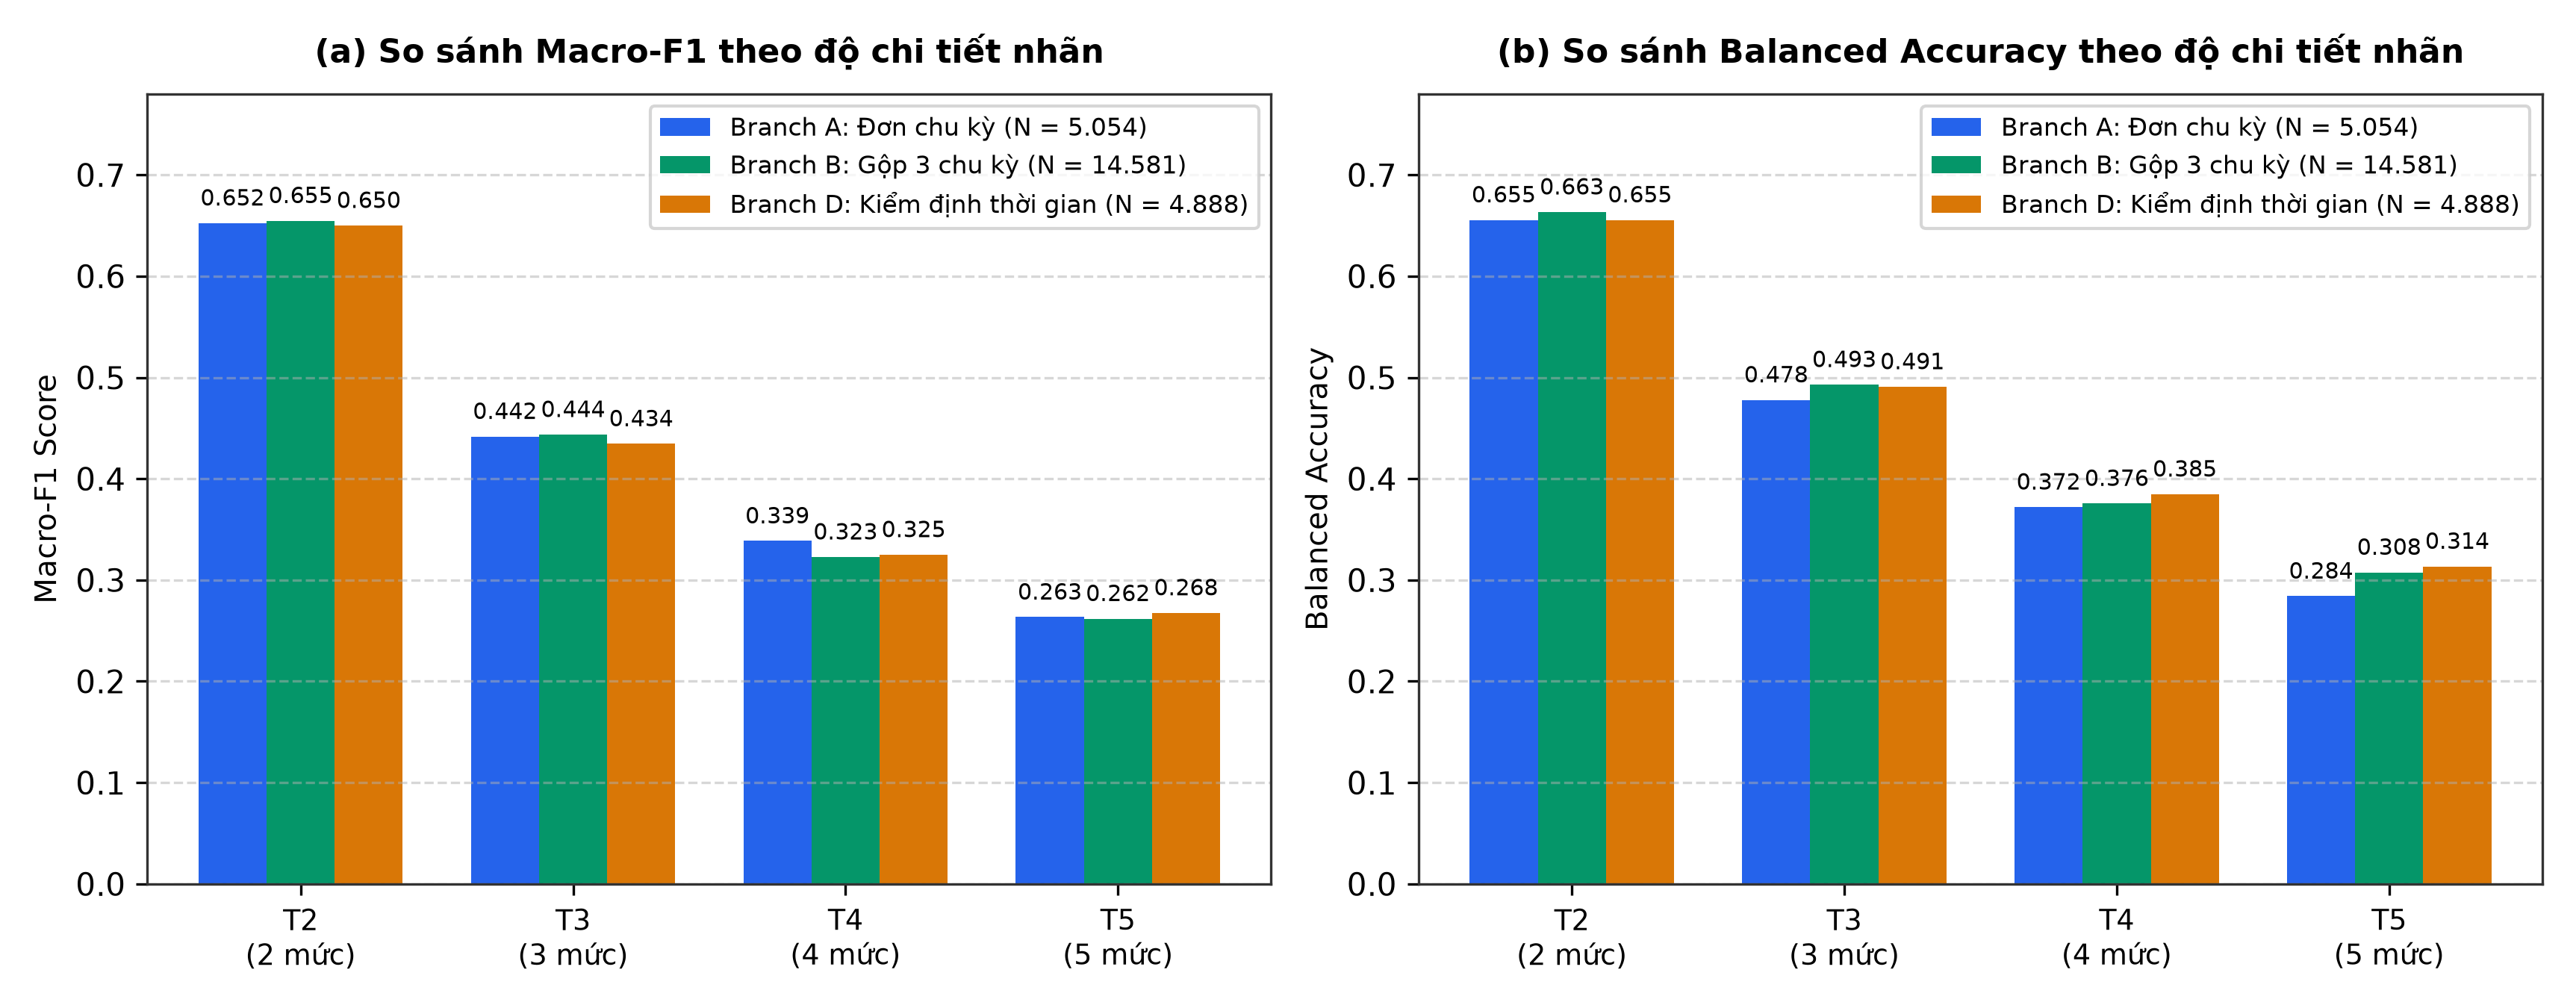
\includegraphics[width=\textwidth]{figures/multicycle_cohort_comparison.png}
\label{fig:multicycle-cohort-comparison}
\end{figure}
\FloatBarrier

Kết quả thực nghiệm cho thấy:
\begin{itemize}
    \item Việc tăng cỡ mẫu lên $14.581$ đối tượng giúp cải thiện nhẹ Balanced Accuracy trên nhiệm vụ 5 mức $T_5$ (tăng từ 0.2841 lên 0.3076).
    \item Tuy nhiên, Macro-F1 trên $T_5$ không có sự cải thiện rõ rệt (0.2634 ở Branch A so với 0.2619 ở Branch B).
\end{itemize}
Kết quả này cho thấy khi dữ liệu gặp hiện tượng chồng lấn phân phối giữa các nhóm triệu chứng, việc chỉ gia tăng cỡ mẫu đơn thuần mà không bổ sung thêm các chiều đặc trưng có độ đặc hiệu cao hơn khó có thể tạo ra bước nhảy vọt về hiệu năng phân loại trên bài toán 5 mức.

\section{Mở rộng khảo sát: Kết nối từ bài toán đa mức $T_5$ sang phân loại phân cấp và thứ bậc $T_3$}
\label{sec:chuyen-dich-t5-t3}

Các chuỗi thực nghiệm trên không gian 5 lớp $T_5$ đã mang lại nhiều hiểu biết có giá trị về đặc tính dữ liệu và hành vi của các mô hình học máy:
\begin{enumerate}
    \item \textbf{Đóng góp tích cực của các nhóm đặc trưng:} Việc mở rộng từ các chỉ số xét nghiệm và thể chất đơn thuần ($F_1$) sang không gian tích hợp tiền sử bệnh lý, lối sống và nhân khẩu học ($F_4$) nâng Macro-F1 từ 0.1900 lên 0.2707, chứng minh các yếu tố hành vi và nhân khẩu học cung cấp tín hiệu bổ trợ quan trọng cho phân tầng nguy cơ.
    \item \textbf{Đặc tính phân phối sinh lý ngoại vi:} Phân tích tương quan hạng Spearman, liên hệ Cramer's V và biểu đồ hình chiếu PCA 2D đã chỉ ra rằng các chỉ số sinh lý ngoại vi giữa nhóm triệu chứng tối thiểu ($C_0$) và triệu chứng nhẹ ($C_1$) có độ tương đồng và chồng lấn phân phối rất lớn. Đây là đặc điểm khách quan của các biến số dạng bảng trích xuất từ khảo sát sức khỏe cộng đồng.
    \item \textbf{Khảo sát quy mô mẫu:} Việc mở rộng cỡ mẫu lên 14.581 quan sát qua 3 chu kỳ NHANES giúp ổn định Balanced Accuracy (tăng từ 0.2841 lên 0.3076) nhưng không làm tăng đáng kể Macro-F1 trên $T_5$, khẳng định rằng đặc tính phân tách của bài toán phụ thuộc chủ yếu vào mức độ đặc hiệu của tập biến số hơn là số lượng mẫu quan sát.
\end{enumerate}

Trong bối cảnh sàng lọc sức khỏe tâm thần ban đầu, bên cạnh bài toán phân loại chi tiết 5 mức độ, một nhu cầu thực tế thường được quan tâm là phân tầng đối tượng theo hai bước ra quyết định rõ ràng:
\begin{itemize}
    \item \textit{Bước 1 (Nhận diện triệu chứng):} Phân biệt giữa người có triệu chứng tối thiểu ($C_0$, điểm 0--4) và người có biểu hiện triệu chứng cần lưu ý ($C_{12}$, điểm 5--27).
    \item \textit{Bước 2 (Phân tầng mức độ):} Trong nhóm người có triệu chứng, phân biệt giữa mức nhẹ ($C_1$, điểm 5--9) và mức nặng theo quy ước nghiên cứu ($C_2^+$, điểm 10--27).
\end{itemize}

Do đó, các phát hiện thực nghiệm trên $T_5$ đóng vai trò là cơ sở khoa học để nghiên cứu \textbf{mở rộng khảo sát sang bài toán 3 nhóm ($T_3$)} và đánh giá có hệ thống 8 cấu hình mô hình thực nghiệm ($E_0 \to E_7$) đại diện cho các hướng tiếp cận phẳng, phân cấp cứng, phân cấp mềm kết hợp chi phí Bayes và phân loại thứ bậc. Cần nhấn mạnh rằng $T_3$ và $T_5$ là hai bài toán phân loại độc lập với không gian nhãn và mục tiêu ứng dụng khác nhau; việc khảo sát song song cả hai bài toán giúp cung cấp bức tranh hoàn chỉnh về đặc điểm của các mô hình học máy trên dữ liệu sinh lý dạng bảng.

\begin{figure}[htbp]{Tổng hợp kết quả khảo sát trên hai hướng thực nghiệm: Phân loại đa mức $T_5$ và các hướng mô hình hóa trên $T_3$}
\centering
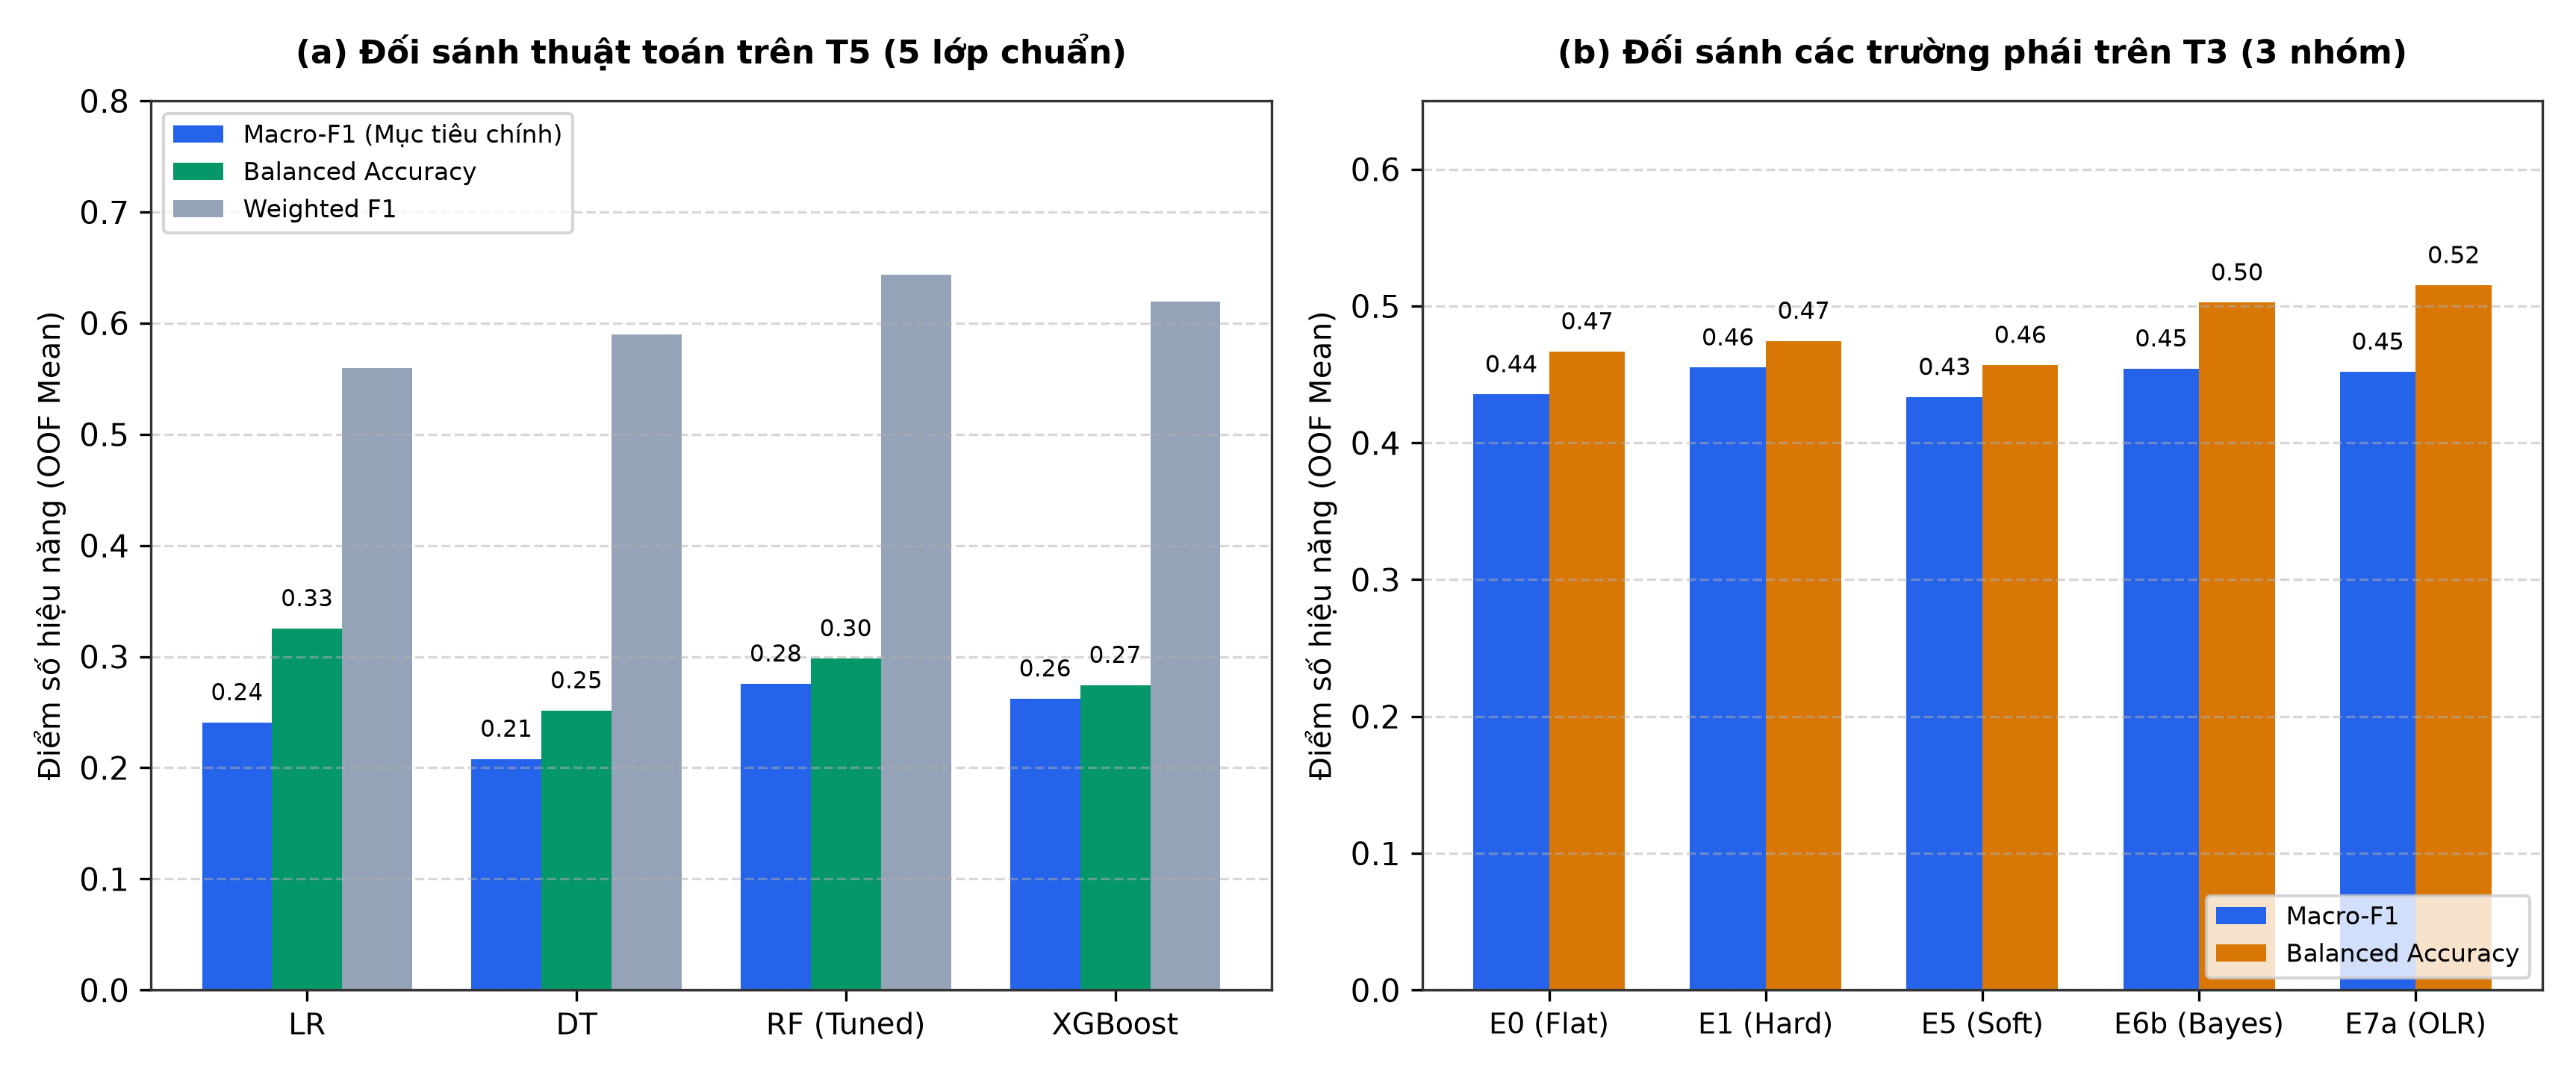
\includegraphics[width=\textwidth]{figures/fig4_algorithm_comparison_t5_t3.png}
\label{fig:algo-comparison-t5-t3}
\end{figure}
\FloatBarrier

\section{Khảo sát các hướng tiếp cận mô hình hóa trên không gian 3 nhóm ($T_3$): Đánh giá $E_0 \to E_7$}
\label{sec:khao-sat-e0-e7}

Trên không gian 3 nhóm ($T_3$: $C_0, C_1, C_2^+$), nghiên cứu khảo sát có hệ thống 8 cấu hình mô hình thực nghiệm ($E_0 \to E_7$) trên tập phát triển Legacy ($N = 4.045$).

\subsection{Kết quả các cấu hình phân cấp cứng ($E_1 \to E_3$)}
Kiến trúc phân cấp cứng chia bài toán thành hai bộ phân loại nhị phân nối tiếp: Stage 1 ($M_1$) sàng lọc $C_0$ vs $C_{12}$; Stage 2 ($M_2$) phân tầng $C_1$ vs $C_2^+$.
\begin{itemize}
    \item \textbf{Cơ chế huấn luyện in-fold:} Bộ phân loại Stage 1 được huấn luyện trên toàn bộ dữ liệu huấn luyện của fold. Bộ phân loại Stage 2 được huấn luyện \textbf{chỉ trên các mẫu trong fold có nhãn thật $\text{PHQ-9} \ge 5$} ($N = 1.029$ ca trên toàn bộ tập phát triển).
    \item \textbf{Cơ chế suy luận ngoài mẫu:} Nếu $M_1$ dự đoán một mẫu là $C_0$, mẫu được gán nhãn $C_0$ ngay lập tức. Chỉ các mẫu được dự đoán là $C_{12}$ mới được chuyển sang Stage 2.
\end{itemize}

Kết quả thực nghiệm out-of-fold của các mô hình phân cấp cứng được trình bày trong Bảng \ref{tab:hard-hierarchical-results}.

\begin{table}{So sánh hiệu năng giữa Flat Classification và Hard Hierarchical trên nhiệm vụ $T_3$ ($N = 4.045$)}
\centering
\footnotesize
\setlength{\tabcolsep}{3pt}
\label{tab:hard-hierarchical-results}
\begin{tabularx}{\textwidth}{l >{\centering\arraybackslash}X >{\centering\arraybackslash}X >{\centering\arraybackslash}X >{\centering\arraybackslash}X >{\centering\arraybackslash}X >{\centering\arraybackslash}X}
\toprule
\textbf{Mô hình} & \textbf{Macro-F1 (Mean $\pm$ SD)} & \textbf{BalAcc} & \textbf{Accuracy} & \textbf{Recall $C_1$} & \textbf{Recall $C_2^+$} & \textbf{Bỏ sót $C_2^+ \to C_0$} \\
\midrule
$E_0$ (Flat RF)       & 0.4354 $\pm$ 0.0075 & 0.4667 & 64.10\% & 16.29\% & 47.32\% & 108 ca \\
$E_1$ (Hard RF--RF)   & 0.4550 $\pm$ 0.0056 & 0.4745 & 68.08\% & 16.46\% & 43.74\% & 120 ca \\
$E_2$ (Hard Tuned)    & \textbf{0.4586 $\pm$ 0.0124} & 0.4745 & 65.32\% & \textbf{25.69\%} & 39.63\% & \textbf{98 ca} \\
$E_3a$ (Hard RF--LR)  & 0.4567 $\pm$ 0.0271 & \textbf{0.4964} & \textbf{68.43\%} & 11.75\% & \textbf{55.00\%} & 120 ca \\
$E_3b$ (Hard RF--XGB) & 0.4575 $\pm$ 0.0182 & 0.4790 & 68.23\% & 16.77\% & 44.76\% & 120 ca \\
\bottomrule
\end{tabularx}

\vspace{0.15cm}
\raggedright
\scriptsize
\textit{Ghi chú:} Số ca bỏ sót $C_2^+ \to C_0$ là số lượng tổng hợp từ toàn bộ dự đoán ngoài mẫu (pooled out-of-fold, $N = 4.045$).
\end{table}


\textbf{Phân tích kết quả phân cấp cứng:}
\begin{enumerate}
    \item \textbf{Cải thiện Macro-F1:} Cấu hình phân cấp cứng $E_1$ (Hard RF--RF) đạt Macro-F1 = \textbf{0.4550 $\pm$ 0.0056}, cải thiện so với mô hình phẳng $E_0$ (0.4354). Cấu hình tối ưu siêu tham số $E_2$ (Hard RF--RF Tuned) nâng Macro-F1 lên mức cao nhất trong nhóm khảo sát là \textbf{0.4586 $\pm$ 0.0124}.
    \item \textbf{Đặc điểm lan truyền sai số và tỷ lệ bỏ sót ca nặng:} Trong mô hình $E_1$, có \textbf{120 ca nặng ($C_2^+$) bị Stage 1 dự đoán nhầm thành $C_0$} (tương đương 30.69\% tổng số 391 ca nặng). Khi đã bị Stage 1 gán nhãn $C_0$, các ca này kết thúc luồng dự đoán và không được Stage 2 tiếp cận. Cấu hình tối ưu siêu tham số $E_2$ giảm số ca này xuống còn \textbf{98 ca}. Con số này phản ánh đặc tính cơ học của định tuyến cứng: quyết định loại trừ ở giai đoạn 1 mang tính một chiều và không thể đảo ngược ở giai đoạn 2.
\end{enumerate}

\subsection{Kết quả các cấu hình phân cấp mềm và Quyết định nhạy chi phí ($E_4 \to E_6$)}
Nhằm linh hoạt điều chỉnh quy tắc quyết định và tận dụng phân phối xác suất liên tục giữa hai giai đoạn, các mô hình phân cấp mềm ($E_4, E_5$) kết hợp phân phối xác suất qua công thức xác suất toàn phần. Kết quả được trình bày trong Bảng \ref{tab:soft-cost-results}.

\begin{table}{Hiệu năng mô hình Soft Hierarchical và Quyết định Nhạy chi phí trên nhiệm vụ $T_3$ ($N = 4.045$)}
\centering
\footnotesize
\setlength{\tabcolsep}{3pt}
\label{tab:soft-cost-results}
\begin{tabularx}{\textwidth}{l >{\centering\arraybackslash}X >{\centering\arraybackslash}X >{\centering\arraybackslash}X >{\centering\arraybackslash}X >{\centering\arraybackslash}X >{\centering\arraybackslash}X >{\centering\arraybackslash}X}
\toprule
\textbf{Mô hình} & \textbf{Macro-F1} \newline \textbf{(Mean $\pm$ SD)} & \textbf{BalAcc} & \textbf{Accuracy} & \textbf{Recall $C_1$} & \textbf{Recall $C_2^+$} & \textbf{Bỏ sót} \newline \textbf{$C_2^+ \to C_0$} & \textbf{Báo động} \newline \textbf{$C_0 \to C_2^+$} \\
\midrule
$E_4$ (Soft RF--RF) & 0.4206 $\pm$ 0.0104 & 0.4309 & \textbf{73.75\%} & 5.18\% & 30.19\% & 227 ca & \textbf{139 ca} \\
$E_5$ (Soft RF--LR) & 0.4270 $\pm$ 0.0118 & 0.4506 & 73.37\% & 3.45\% & 39.13\% & 211 ca & 176 ca \\
$E_{6a}$ (Soft Cost RF--RF) & \textbf{0.4535 $\pm$ 0.0149} & 0.4904 & 56.91\% & \textbf{40.92\%} & 44.25\% & \textbf{62 ca} & 215 ca \\
$E_{6b}$ (Soft Cost RF--LR) & 0.4521 $\pm$ 0.0190 & \textbf{0.5025} & 56.84\% & 34.64\% & \textbf{54.23\%} & \textbf{62 ca} & 294 ca \\
\bottomrule
\end{tabularx}

\vspace{0.15cm}
\raggedright
\scriptsize
\textit{Ghi chú:} Macro-F1, BalAcc, Accuracy và Recall là trung bình qua 5 folds. Số ca bỏ sót và báo động là số lượng tổng hợp từ toàn bộ dự đoán ngoài mẫu (pooled out-of-fold, $N = 4.045$).
\end{table}


Để chủ động kiểm soát tỷ lệ bỏ sót ca nặng, cấu hình tối ưu chi phí Bayes $E_{6b}$ (Soft Cost RF--LR với ma trận chi phí $M_1$, đặt mức phạt bỏ sót ca nặng $\mathbf{C}(2, 0) = 3.0$) đưa hàm rủi ro kỳ vọng vào quy tắc quyết định. Kết quả thực nghiệm: $E_{6b}$ đạt Balanced Accuracy là \textbf{0.5025 $\pm$ 0.0163} và Macro-F1 = \textbf{0.4521 $\pm$ 0.0190}, đồng thời giảm số ca nặng bị bỏ sót thành bình thường ($C_2^+ \to C_0$) từ 120 ca ($E_1$) xuống còn \textbf{62 ca} (Hình \ref{fig:confusion-error-analysis}a), tương đương mức giảm \textbf{48.33\%} (tỷ lệ bỏ sót giảm từ 30.69\% xuống 15.86\%). Khi áp dụng ma trận phạt cao hơn $M_2$ ($\mathbf{C}(2, 0) = 5.0$), số ca bỏ sót giảm tiếp xuống còn \textbf{19 ca} (giảm 84.17\%), và với $M_3$ ($\mathbf{C}(2, 0) = 8.0$) chỉ còn \textbf{7 ca} (giảm 94.17\%), đổi lại số lượng báo động nhầm từ lớp bình thường tăng lên tương ứng.

\begin{figure}[htbp]{(a) Số ca nặng bị phân loại nhầm thành bình thường ($C_2^+ \to C_0$) và (b) So sánh Recall từng lớp giữa $E_1, E_{6b}$ và $E_{7a}$}
\centering
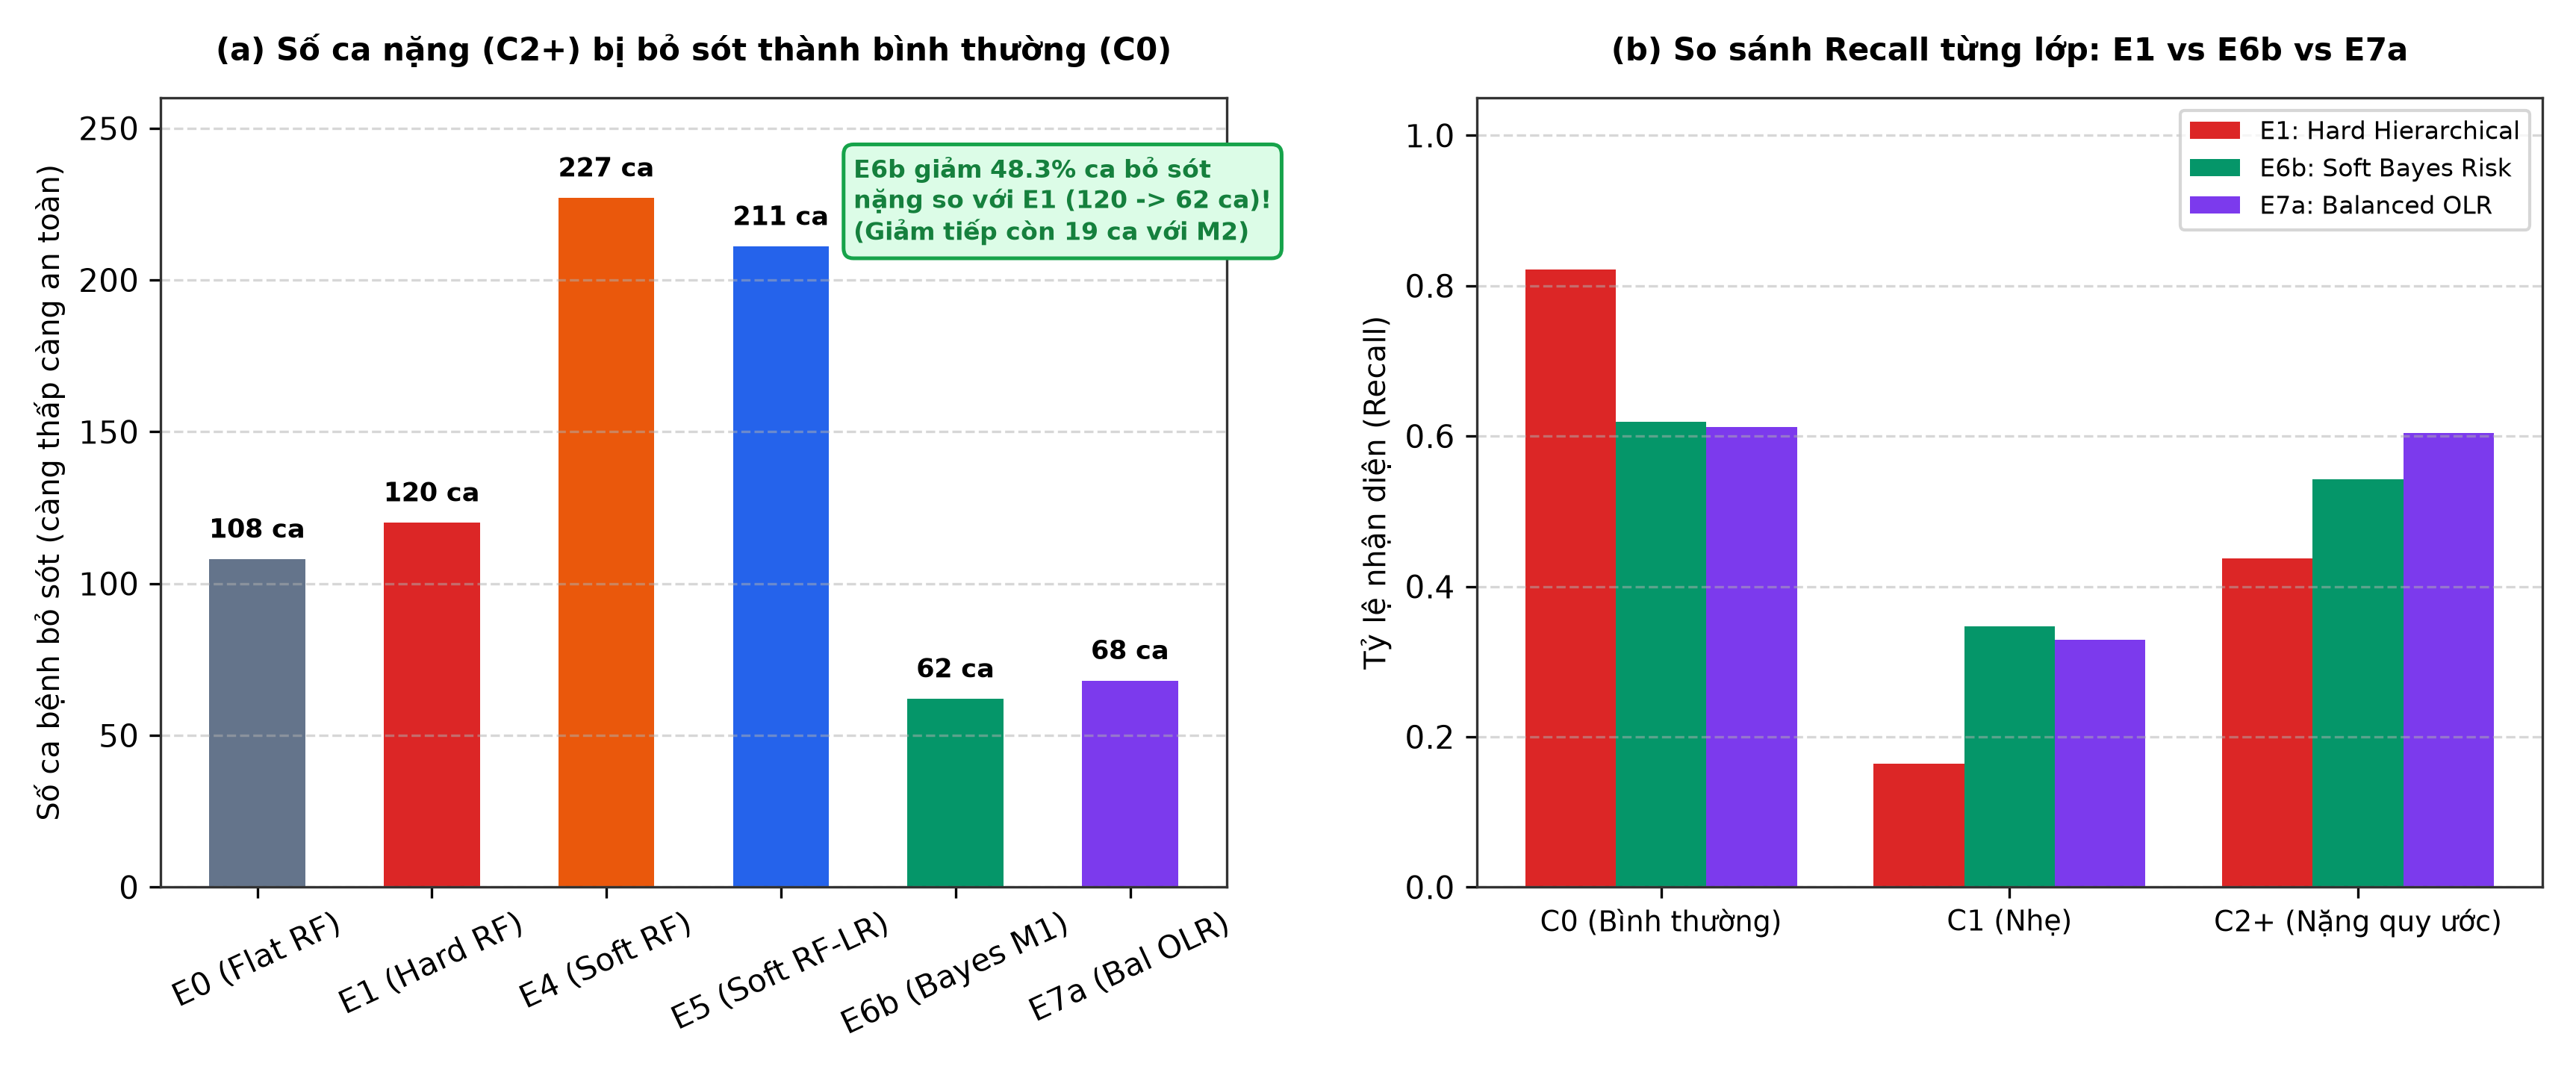
\includegraphics[width=\textwidth]{figures/fig4_confusion_error_analysis.png}
\label{fig:confusion-error-analysis}
\end{figure}
\FloatBarrier
\FloatBarrier

\subsection{Kết quả các mô hình phân loại thứ bậc ($E_7$)}
Bảng \ref{tab:ordinal-results} tổng hợp kết quả của các mô hình phân loại thứ bậc.

\begin{table}{Kết quả thực nghiệm các mô hình Ordinal Classification trên nhiệm vụ $T_3$ ($N = 4.045$)}
\centering
\footnotesize
\setlength{\tabcolsep}{3pt}
\label{tab:ordinal-results}
\begin{tabularx}{\textwidth}{l *{7}{>{\centering\arraybackslash}X}}
\toprule
\textbf{Mô hình} & \textbf{Macro-F1} & \textbf{BalAcc} & \textbf{Accuracy} & \textbf{Class MAE} & \textbf{QWK} & \textbf{Recall $C_1$} & \textbf{Recall $C_2^+$} \\
\midrule
$E_{7a}$ (OLR Unweighted) & 0.3846 & 0.4002 & \textbf{75.23\%} & \textbf{0.3377} & 0.2298 & 0.00\% & 22.00\% \\
$E_{7a}$ (OLR Balanced)   & \textbf{0.4518} & \textbf{0.5151} & 56.69\% & 0.5382 & 0.3398 & \textbf{32.93\%} & 60.37\% \\
$E_{7b}$ (CumBin LR)      & 0.3761 & 0.4949 & 63.41\% & 0.5718 & 0.2958 & 0.00\% & \textbf{72.88\%} \\
$E_{7b}$ (CumBin RF)      & 0.4191 & 0.4900 & 72.34\% & 0.3953 & \textbf{0.3744} & 0.16\% & 57.30\% \\
\bottomrule
\end{tabularx}
\end{table}


Mô hình Ordinal Logistic Regression cân bằng ($E_{7a}$ Balanced OLR) đạt \textbf{Balanced Accuracy cao nhất: 0.5151 $\pm$ 0.0152}, đồng thời nhận diện tương đối đồng đều trên cả 3 lớp: Recall $C_0 = 61.24\%$, Recall $C_1 = 32.93\%$ và Recall $C_2^+ = 60.37\%$ (Hình \ref{fig:confusion-error-analysis}b). Mặc dù Macro-F1 đạt 0.4518 (thấp hơn nhẹ so với $E_2$), sự cân bằng giữa các lớp của $E_{7a}$ tốt hơn.

Đối với mô hình Phân loại nhị phân tích lũy ($E_{7b}$ CumBin), do hai bộ phân loại $P(Y \ge 1)$ và $P(Y \ge 2)$ được huấn luyện độc lập, hiện tượng \textbf{vi phạm tính đơn điệu xác suất} $P(Y \ge 2) > P(Y \ge 1)$ xuất hiện trên thực tế (Hình \ref{fig:monotonicity-dist}): chiếm trung bình \textbf{19.53\%} tổng số dự đoán ngoài mẫu ở mô hình Logistic Regression ($E_{7b}$ CumBin LR) và \textbf{5.32\% $\pm$ 1.68\%} ở mô hình Random Forest ($E_{7b}$ CumBin RF). Sau khi áp dụng giải thuật hiệu chỉnh ngưỡng (Isotonic Probability Clipping), tỷ lệ vi phạm được đưa về 0.0\%. Tuy nhiên, việc ép xác suất $\tilde{P}(Y \ge 2) = \min(\hat{P}_1, \hat{P}_2)$ dẫn đến xác suất của lớp trung gian $P(C_1) = \hat{P}_1 - \tilde{P}_2$ bị gán bằng 0 tại các điểm vi phạm, khiến Recall của lớp $C_1$ bị suy giảm mạnh (Recall $C_1 = 0.00\%$ ở LR và $0.16\%$ ở RF).

\begin{figure}[htbp]{Phân bố vi phạm tính đơn điệu xác suất trong mô hình phân loại nhị phân tích lũy $E_{7b}$}
\centering
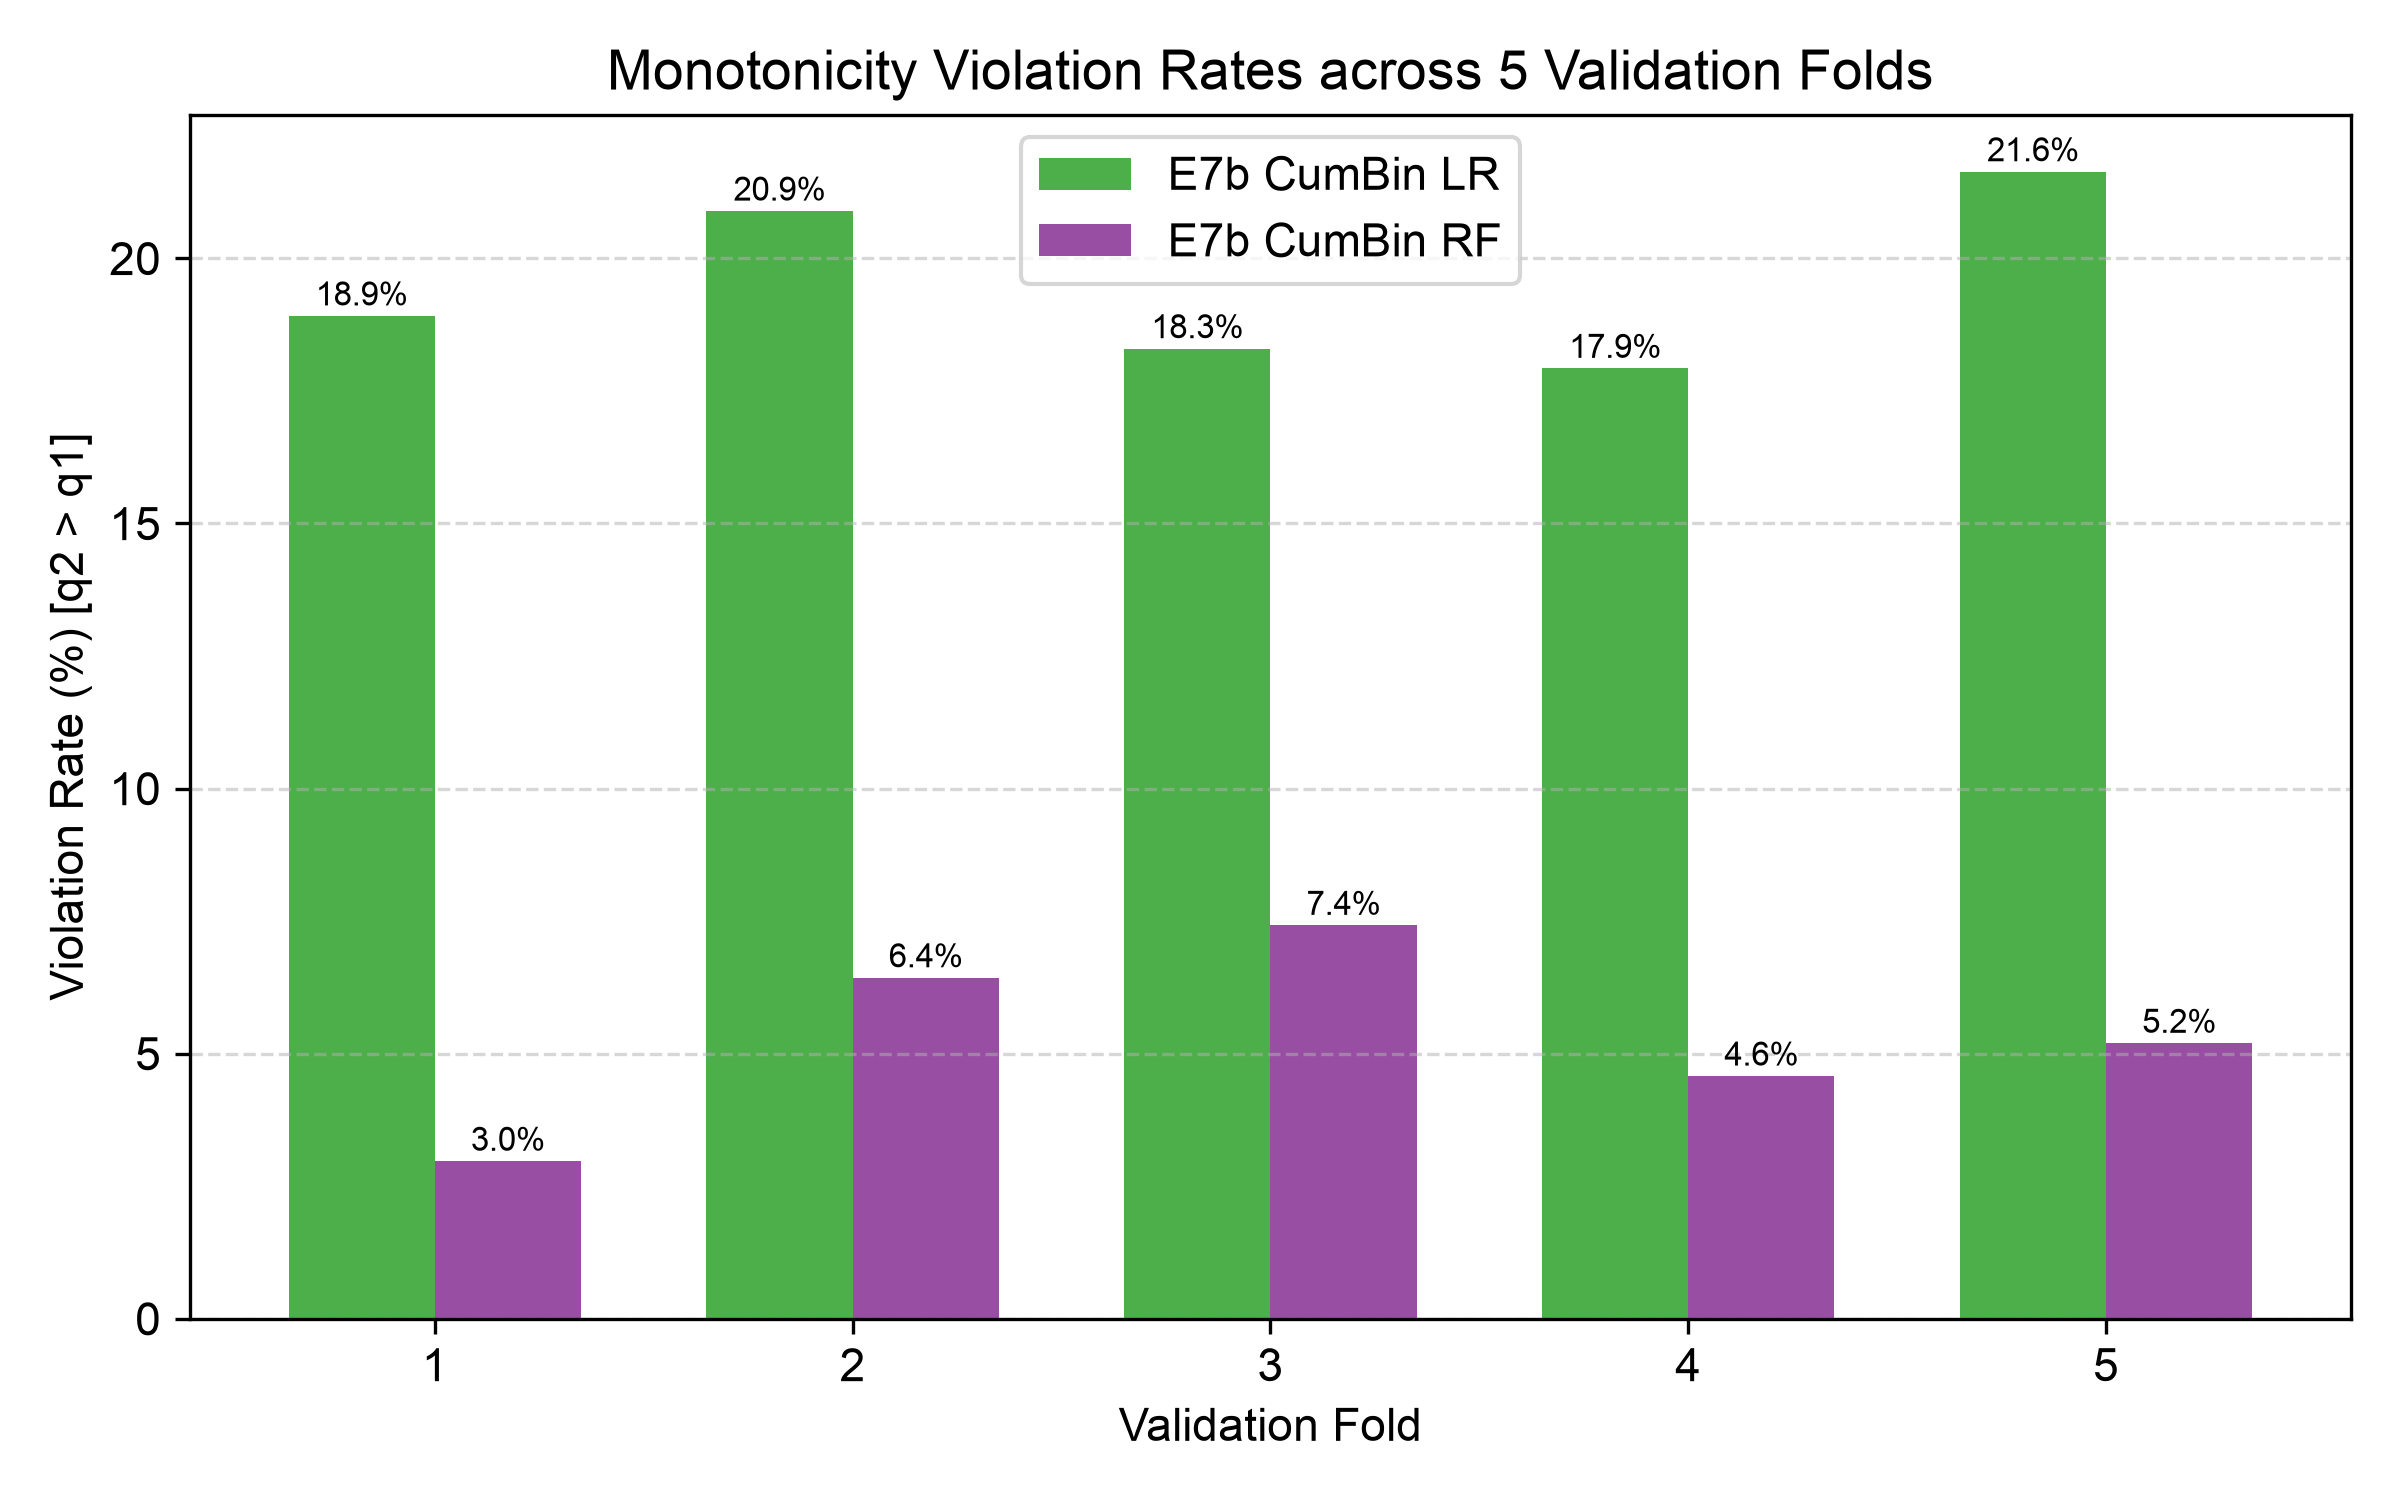
\includegraphics[width=0.8\textwidth]{figures/monotonicity_violation_distribution.png}
\label{fig:monotonicity-dist}
\end{figure}
\FloatBarrier

\subsection{Bảng so sánh tổng hợp các mô hình $T_3$}
Bảng \ref{tab:master-comparison} tổng hợp so sánh các mô hình từ $E_0$ đến $E_7$ trên hai nhóm chỉ số: hiệu năng phân loại tổng thể (Phần A) và các chỉ số liên quan đến sai số sàng lọc (Phần B).

\begin{table}{So sánh kết quả các mô hình trên nhiệm vụ $T_3$ ($N = 4.045$)}
\centering
\footnotesize
\setlength{\tabcolsep}{4pt}
\label{tab:master-comparison}

\vspace{-0.1cm}
\textbf{Phần A: Tổng hợp các chỉ số hiệu năng phân loại tổng thể}
\vspace{0.15cm}

\begin{tabularx}{\textwidth}{l X c c c c c}
\toprule
\textbf{Nhóm mô hình} & \textbf{Mô hình} & \textbf{Macro-F1} & \textbf{BalAcc} & \textbf{Accuracy} & \textbf{Class MAE} & \textbf{QWK} \\
\midrule
\textbf{Flat} & $E_0$ (Flat RF) & 0.4354 & 0.4667 & 64.10\% & 0.4638 & 0.3204 \\
\midrule
\multirow{4}{*}{\textbf{Hard Hier.}} 
  & $E_1$ (Hard RF--RF)   & 0.4550 & 0.4745 & 68.08\% & 0.4133 & 0.3705 \\
  & $E_2$ (Hard Tuned)    & \textbf{0.4586} & 0.4745 & 65.32\% & 0.4280 & 0.3644 \\
  & $E_{3a}$ (Hard RF--LR) & 0.4567 & 0.4964 & 68.43\% & 0.4195 & 0.3735 \\
  & $E_{3b}$ (Hard RF--XGB)& 0.4575 & 0.4790 & 68.23\% & 0.4180 & 0.3683 \\
\midrule
\multirow{2}{*}{\textbf{Soft Hier.}} 
  & $E_4$ (Soft RF--RF Argmax) & 0.4206 & 0.4309 & 73.75\% & 0.3530 & 0.3653 \\
  & $E_5$ (Soft RF--LR Argmax) & 0.4270 & 0.4506 & 73.37\% & 0.3619 & 0.3789 \\
\midrule
\multirow{2}{*}{\textbf{Cost-Sens.}}
  & $E_{6a}$ (Soft Cost RF--RF $M_1$) & 0.4535 & 0.4904 & 56.91\% & 0.5216 & 0.3235 \\
  & $E_{6b}$ (Soft Cost RF--LR $M_1$) & 0.4521 & 0.5025 & 56.84\% & 0.5197 & 0.3344 \\
\midrule
\multirow{4}{*}{\textbf{Ordinal}} 
  & $E_{7a}$ (OLR Unweighted) & 0.3846 & 0.4002 & \textbf{75.23\%} & \textbf{0.3377} & 0.2298 \\
  & $E_{7a}$ (OLR Balanced)   & 0.4518 & \textbf{0.5151} & 56.69\% & 0.5382 & 0.3398 \\
  & $E_{7b}$ (CumBin LR)      & 0.3761 & 0.4949 & 63.41\% & 0.5718 & 0.2958 \\
  & $E_{7b}$ (CumBin RF)      & 0.4191 & 0.4900 & 72.34\% & 0.3953 & \textbf{0.3744} \\
\midrule
\textbf{Baseline} & Majority Class ($C_0$) & 0.2848 & 0.3333 & 74.56\% & 0.3518 & 0.0000 \\
\bottomrule
\end{tabularx}

\vspace{0.35cm}
\textbf{Phần B: Khả năng nhận diện từng lớp và chỉ số sai số sàng lọc}
\vspace{0.15cm}

\begin{tabularx}{\textwidth}{l X c c c c c}
\toprule
\textbf{Nhóm mô hình} & \textbf{Mô hình} & \textbf{Recall $C_0$} & \textbf{Recall $C_1$} & \textbf{Recall $C_2^+$} & \textbf{$C_2^+ \to C_0$} & \textbf{$C_0 \to C_2^+$} \\
\midrule
\textbf{Flat} & $E_0$ (Flat RF) & 76.39\% & 16.29\% & 47.32\% & 108 ca & 316 ca \\
\midrule
\multirow{4}{*}{\textbf{Hard Hier.}} 
  & $E_1$ (Hard RF--RF)   & 82.16\% & 16.46\% & 43.74\% & 120 ca & 261 ca \\
  & $E_2$ (Hard Tuned)    & 77.02\% & 25.69\% & 39.63\% & 98 ca & 222 ca \\
  & $E_{3a}$ (Hard RF--LR) & 82.16\% & 11.75\% & 55.00\% & 120 ca & 300 ca \\
  & $E_{3b}$ (Hard RF--XGB)& 82.16\% & 16.77\% & 44.76\% & 120 ca & 279 ca \\
\midrule
\multirow{2}{*}{\textbf{Soft Hier.}} 
  & $E_4$ (Soft RF--RF Argmax) & 93.90\% & 5.18\% & 30.19\% & 227 ca & 139 ca \\
  & $E_5$ (Soft RF--LR Argmax) & 92.61\% & 3.45\% & 39.13\% & 211 ca & 176 ca \\
\midrule
\multirow{2}{*}{\textbf{Cost-Sens.}}
  & $E_{6a}$ (Soft Cost RF--RF $M_1$) & 61.94\% & \textbf{40.92\%} & 44.25\% & \textbf{62 ca} & 215 ca \\
  & $E_{6b}$ (Soft Cost RF--LR $M_1$) & 61.87\% & 34.64\% & 54.23\% & \textbf{62 ca} & 294 ca \\
\midrule
\multirow{4}{*}{\textbf{Ordinal}} 
  & $E_{7a}$ (OLR Unweighted) & 98.04\% & 0.00\% & 22.00\% & 305 ca & \textbf{59 ca} \\
  & $E_{7a}$ (OLR Balanced)   & 61.24\% & 32.93\% & 60.37\% & 68 ca & 357 ca \\
  & $E_{7b}$ (CumBin LR)      & 75.60\% & 0.00\% & \textbf{72.88\%} & 106 ca & 727 ca \\
  & $E_{7b}$ (CumBin RF)      & 89.56\% & 0.16\% & 57.30\% & 167 ca & 313 ca \\
\midrule
\textbf{Baseline} & Majority Class ($C_0$) & \textbf{100.00\%} & 0.00\% & 0.00\% & 391 ca & 0 ca \\
\bottomrule
\end{tabularx}

\vspace{0.15cm}
\raggedright
\scriptsize
\textit{Ghi chú:} Các giá trị Recall là trung bình cộng qua 5 fold kiểm định chéo ngoài mẫu (đồng thời khớp tuyệt đối với tỷ lệ trên ma trận nhầm lẫn gộp pooled out-of-fold, độ lệch $< 0.02\%$). Số ca phân loại sai ($C_2^+ \to C_0$ và $C_0 \to C_2^+$) là số lượng tuyệt đối tổng hợp từ toàn bộ dự đoán ngoài mẫu (pooled OOF, $N = 4.045$).
\end{table}


Hình \ref{fig:legacy-comparison} trực quan hóa sự so sánh giữa các mô hình từ $E_0$ đến $E_6$. Hình \ref{fig:macro-vs-mae} và Hình \ref{fig:2step-errors} phân tích mối quan hệ giữa Macro-F1, Class MAE và tỷ lệ lỗi nhảy 2 bước ($C_2^+ \to C_0$).

\begin{figure}[htbp]{So sánh trực quan hiệu năng giữa các mô hình từ $E_0$ đến $E_6$ trên tập Legacy}
\centering
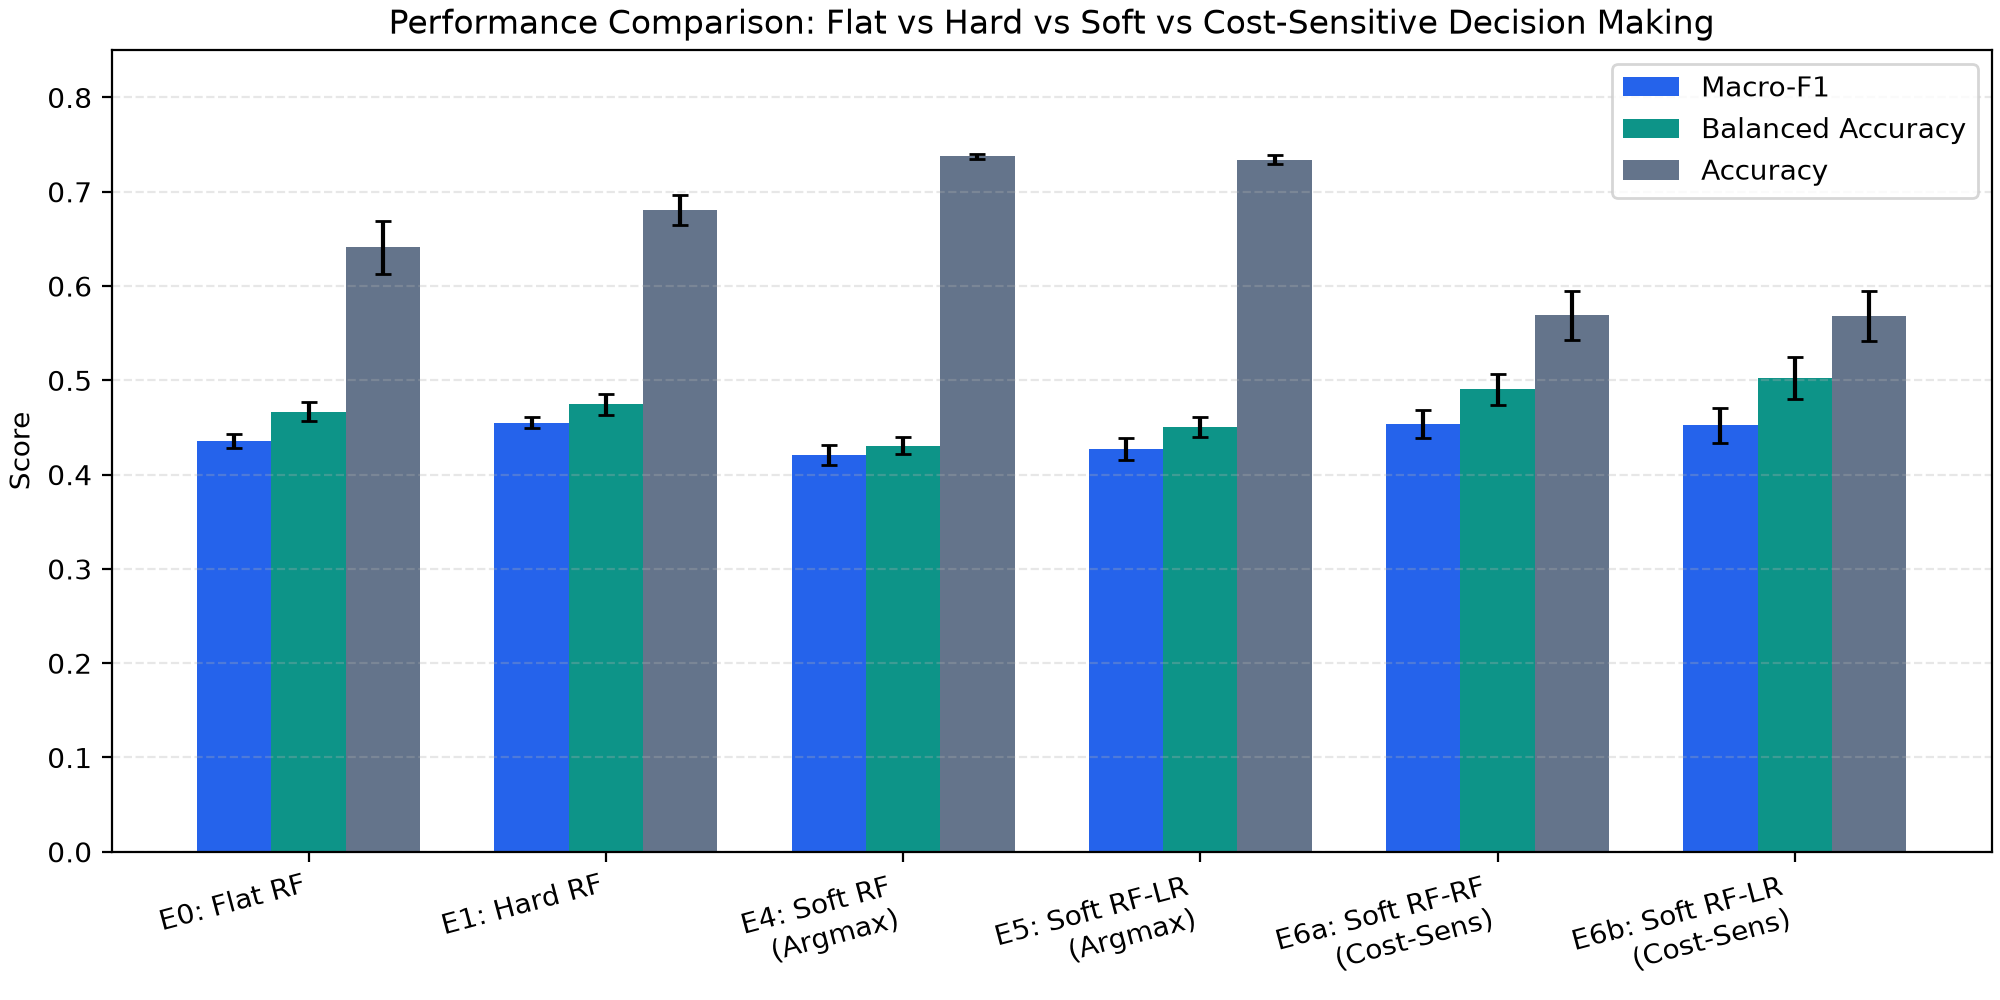
\includegraphics[width=0.85\textwidth]{figures/legacy_model_comparison_e0_to_e6.png}
\label{fig:legacy-comparison}
\end{figure}
\FloatBarrier

\begin{figure}[htbp]{Mối quan hệ đánh đổi giữa Macro-F1 và Class MAE giữa các hướng tiếp cận mô hình}
\centering
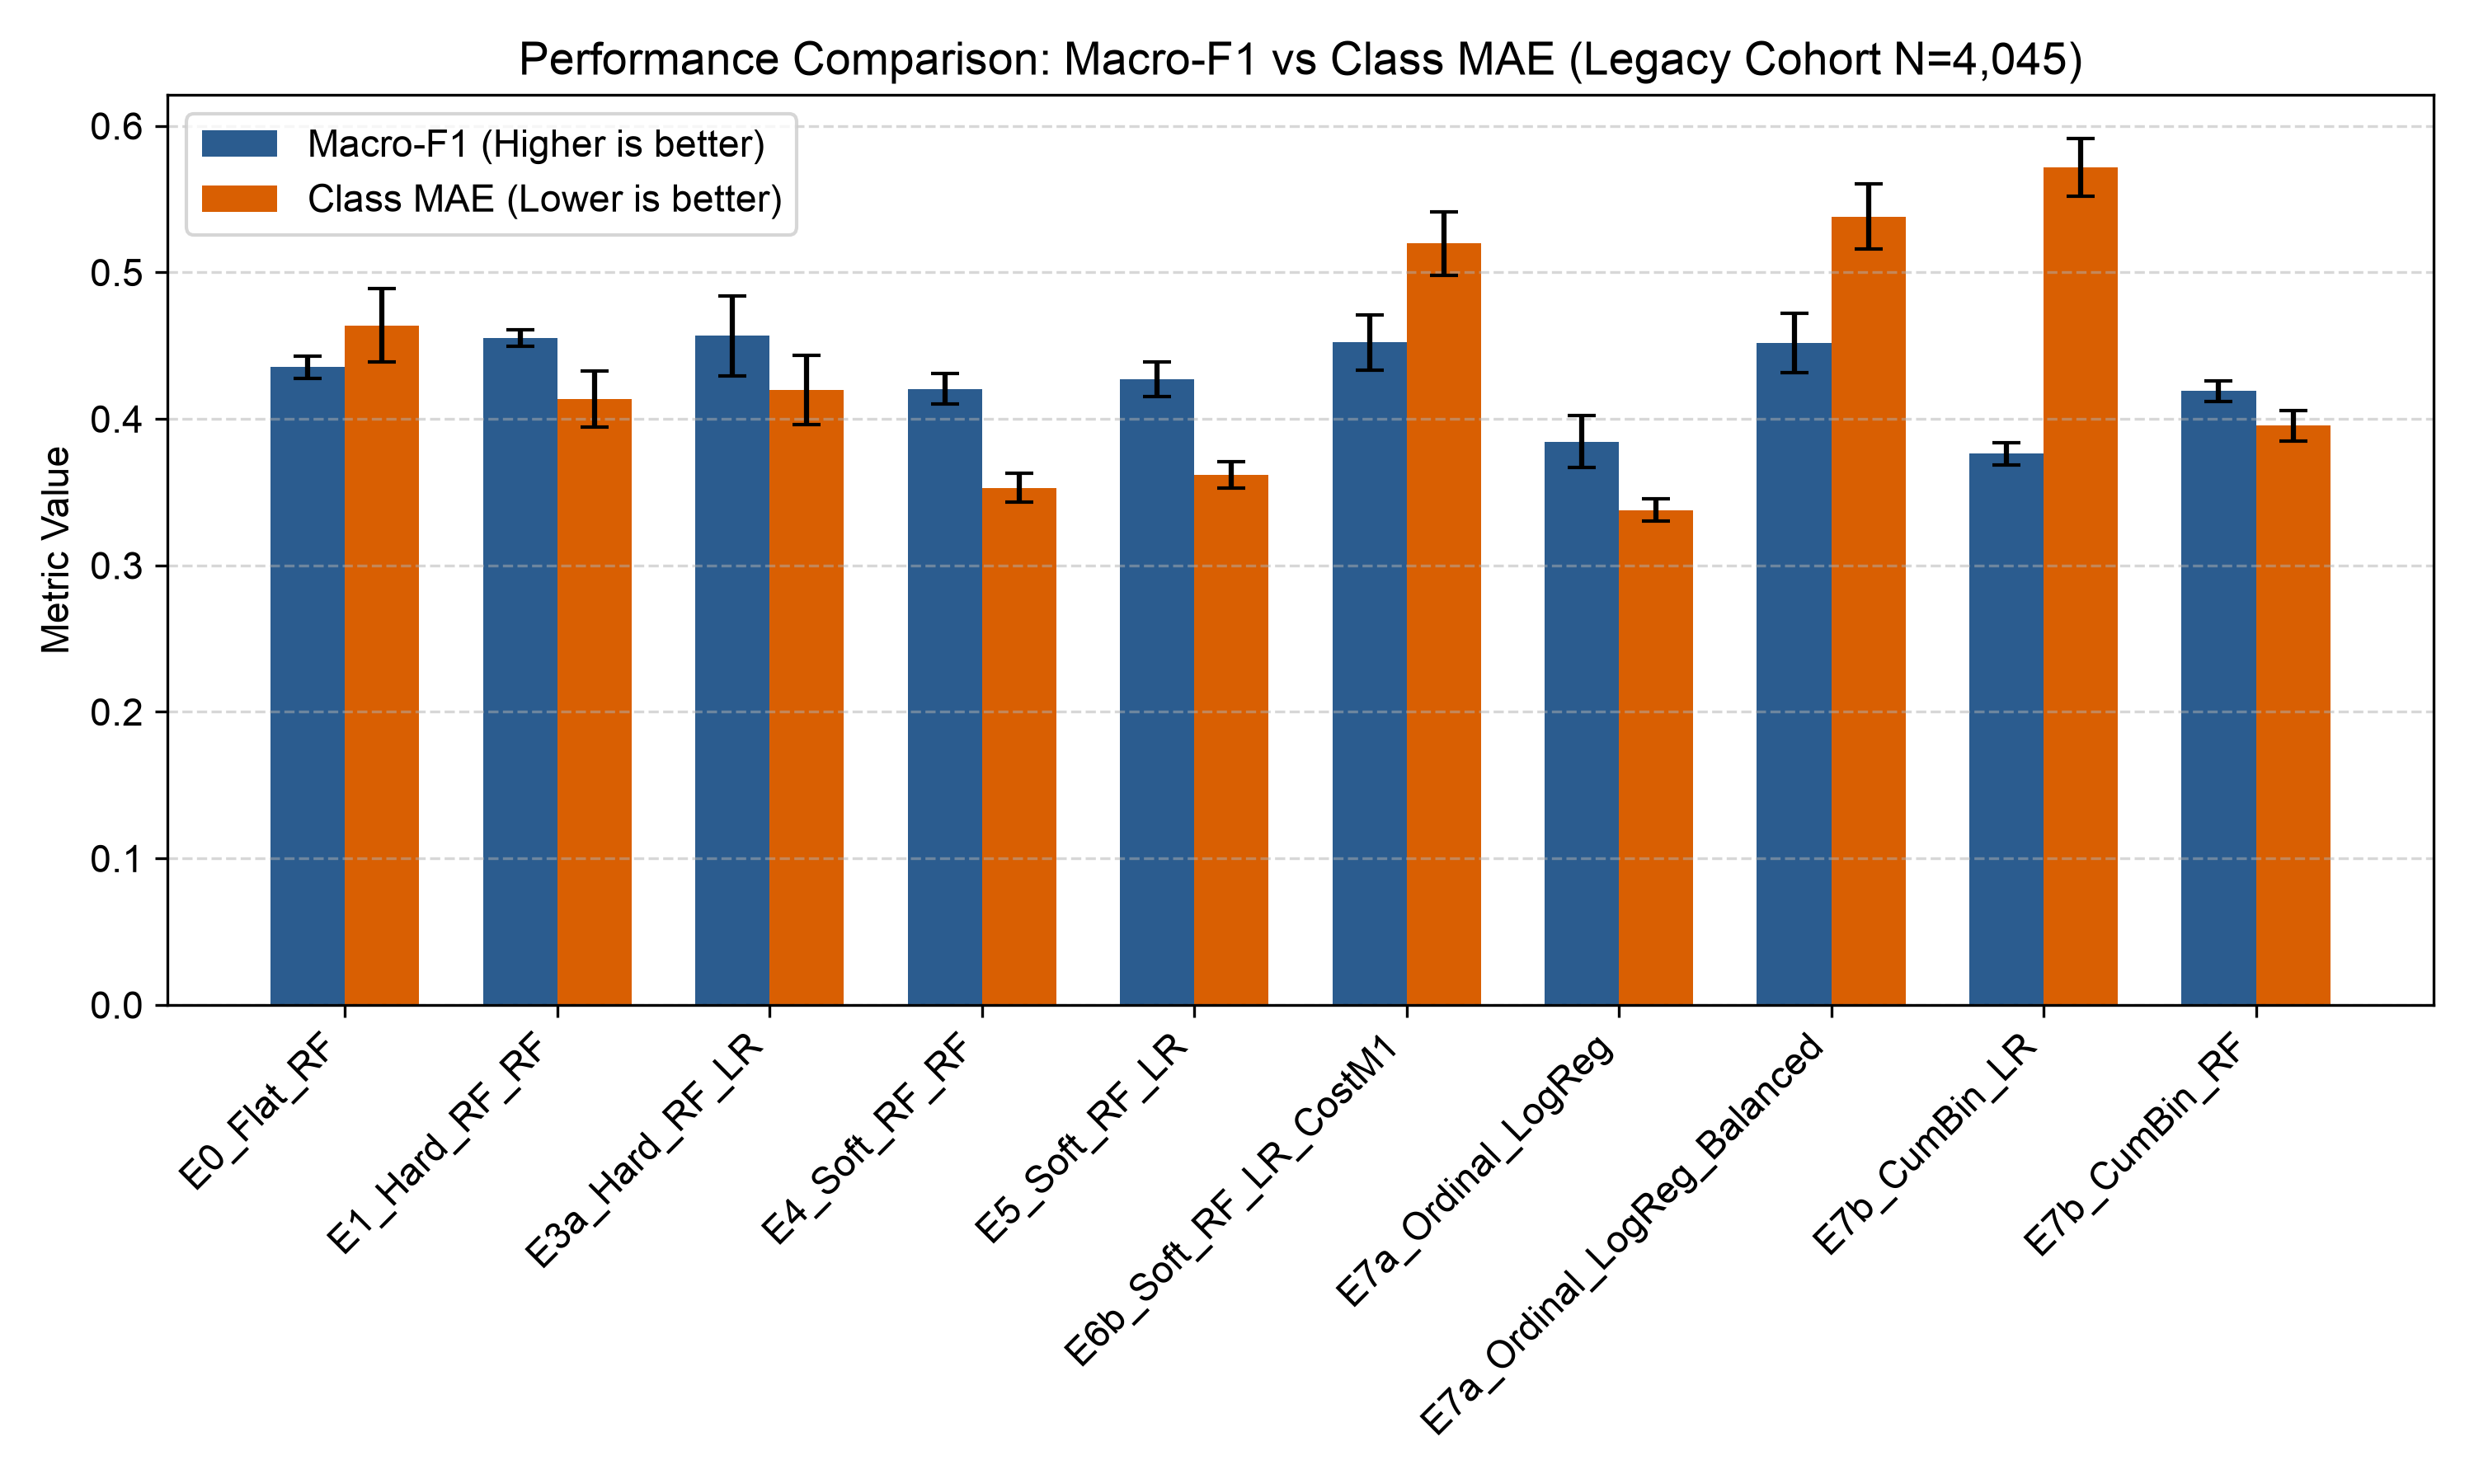
\includegraphics[width=0.85\textwidth]{figures/macro_f1_vs_mae.png}
\label{fig:macro-vs-mae}
\end{figure}
\FloatBarrier

\begin{figure}[htbp]{So sánh số lượng lỗi nhảy 2 bước ($C_2^+ \to C_0$) giữa các mô hình}
\centering
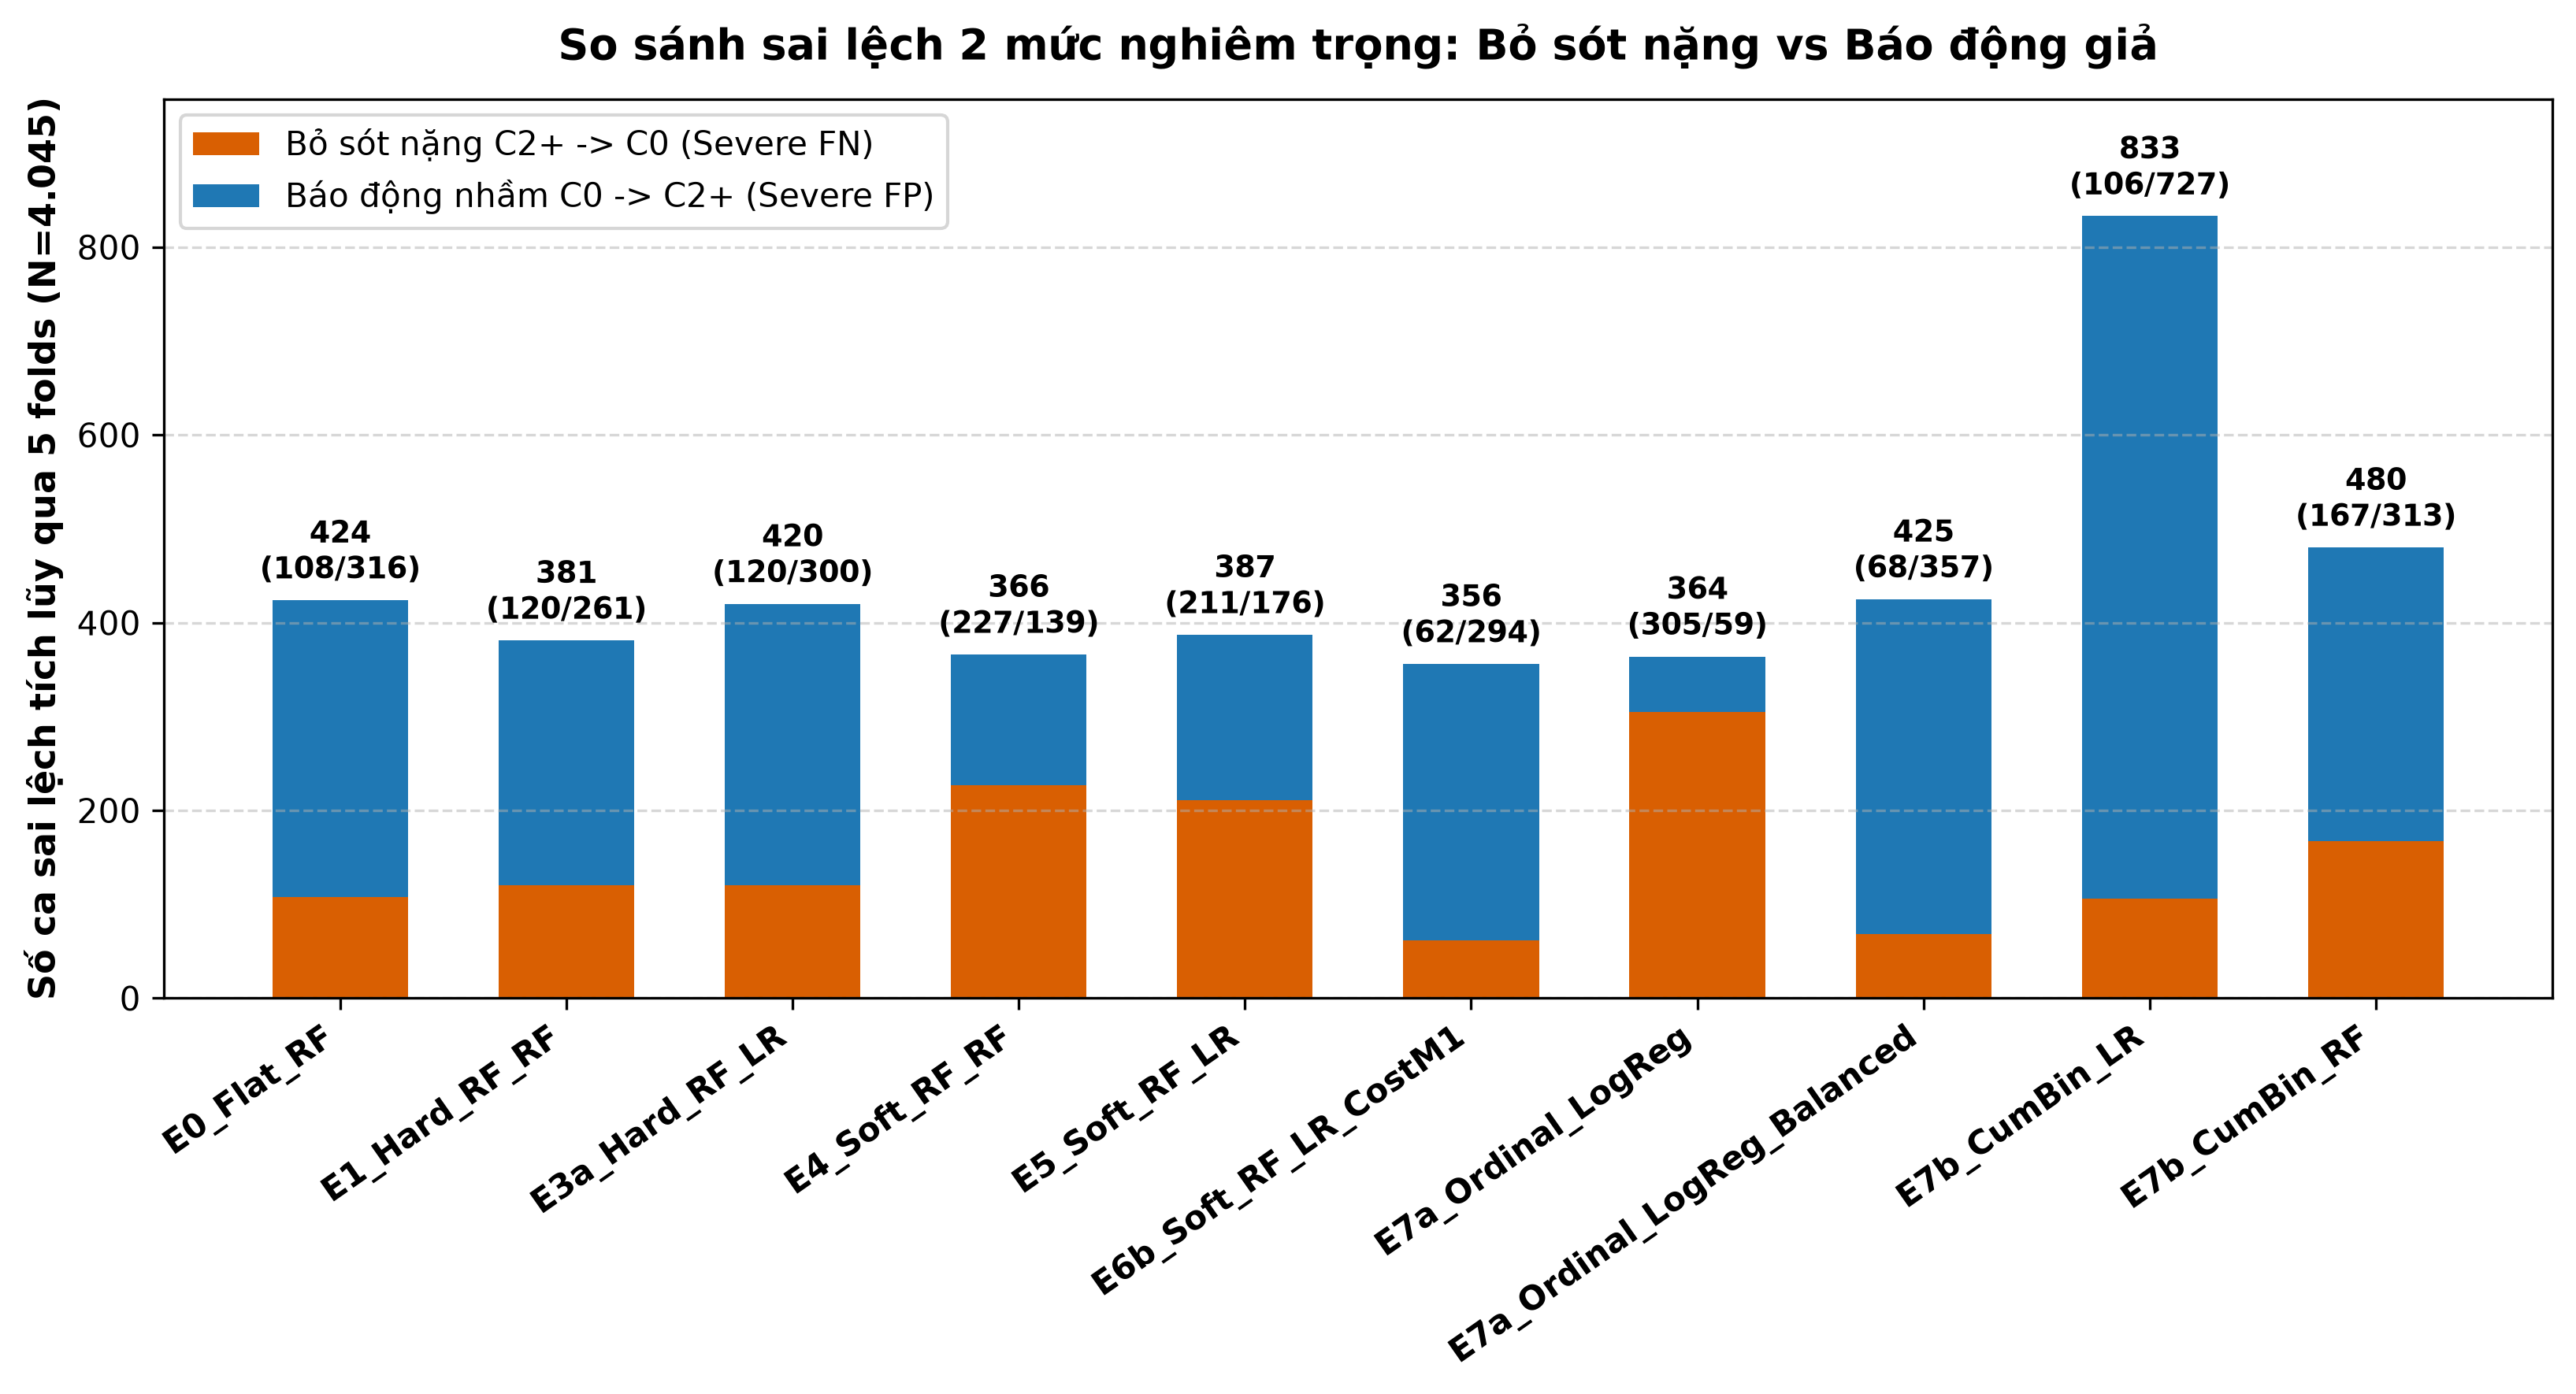
\includegraphics[width=0.85\textwidth]{figures/2step_error_comparison.png}
\label{fig:2step-errors}
\end{figure}
\FloatBarrier

Hình \ref{fig:conf-p1} và Hình \ref{fig:conf-p2} trình bày ma trận nhầm lẫn chi tiết của 6 mô hình đại diện: $E_0, E_1, E_5, E_{6b}, E_{7a}, E_{7b}$.

\begin{figure}[htbp]{Ma trận nhầm lẫn của 4 mô hình đại diện: $E_0$ (Flat RF), $E_1$ (Hard RF--RF), $E_5$ (Soft RF--LR) và $E_{6b}$ (Cost-Sensitive)}
\centering
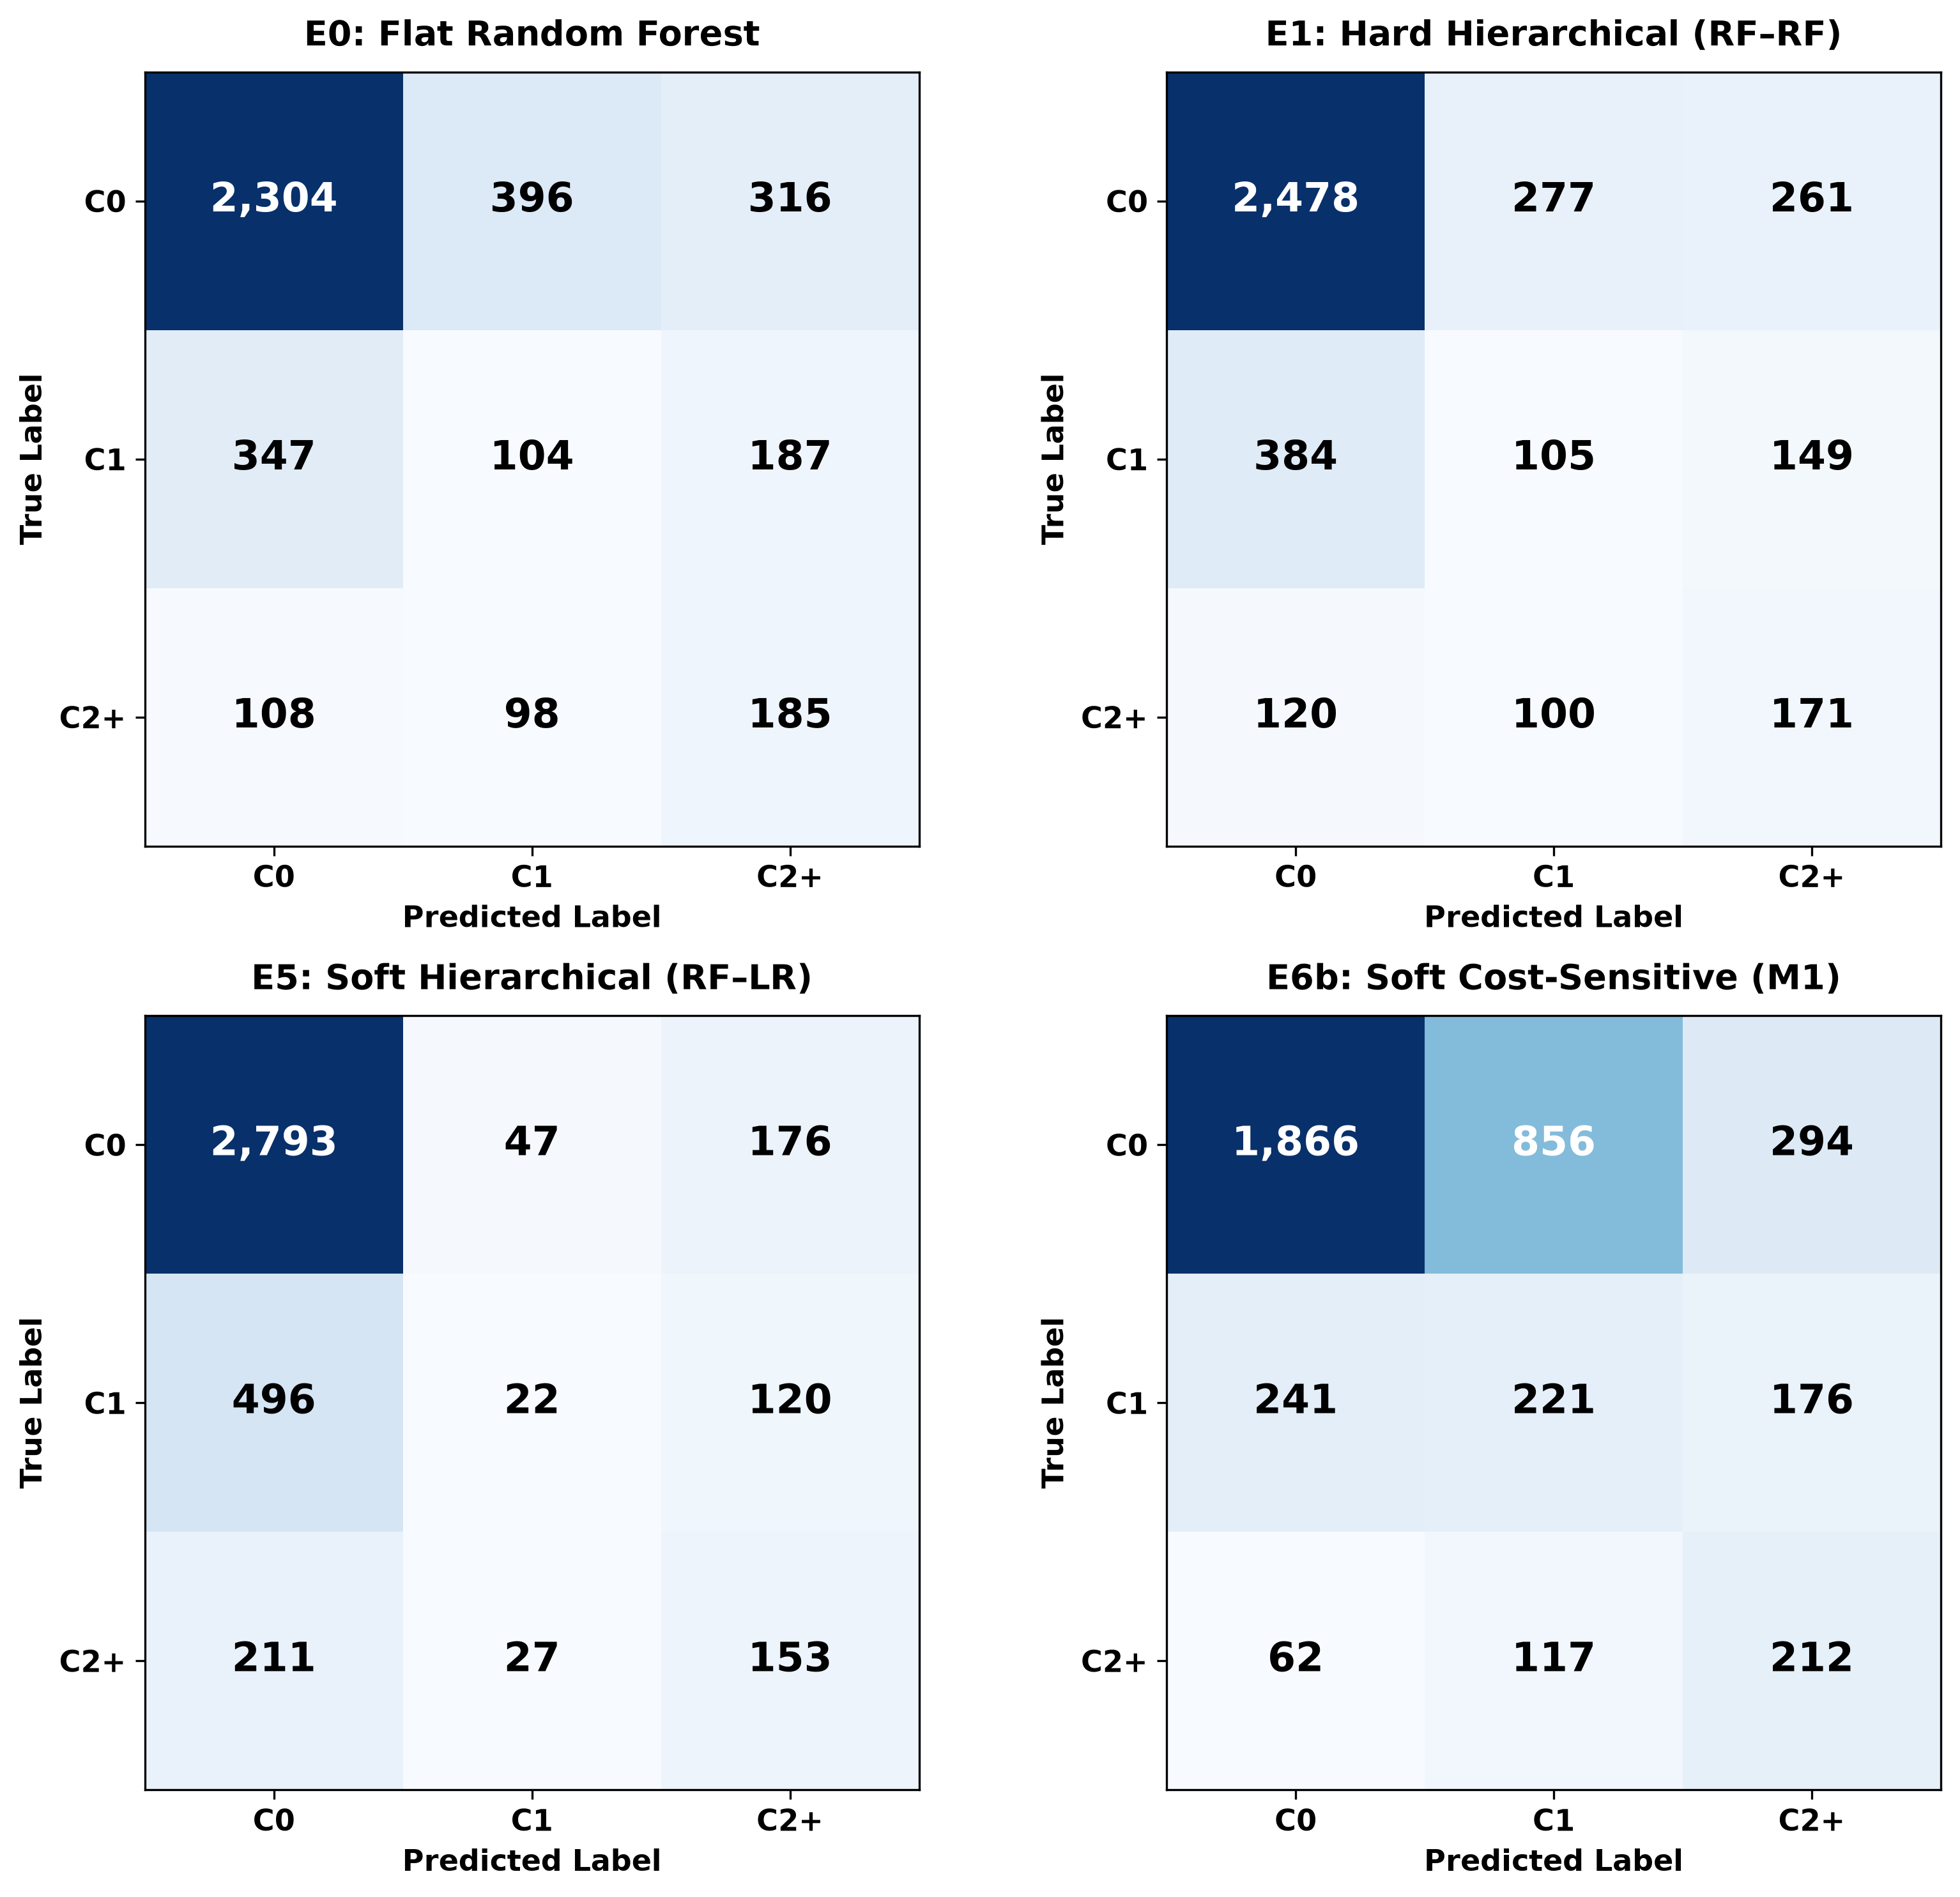
\includegraphics[width=0.95\textwidth]{figures/confusion_matrices_group1.png}
\label{fig:conf-p1}
\end{figure}
\FloatBarrier

\begin{figure}[htbp]{Ma trận nhầm lẫn của 2 mô hình phân loại thứ bậc: $E_{7a}$ (Balanced OLR) và $E_{7b}$ (CumBin RF)}
\centering
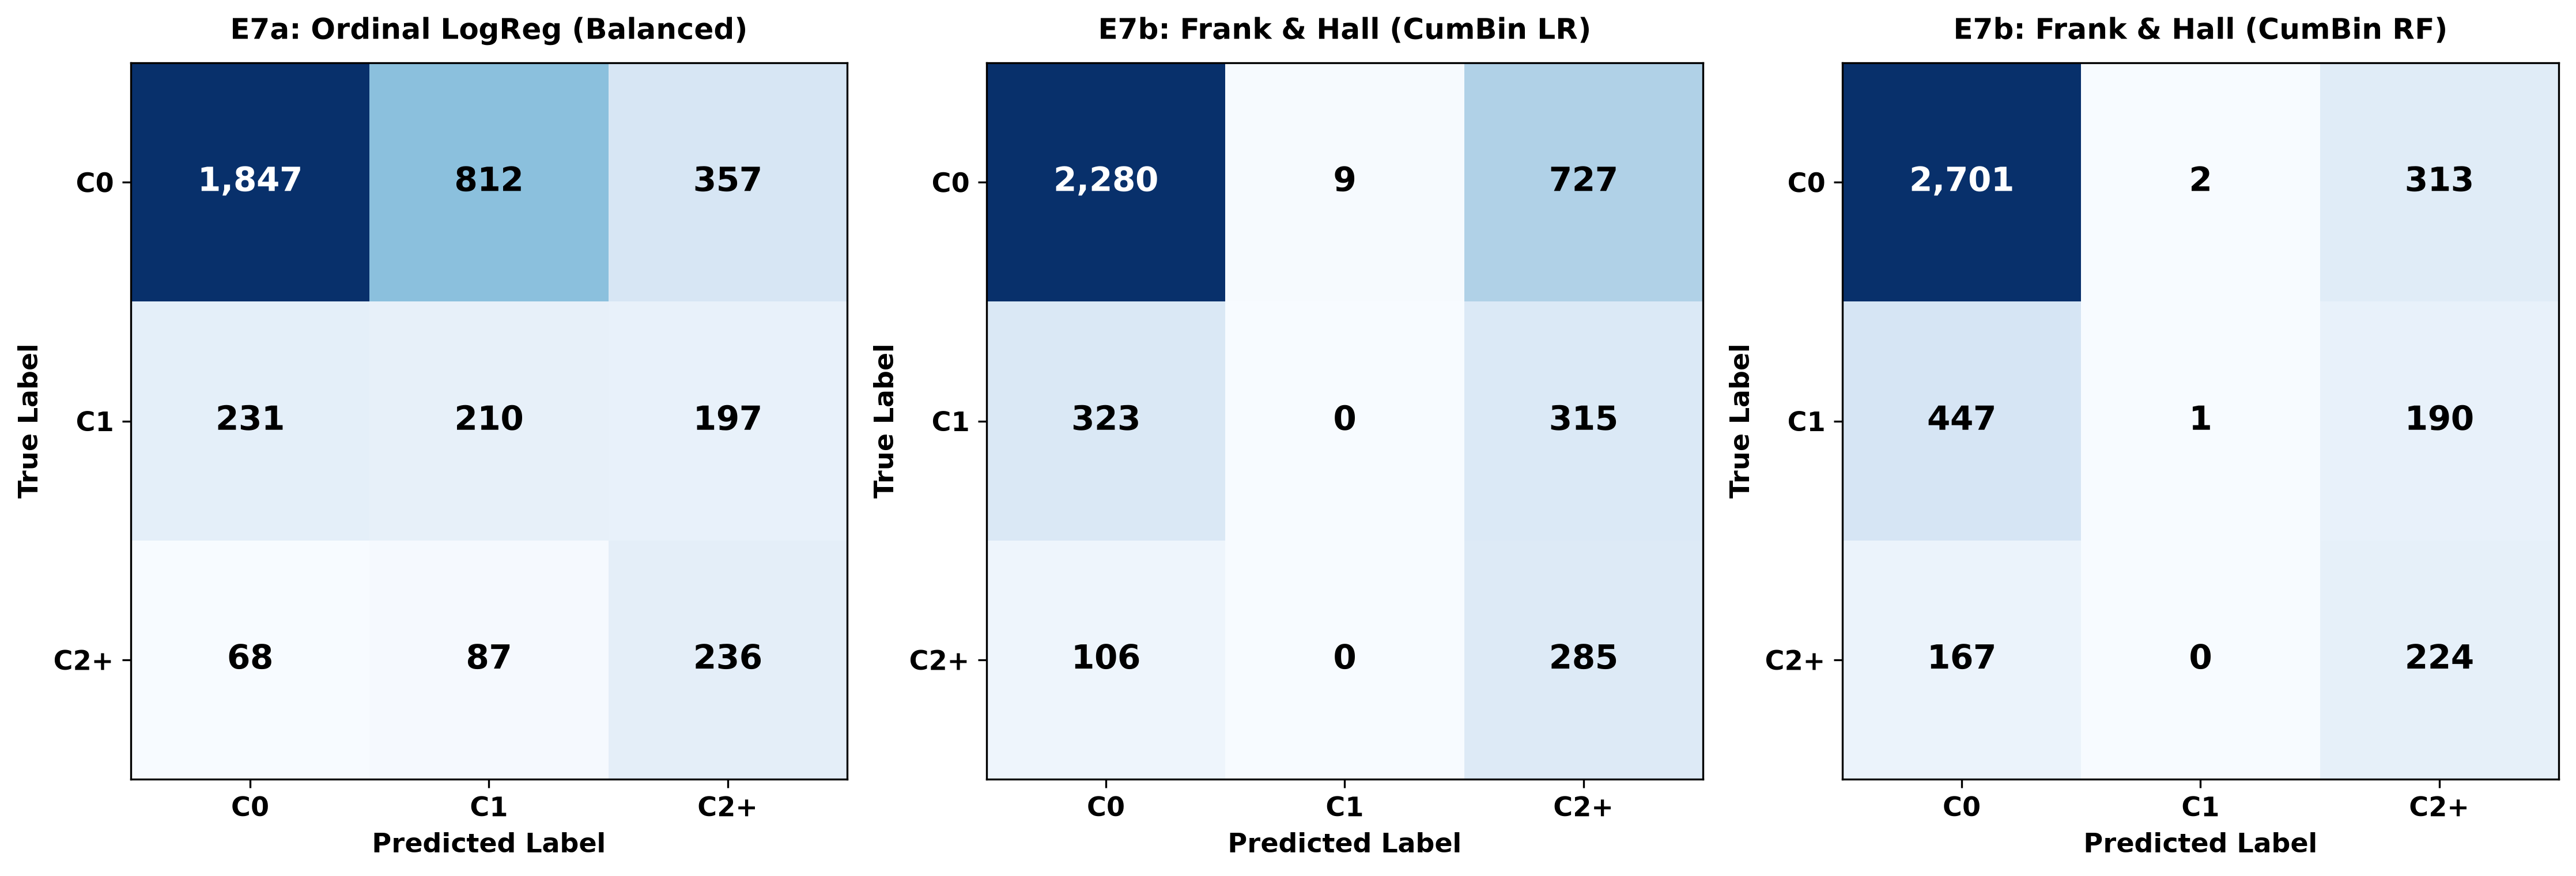
\includegraphics[width=0.95\textwidth]{figures/confusion_matrices_group2.png}
\label{fig:conf-p2}
\end{figure}
\FloatBarrier

\section{Phân tích sự đánh đổi sai số và ma trận chi phí}
\label{sec:danh-doi-lam-sang}

Một kết quả thực nghiệm quan trọng của DepSev-ML là định lượng sự đánh đổi giữa hai loại sai số (Hình \ref{fig:cost-tradeoff}):
\begin{itemize}
    \item \textbf{Sai số bỏ sót ca nặng ($C_2^+ \to C_0$):} Nguy cơ bỏ sót đối tượng có triệu chứng nặng trong quá trình sàng lọc.
    \item \textbf{Sai số báo động nhầm ($C_0 \to C_2^+$):} Khiến đối tượng có triệu chứng tối thiểu bị phân loại nhầm vào nhóm nặng, làm tăng chi phí theo dõi không cần thiết.
\end{itemize}

\begin{figure}[htbp]{Đường cong đánh đổi giữa tỷ lệ nhận diện ca nặng ($C_2^+$ Recall) và tỷ lệ báo động nhầm ($C_0$ False Alarm Rate)}
\centering
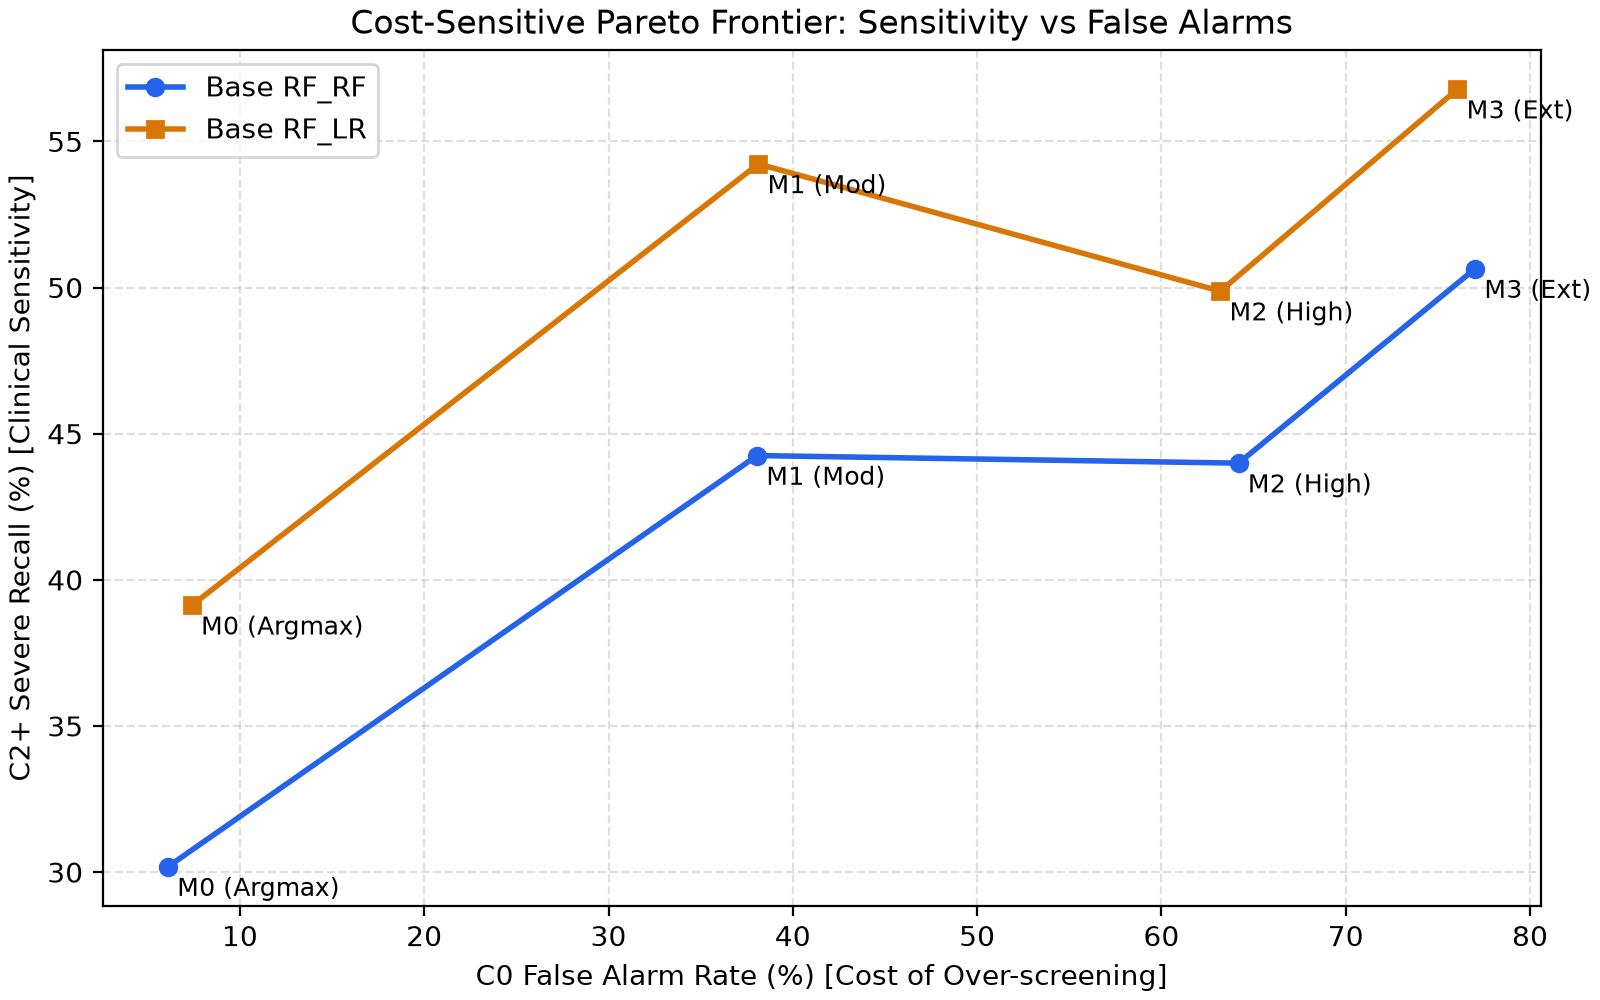
\includegraphics[width=0.85\textwidth]{figures/cost_tradeoff_curve.png}
\label{fig:cost-tradeoff}
\end{figure}
\FloatBarrier

Khi điều chỉnh mức độ phạt từ ma trận $M_0$ (chi phí đồng nhất) đến $M_3$ (phạt tối đa lỗi bỏ sót ca nặng $\mathbf{C}(2, 0) = 8.0$):
\begin{itemize}
    \item Số ca nặng bị bỏ sót thành bình thường ($C_2^+ \to C_0$) giảm từ \textbf{120 ca ($E_1$)} xuống còn \textbf{62 ca ($E_{6b}$, ma trận $M_1$)}, tương đương mức giảm \textbf{48.33\%} (tỷ lệ bỏ sót giảm từ 30.69\% xuống 15.86\%). Khi tăng cường mức phạt sang $M_2$ ($\mathbf{C}(2, 0) = 5.0$) và $M_3$ ($\mathbf{C}(2, 0) = 8.0$), số ca bỏ sót tiếp tục giảm xuống lần lượt \textbf{19 ca} (giảm 84.17\%) và \textbf{7 ca} (giảm 94.17\%). (Lưu ý: ở cấu hình phân cấp mềm $E_5$ sử dụng hàm argmax thuần túy, do xu hướng thiên lệch về lớp đa số $C_0$, số ca bỏ sót là 211 ca).
    \item Đổi lại, số ca bình thường bị xếp sang nhóm có triệu chứng ($C_0 \to \{C_1, C_2^+\}$) tăng từ 538 ca ($E_1$) lên \textbf{1.150 ca ($E_{6b}$, $M_1$)} (trong đó 294 ca bị xếp trực tiếp thành $C_2^+$), và tiếp tục tăng lên 1.906 ca ($M_2$) cùng 2.294 ca ($M_3$).
\end{itemize}
Đây là quy luật đánh đổi tự nhiên trong sàng lọc sức khỏe cộng đồng. Khung làm việc DepSev-ML cho phép lựa chọn ma trận chi phí phù hợp tùy thuộc vào năng lực tiếp nhận của hệ thống y tế thực tế.

\section{Kiểm định ngoại suy theo dòng thời gian (Temporal Validation)}
\label{sec:temporal-results}

Để kiểm tra xem liệu các kết quả trên có bị quá khớp trên một chu kỳ khảo sát đơn lẻ hay không, nghiên cứu thực hiện kiểm định ngoại suy trên tập dữ liệu độc lập NHANES 2015--2016 ($N = 4.888$, Branch D). Toàn bộ các mô hình được huấn luyện trên dữ liệu gộp hai chu kỳ 2011--2014 ($N = 9.693$) và kiểm định ngoại suy một lần duy nhất trên chu kỳ 2015--2016 ($N = 4.888$), áp dụng trên không gian 31 đặc trưng hài hòa hóa ($F_{4\_\text{common31}}$).

Kết quả được trình bày trong Bảng \ref{tab:multicycle-temporal-results}. Hình \ref{fig:multicycle-soft-temporal} minh họa sự so sánh hiệu năng của các mô hình phân cấp mềm và nhạy chi phí qua ba nhánh dữ liệu (Branch A, B, D).

\begin{table}{Kết quả kiểm định ngoại suy theo dòng thời gian (Branch D, NHANES 2015--2016, $N = 4.888$)}
\centering
\footnotesize
\setlength{\tabcolsep}{3pt}
\label{tab:multicycle-temporal-results}
\begin{tabularx}{\textwidth}{l *{7}{>{\centering\arraybackslash}X}}
\toprule
\textbf{Mô hình ($T_3$)} & \textbf{Macro-F1} & \textbf{BalAcc} & \textbf{Accuracy} & \textbf{Recall $C_0$} & \textbf{Recall $C_1$} & \textbf{Recall $C_2^+$} & \textbf{Class MAE} \\
\midrule
$E_0$ (Flat RF)                     & 0.4345 & 0.4908 & 62.68\% & 73.66\% & 18.79\% & 54.77\% & 0.5008 \\
$E_1$ (Hard RF--RF)                 & \textbf{0.4393} & 0.4879 & 66.35\% & 79.86\% & 14.51\% & 52.01\% & 0.4556 \\
$E_4$ (Soft RF--RF)                 & 0.4223 & 0.4594 & \textbf{71.91\%} & 90.60\% & 4.76\% & 42.46\% & \textbf{0.3766} \\
$E_5$ (Soft RF--LR)                 & 0.4265 & 0.4681 & 71.79\% & 90.08\% & 4.88\% & 45.48\% & 0.3801 \\
$E_{6b}$ (Soft Cost $M_2$)          & 0.3439 & 0.4691 & 34.84\% & 26.94\% & \textbf{60.29\%} & 53.52\% & 0.7306 \\
$E_{7a}$ (OLR Balanced)             & 0.4349 & \textbf{0.5073} & 56.28\% & 61.74\% & 31.15\% & 59.30\% & 0.5503 \\
$E_{7b}$ (CumBin LR)                & 0.3632 & 0.4982 & 62.21\% & 75.23\% & 0.12\% & \textbf{74.12\%} & 0.5833 \\
$E_{7b}$ (CumBin RF)                & 0.3861 & 0.4861 & 67.88\% & 84.16\% & 0.36\% & 61.31\% & 0.4695 \\
\bottomrule
\end{tabularx}

\vspace{0.15cm}
\raggedright
\scriptsize
\textit{Ghi chú:} Mô hình được huấn luyện trên dữ liệu 2 chu kỳ 2011--2014 ($N = 9.693$) và kiểm tra ngoại suy độc lập một lần duy nhất trên chu kỳ 2015--2016 ($N = 4.888$) với không gian 31 đặc trưng hài hòa ($F_{4\_\text{common31}}$). Cấu hình $E_{6b}$ ở đây áp dụng ma trận chi phí phạt nặng $M_2$, dẫn đến Recall $C_0$ giảm còn 26.94\% để ưu tiên độ nhạy cho các nhóm có triệu chứng.
\end{table}


\begin{figure}[htbp]{So sánh hiệu năng các mô hình phân cấp mềm và nhạy chi phí giữa chu kỳ đơn lẻ (Branch A), gộp đa chu kỳ (Branch B) và kiểm định thời gian (Branch D)}
\centering
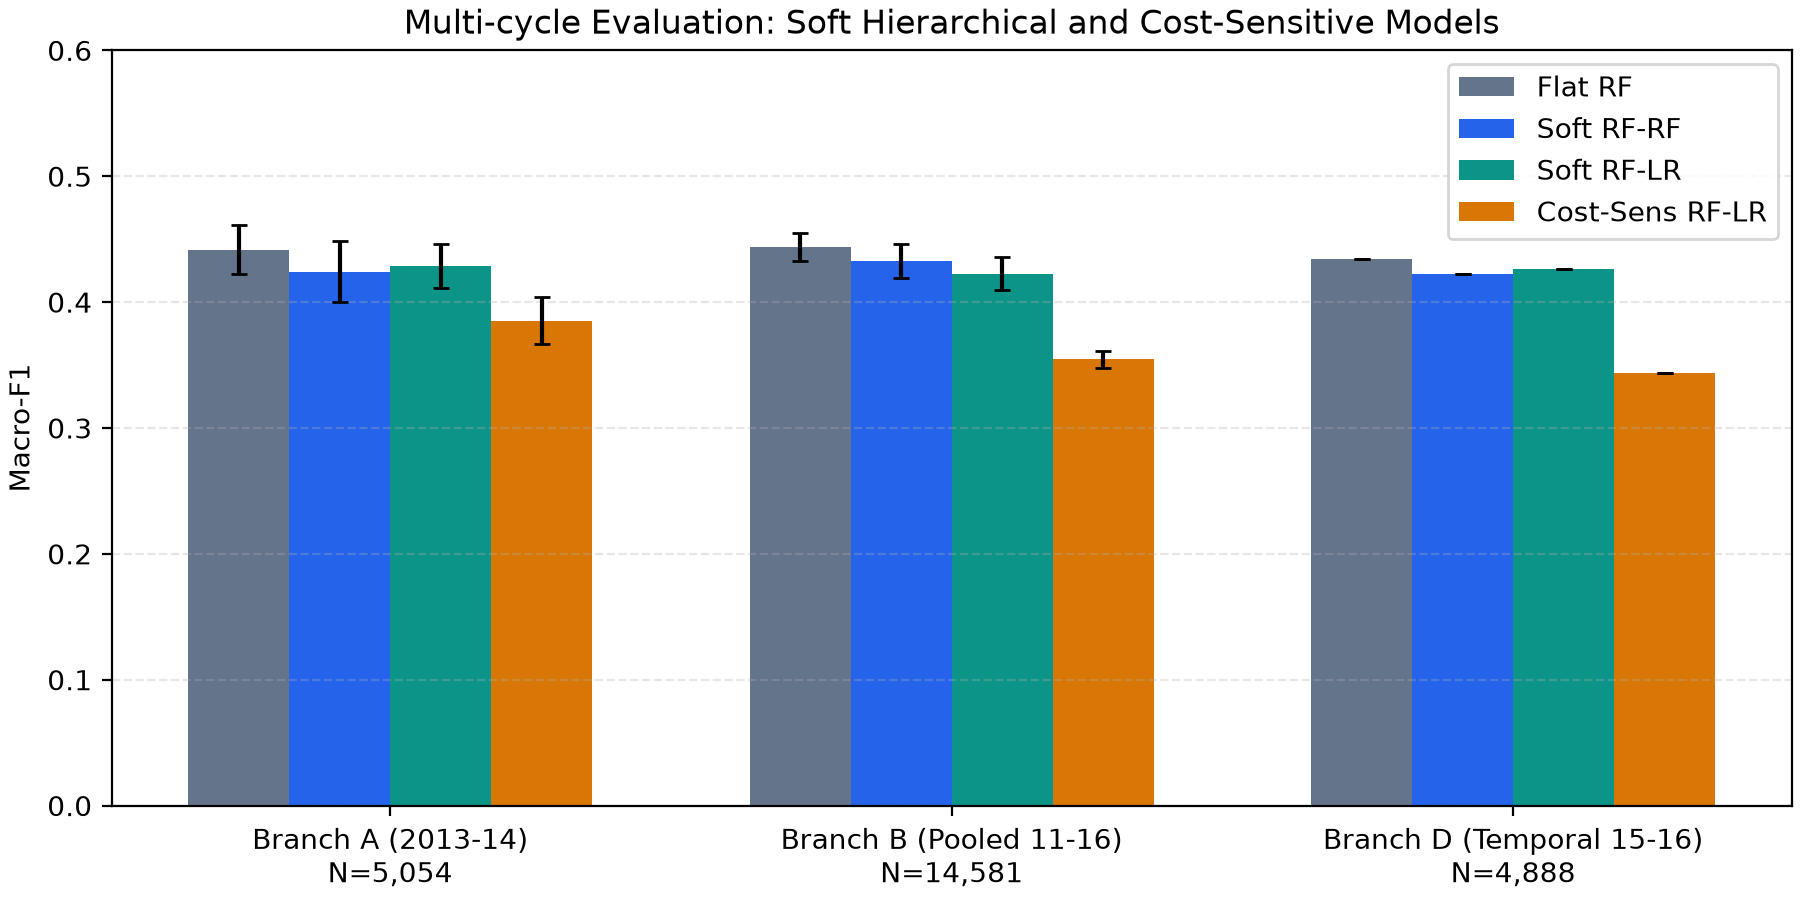
\includegraphics[width=0.85\textwidth]{figures/multicycle_soft_comparison.png}
\label{fig:multicycle-soft-temporal}
\end{figure}
\FloatBarrier

Một số phát hiện từ kiểm định dòng thời gian:
\begin{enumerate}
    \item \textbf{Độ ổn định của Balanced OLR ($E_{7a}$):} Mô hình Ordinal Logistic Regression cân bằng đạt Balanced Accuracy = \textbf{0.5073} trên tập dữ liệu tương lai (so với 0.5151 ở kiểm định chéo nội chu kỳ), mức suy giảm chỉ 1.5\%. Khả năng nhận diện ca nặng Recall $C_2^+$ đạt 59.30\%, cho thấy tính ổn định của cấu trúc siêu phẳng ranh giới song song trước hiện tượng dịch chuyển phân phối dữ liệu theo thời gian.
    \item \textbf{Đặc điểm của các mô hình phân cấp mềm và hàm phạt cao:} Các mô hình phân cấp mềm và mô hình áp dụng ma trận chi phí phạt cao ($E_{6b}$ với $M_2$) có sự sụt giảm độ chính xác tổng thể do dịch chuyển ngưỡng xác suất ngoài mẫu, cho thấy các mô hình tuyến tính có cấu trúc thứ bậc như OLR duy trì độ ổn định ngoại suy tốt hơn trên dữ liệu cộng đồng.
\end{enumerate}

\section{Thảo luận tổng hợp các phát hiện chính}
\label{sec:thao-luan-tong-hop}

Mặc dù nghiên cứu đã khảo sát 8 mô hình ($E_0 \to E_7$) nhằm đánh giá có hệ thống các hướng tiếp cận, các phát hiện thực nghiệm chính có thể được tóm lược qua \textbf{bốn mô hình tiêu biểu đại diện cho 4 tiêu chí cốt lõi} trong Bảng \ref{tab:executive-decision-matrix}.

\begin{table}{Tổng hợp các mô hình tiêu biểu theo từng tiêu chí}
\centering
\footnotesize
\setlength{\tabcolsep}{4pt}
\label{tab:executive-decision-matrix}
\begin{tabularx}{\textwidth}{p{3.2cm} p{3.0cm} p{3.2cm} X}
\toprule
\textbf{Tiêu chí xem xét} & \textbf{Mô hình tiêu biểu} & \textbf{Kết quả đạt được} & \textbf{Ý nghĩa thực tiễn và Đánh giá} \\
\midrule
\textbf{Phân loại 5 mức ($T_5$)} & \textbf{Random Forest (Tuned)} & Macro-F1 = 0.2755 \newline Weighted-F1 = 0.6437 & Mô hình cơ sở tốt nhất trên không gian phẳng gốc; phản ánh giới hạn phân tách của tập đặc trưng sinh lý ngoại vi. \\
\midrule
\textbf{Macro-F1 cao nhất trên $T_3$} & \textbf{$E_2$ (Hard RF--RF Tuned)} & Macro-F1 = \textbf{0.4586} \newline BalAcc = 0.4745 & Đạt điểm Macro-F1 cao nhất nhưng có nguy cơ bỏ sót 98 ca nặng ($C_2^+$) thành bình thường ($C_0$) do sai số một chiều ở Stage 1. \\
\midrule
\textbf{Cân bằng giữa các lớp} & \textbf{$E_{7a}$ (Balanced OLR)} & BalAcc = \textbf{0.5151} \newline Temporal BalAcc = \textbf{0.5073} & Phân bổ độ nhạy tương đối đồng đều trên cả 3 nhóm triệu chứng và duy trì độ ổn định tốt qua kiểm định ngoại suy theo thời gian. \\
\midrule
\textbf{Giảm bỏ sót ca nặng} & \textbf{$E_{6b}$ (Soft Bayes Risk, $M_1$)} & Bỏ sót $C_2^+$ còn \textbf{62 ca} \newline (giảm \textbf{48.3\%} so với $E_1$), BalAcc = 0.5025 & Thích hợp cho mục tiêu sàng lọc y tế dự phòng; giảm số ca nặng bị bỏ sót thành bình thường từ 120 ca ($E_1$) xuống 62 ca (và 19 ca với $M_2$). \\
\bottomrule
\end{tabularx}
\end{table}


Ý nghĩa và vai trò của từng mô hình tiêu biểu:
\begin{enumerate}
    \item \textbf{Random Forest Tuned (Mô hình đối chuẩn trên $T_5$):} Là mô hình học máy cơ sở phù hợp nhất trên không gian phẳng 5 lớp gốc, đạt Macro-F1 = $0.2755 \pm 0.0270$ và Weighted-F1 = $0.6437 \pm 0.0087$. Mô hình này xác lập mốc đối chuẩn và phản ánh rõ nét đặc tính phân tách của các đặc trưng sinh lý ngoại vi dạng bảng.
    \item \textbf{$E_2$ Hard RF--RF Tuned (Tối ưu Macro-F1 trên $T_3$):} Đạt Macro-F1 cao nhất trong các mô hình $T_3$ được khảo sát (\textbf{0.4586}), cải thiện so với mô hình phẳng $E_0$ (0.4354). Tuy nhiên, mô hình thể hiện đặc điểm sai số một chiều khi có 98 ca nặng ($C_2^+$) bị gán nhãn $C_0$ tại Stage 1 (so với 120 ca ở $E_1$).
    \item \textbf{$E_{7a}$ Balanced OLR (Cân bằng phân phối và ổn định theo thời gian):} Đạt Balanced Accuracy cao nhất (\textbf{0.5151 $\pm$ 0.0152}), phân bổ độ nhạy đồng đều trên cả 3 mức độ ($C_0: 61.2\%$, $C_1: 32.9\%$, $C_2^+: 60.4\%$). Đồng thời, mô hình duy trì độ ổn định tốt với Balanced Accuracy = \textbf{0.5073} trên tập kiểm định tương lai độc lập NHANES 2015--2016.
    \item \textbf{$E_{6b}$ Soft Bayes Risk (Điều chỉnh sự đánh đổi bảo vệ ca nặng):} Nhờ tích hợp ma trận chi phí bất đối xứng, mô hình $E_{6b}$ với ma trận $M_1$ đã giảm \textbf{48.33\%} số ca nặng bị bỏ sót (từ 120 ca xuống còn \textbf{62 ca}) trong khi vẫn duy trì Balanced Accuracy = \textbf{0.5025 $\pm$ 0.0163}. Khi áp dụng ma trận phạt cao $M_2$, số ca bỏ sót tiếp tục giảm xuống \textbf{19 ca} (giảm 84.17\%), đổi lại sự gia tăng có kiểm soát của các ca báo động nhầm.
\end{enumerate}

Dựa trên các mô hình tiêu biểu này, nghiên cứu trả lời năm câu hỏi khoa học ban đầu:
\begin{itemize}
    \item \textbf{RQ1 (Đóng góp đặc trưng):} Tiền sử bệnh mạn tính ($F_2$) và lối sống/nhân khẩu ($F_3, F_4$) nâng Macro-F1 từ 0.1900 lên 0.2707; trong khi các xét nghiệm máu đơn thuần ($F_1$) chỉ đóng góp hạn chế do độ đặc hiệu thấp.
    \item \textbf{RQ2 (Độ chi tiết nhãn):} Hiệu năng thay đổi rõ rệt từ $T_2$ (0.6639) sang $T_5$ (0.2630), trong đó bước chuyển lớn nhất diễn ra tại $T_2 \to T_3$ (-34.4\%) do lớp nhẹ $C_1$ có độ tương đồng phân phối sinh lý lớn với lớp tối thiểu $C_0$.
    \item \textbf{RQ3 (Mở rộng dữ liệu):} Việc mở rộng cỡ mẫu lên $14.581$ đối tượng giúp ổn định Balanced Accuracy nhưng không làm tăng đáng kể Macro-F1 trên không gian 5 mức.
    \item \textbf{RQ4 (Phân cấp cứng):} Cấu hình $E_2$ tối ưu Macro-F1 lên 0.4586 nhưng tồn tại đặc điểm lan truyền sai số một chiều với 98 ca nặng bị phân loại nhầm ở Stage 1.
    \item \textbf{RQ5 (Phân cấp mềm, Chi phí Bayes \& Thứ bậc):} Phân cấp mềm tối ưu chi phí Bayes ($E_{6b}$) giúp giảm từ 48.33\% (62 ca với $M_1$) đến 84.17\% (19 ca với $M_2$) số ca nặng bị bỏ sót; trong khi Balanced OLR ($E_{7a}$) đạt độ cân bằng và độ ổn định ngoại suy tốt nhất.
\end{itemize}

\section{Tóm tắt chương}
\label{sec:tom-tat-chuong-4}

Chương 4 đã trình bày toàn diện các kết quả thực nghiệm trên hai hướng nghiên cứu: từ khảo sát đa mức $T_5$ làm rõ đóng góp đặc trưng và đặc tính chồng lấn phân phối sinh lý, đến khảo sát có hệ thống các mô hình phân cấp và thứ bậc trên $T_3$. Các kết quả này chứng minh rằng mỗi hướng mô hình hóa mang lại một sự đánh đổi riêng giữa độ chính xác danh nghĩa, độ nhạy từng lớp và độ ổn định ngoại suy. Các kết luận tổng kết và định hướng phát triển tiếp theo sẽ được trình bày trong Chương \ref{ch:ket-luan}.
